%%% DOCUMENT TYPE %%%%%%%%%%%%%%%%%%%%%%%%%%%%%%%%%%%%%%%%%%%%%%%%%%%%%%%%%%%%%%
%Um Platz zu sparen kann man noch No Break auf false setzen in formatting.tex
\documentclass[8pt, a4paper, twocolumn, landscape]{article}

%UM PLATZ ZU SPAREN: 1. fuer grosse Matrizen $\begin{psmallmatrix}
%a & b \\
%c & d
%\end{psmallmatrix}$.
%2. nutze \vspace{-20pt} \begin{multicols}{2}  ... \end{multicols} fuer Listen

%Besseres Design: Setze NoBreak auf True in formatting.tex

%%% SETUP %%%%%%%%%%%%%%%%%%%%%%%%%%%%%%%%%%%%%%%%%%%%%%%%%%%%%%%%%%%%%%%%%%%%%%



\usepackage{graphicx}
\usepackage{mathtools}
\usepackage{amsfonts} 
\usepackage{fancybox}
\usepackage{textcomp }
\usepackage{bbold}
\usepackage{amssymb}
\usepackage{titlesec}
\usepackage[english,ngerman]{babel}
\usepackage{mathabx} 
\usepackage{multicol}

\usepackage{amsmath} 
\usepackage[usestackEOL]{stackengine}
%\usepackage{tikz-cd}

%Abstaende Listen
\usepackage{enumitem}

\setlist{nolistsep, topsep=0pt}



%\comment{

%\begin{gather}
%3x - 5y = 0 \\
%4x - 2y = 14
%\end{gather}
%}




\title{Lineare Algebra II}
\author{Frederic Jørgensen}
\date{Erstellt: 01. Februar 2020, Zuletzt ge\aee ndert: \today \\                           % deutsche Ausgabe
	 \selectlanguage{ngerman}}
\pagestyle{headings}
\setlength{\parindent}{0pt}


%\newcommand{\sectionbreak}{\clearpage} %Seite bei jedem Abschnitt wechseln
\newcommand{\comment}[1]{}

%%% PACKAGES %%%%%%%%%%%%%%%%%%%%%%%%%%%%%%%%%%%%%%%%%%%%%%%%%%%%%%%%%%%%%%%%%%%

% Encoding

\usepackage[utf8]{inputenc}
\usepackage[T1]{fontenc}

% Geometry

\usepackage{geometry} % edit margins of paper
\usepackage{setspace} % edit line spacing
\usepackage{fancyhdr} % header, footer
\usepackage{titlesec} % edit format of titles

% Visual

\usepackage[dvipsnames]{xcolor} % colors
\usepackage{tikz} % graphics
\usepackage[framemethod=tikz]{mdframed} % frames, better theorems

% Math

\usepackage{amsmath} % math tools
\usepackage{amssymb} % math symbols
\usepackage{amsthm} % thereoms
\usepackage{mathtools} % math tools

% Referencing

\usepackage{nameref}
\usepackage{hyperref}
\usepackage{cleveref}

% Useful

\usepackage[shortlabels]{enumitem} % enumerations

% Other

\usepackage{lastpage} % get number of last page

%%% MARGINS %%%%%%%%%%%%%%%%%%%%%%%%%%%%%%%%%%%%%%%%%%%%%%%%%%%%%%%%%%%%%%%%%%%%

\geometry{a4paper, left=20mm, right=20mm, top=20mm, bottom=20mm, includehead}

%%% COLORS %%%%%%%%%%%%%%%%%%%%%%%%%%%%%%%%%%%%%%%%%%%%%%%%%%%%%%%%%%%%%%%%%%%%%

%%% COLOR DEFINITIONS %%%%%%%%%%%%%%%%%%%%%%%%%%%%%%%%%%%%%%%%%%%%%%%%%%%%%%%%%%

\colorlet{color-definition}              {Blue!20}%{SpringGreen!20}
\colorlet{color-theorem}                {Brown!25}%{Apricot!13}
\colorlet{color-proposition}            {ProcessBlue!13}% {Apricot!13}
\colorlet{color-corollary}              {Salmon!12}%{Apricot!13}
\colorlet{color-lemma}                  {Brown!7}%{Apricot!13}
\colorlet{color-remark}                 {Gray!4}
\colorlet{color-example}                {Lavender!7}
% \colorlet{color-proof}                  {FILL COLOR HERE}


%%% CAPTIONS %%%%%%%%%%%%%%%%%%%%%%%%%%%%%%%%%%%%%%%%%%%%%%%%%%%%%%%%%%%%%%%%%%%

%%% CAPTION DEFINITION %%%%%%%%%%%%%%%%%%%%%%%%%%%%%%%%%%%%%%%%%%%%%%%%%%%%%%%%%

\newcommand*{\definitionname}{Definition}
\newcommand*{\theoremname}{Theorem}
\newcommand*{\propositionname}{Proposition}
\newcommand*{\corollaryname}{Corollary}
\newcommand*{\lemmaname}{Lemma}
\newcommand*{\remarkname}{Remark}
\newcommand*{\examplename}{Example}


%%% LANGUAGE %%%%%%%%%%%%%%%%%%%%%%%%%%%%%%%%%%%%%%%%%%%%%%%%%%%%%%%%%%%%%%%%%%%

% load language setup (may also include loading packages)

%%% SETUP %%%%%%%%%%%%%%%%%%%%%%%%%%%%%%%%%%%%%%%%%%%%%%%%%%%%%%%%%%%%%%%%%%%%%%

\usepackage[english]{babel}

%%% CAPTION REDEFINITION %%%%%%%%%%%%%%%%%%%%%%%%%%%%%%%%%%%%%%%%%%%%%%%%%%%%%%%



%%% HYPHENATION %%%%%%%%%%%%%%%%%%%%%%%%%%%%%%%%%%%%%%%%%%%%%%%%%%%%%%%%%%%%%%%%



%%% TITLES %%%%%%%%%%%%%%%%%%%%%%%%%%%%%%%%%%%%%%%%%%%%%%%%%%%%%%%%%%%%%%%%%%%%%

\setcounter{secnumdepth}{2}

\titleformat{\section}[block]
{\normalfont\Large\bfseries}{\thesection}{1em}{}
\titleformat{\subsection}[block]
{\normalfont\large\bfseries}{\thesubsection}{1em}{}
\titleformat{\subsubsection}[block]
{\normalfont\normalsize\bfseries}{\thesubsubsection}{1em}{}

\titlespacing*{\section}{0pt}{3.25ex plus 1ex minus .2ex}{2.0ex plus .2ex}
\titlespacing*{\subsection}{0pt}{2.75ex plus 1ex minus .2ex}{1.0ex plus .2ex}
\titlespacing*{\subsubsection}{0pt}{2.25ex plus 0.8ex minus 0.1ex}{0.0ex plus .2ex}

%%% SPACING, LENGTHS, INDENTATION %%%%%%%%%%%%%%%%%%%%%%%%%%%%%%%%%%%%%%%%%%%%%%

\setstretch{1.05} % scaling of space between lines
% \setlength{\topsep}{FILL LENGTH HERE}
% \setlength{\itemsep}{FILL LENGTH HERE}
\setlength{\parskip}{4.0pt plus 1.0pt minus 1.0pt} % space between paragraphs
\setlength{\parindent}{0pt} % indentation of paragraphs

%%% HEADER, FOOTER %%%%%%%%%%%%%%%%%%%%%%%%%%%%%%%%%%%%%%%%%%%%%%%%%%%%%%%%%%%%%

\pagestyle{fancy}
\fancyhf{} % clear everything
\lhead{}
\chead{\large \bfseries \LaTeX{} (Math) Template}
\rhead{Page \thepage /\pageref*{LastPage}}
\lfoot{}
\cfoot{}
\rfoot{}

%%% SHORTCUTS %%%%%%%%%%%%%%%%%%%%%%%%%%%%%%%%%%%%%%%%%%%%%%%%%%%%%%%%%%%%%%%%%%

%%% SINGLE SYMBOLS %%%%%%%%%%%%%%%%%%%%%%%%%%%%%%%%%%%%%%%%%%%%%%%%%%%%%%%%%%%%

% Logic

% \forall exists
% \exists exists
% \lnot exists
% \lor exists
% \land exists
\newcommand*{\limp}{\rightarrow}
\newcommand*{\limps}{\; \limp \;} % \limp with some space around
\newcommand*{\leqv}{\leftrightarrow}
\newcommand*{\leqvs}{\; \leqvs \;} % \leqv with some space around

% Meta Logic

% \implies exists
% \iff exists

% Colon Stuff

\newcommand*{\cl}{\colon}
\newcommand*{\cleq}{\coloneqq}
\newcommand*{\eqcl}{\eqqcolon}

% Sets

\newcommand*{\N}{\mathbb{N}} % natural numbers
\newcommand*{\Z}{\mathbb{Z}} % integers
\newcommand*{\Q}{\mathbb{Q}} % rational numbers
\newcommand*{\R}{\mathbb{R}} % real numbers
\newcommand*{\C}{\mathbb{C}} % complex numbers

%%% MATH OPERATORS %%%%%%%%%%%%%%%%%%%%%%%%%%%%%%%%%%%%%%%%%%%%%%%%%%%%%%%%%%%%%

% General

\DeclareMathOperator{\id}{id}
\DeclareMathOperator{\sgn}{sgn}

%%% TEMPLATES %%%%%%%%%%%%%%%%%%%%%%%%%%%%%%%%%%%%%%%%%%%%%%%%%%%%%%%%%%%%%%%%%%

% General

% write a set definition like: { #1 | #2 }
\newcommand*{\setdefinition}[2]{
  \{#1 \mid #2\}
}

% write a nice map definition
\newcommand*{\mapdefinition}[5]{
  \begin{align*}
    #1 \cl #2 &\to     #3 \\
           #4 &\mapsto #5
  \end{align*}
}


%%% FORMATTING %%%%%%%%%%%%%%%%%%%%%%%%%%%%%%%%%%%%%%%%%%%%%%%%%%%%%%%%%%%%%%%%%

%%% SYMBOLS USED BY NUMBERINGS, ENVIRONMENTS, ... %%%%%%%%%%%%%%%%%%%%%%%%%%%%%%

% \renewcommand*\qedsymbol{$\blacksquare$} % alternative QED symbol
\renewcommand{\thefootnote}{\arabic{footnote}} % normal footnotes on page
\renewcommand{\thempfootnote}{\fnsymbol{mpfootnote}} % footnotes on minipages, e.g. in mdframed environments

%%% MDFRAMED STYLES %%%%%%%%%%%%%%%%%%%%%%%%%%%%%%%%%%%%%%%%%%%%%%%%%%%%%%%%%%%%

% thick frame and bar for title

\mdfdefinestyle{style-box}{
  linewidth=1pt,
  linecolor=Gray!20,
%   roundcorner=3pt,
  innerleftmargin=0.4\baselineskip,
  innerrightmargin=0.2\baselineskip,
  innertopmargin=0.2\baselineskip,
  innerbottommargin=0.2\baselineskip,
  frametitlebackgroundcolor=Gray!20,
  frametitleaboveskip=0.2pt,
  frametitlebelowskip=0.2pt,
  theoremseparator=,
  theoremspace=\hfill,
  theoremtitlefont=\mdseries\scshape,
  nobreak=true
}

% highlighted background

\mdfdefinestyle{style-background}{
  hidealllines=true,
  backgroundcolor=Gray!5,
  innerleftmargin=0.4\baselineskip,
  innerrightmargin=0.2\baselineskip,
  innertopmargin=0.2\baselineskip,
  innerbottommargin=0.2\baselineskip,
}

% thin frame

\mdfdefinestyle{style-thinframe}{
  linewidth=0.4pt,
  linecolor=Gray!30,
  innerleftmargin=0.5\baselineskip,
  innerrightmargin=0.5\baselineskip,
  innertopmargin=0.4\baselineskip,
  innerbottommargin=0.4\baselineskip,
}

%%% ENVIRONMENTS %%%%%%%%%%%%%%%%%%%%%%%%%%%%%%%%%%%%%%%%%%%%%%%%%%%%%%%%%%%%%%%

% Definition

\mdtheorem[
  style=style-box,
  linecolor=color-definition,
  frametitlebackgroundcolor=color-definition
]{definition}{\definitionname}[section]

% Theorem

\mdtheorem[
  style=style-box,
  linecolor=color-theorem,
  frametitlebackgroundcolor=color-theorem,
  font=\itshape
]{theorem}{\theoremname}[section]

% Proposition

\mdtheorem[
  style=style-box,
  linecolor=color-proposition,
  frametitlebackgroundcolor=color-proposition,
  font=\itshape
]{proposition}[theorem]{\propositionname}

% Corollary

\mdtheorem[
  style=style-box,
  linecolor=color-corollary,
  frametitlebackgroundcolor=color-corollary,
  font=\itshape
]{corollary}[theorem]{\corollaryname}

% Lemma

\mdtheorem[
  style=style-box,
  linecolor=color-lemma,
  frametitlebackgroundcolor=color-lemma,
  font=\itshape
]{lemma}[theorem]{\lemmaname}

\theoremstyle{remark}

% Remark

\newtheorem*{remark}{\remarkname}
\surroundwithmdframed[
  style=style-background,
  backgroundcolor=color-remark
]{remark}

% Enumeration Remark

\newenvironment{enumremark}{
  \begin{remark}
    \begin{enumerate}[(a)]
      \item[]
}{
    \end{enumerate}
  \end{remark}
}

% Example

\newtheorem*{example}{\examplename}
\surroundwithmdframed[
  style=style-background,
  backgroundcolor=color-example
]{example}

% Proof

\surroundwithmdframed[
  style=style-thinframe
]{proof}

%%% TEXT FORMATTING %%%%%%%%%%%%%%%%%%%%%%%%%%%%%%%%%%%%%%%%%%%%%%%%%%%%%%%%%%%%

% definitions

\newcommand*{\df}[1]{\colorbox{color-definition}{\emph{#1}}}



%%% DOCUMENT %%%%%%%%%%%%%%%%%%%%%%%%%%%%%%%%%%%%%%%%%%%%%%%%%%%%%%%%%%%%%%%%%%%

%%Todo:
% Definition Integritaetsring


\begin{document}
%Abstaende Gleichungen
\setlength{\abovedisplayskip}{2pt}
\setlength{\belowdisplayskip}{2pt}

\maketitle
\tableofcontents
\newpage
\begin{abstract}
	%enterlater
	\centerline{\bt{Stand zum \today}}
\end{abstract}

\newpage \ \\
\newpage
\section{Grundlagen der Linearen Algebra I}
\subsection{Grundbegriffe}

\begin{definition}
Eine Menge $X$ zusammen mit einer Verknüpfung $* : X \times X \to X $ heißt \textbf{Gruppe}, wenn folgende Axiome für die Verknüpfung gelten:
\begin{enumerate}
\item Assoziativität. $ (a*b)*c = a*(b*c) $ $ \forall a,b,c \in X$
\item neutrales und inverses Element: a. $\exists e \in X,$ sodass $e*a = a $ $\forall a \in X$, \\
b. $\forall a \in X, \exists $ $ a' \in X$ , sodass $ a'*a = e$
\end{enumerate}
Eine Gruppe heißt \textbf{abelsch}, wenn weiterhin gilt: $ a*b = b*a $ $\forall a,b \in X$ 
\end{definition}

\begin{definition}
Eine Menge $R$ zusammen mit zwei Verknüpfungen 
$+ : R \times R \to R$, $(a,b) \mapsto a+b$ (Addition) und
$\cdot : R \times R \to R$, $(a,b) \mapsto a \cdot b$ (Multiplikation)
heißt \textbf{Ring}, wenn Folgendes gilt:
\begin{enumerate}
\item R bildet zusammen mit der Addition eine abelsche Gruppe
\item Die Multiplikation ist assoziativ.
\item Es gelten Distributivgesetze:
$ (a+b)\cdot c = ac + bc $ und $ c\cdot(a+b) = ca + cb$, $\forall a,b,c \in R$
\end{enumerate}
Ein Ring heißt \textbf{kommutativ}, wenn die Multiplikation kommutativ ist.
Wir nennen einen Ring \textbf{nullteilerfrei}, wenn $\forall a,r\in R$, wenn $a\cdot b = 0 \Rightarrow a=0 \lor b=0$ 
\end{definition}

\begin{definition}
Eine Menge $K$ zusammen mit zwei Verknüpfungen 
$+ : K \times K \to K$, $(a,b) \mapsto a + b$ (Addition) und
$\cdot : K \times K \to K$, $(a,b) \mapsto a \cdot b$ (Multiplikation)
 heißt \textbf{Körper}, wenn Folgendes gilt:
\begin{enumerate}
\item Die Addition bildet eine abelsche Gruppe
\item Die Multiplikation von $K\setminus \{0\} $ bildet eine abelsche Gruppe
\item Es gelten Distributivgesetze: $ (a+b)\cdot c = ac + bc $ und $ c\cdot(a+b) = ca + bc$, $\forall a,b,c \in R$
\end{enumerate}
Jeder Körper ist ein nullteilerfreier, kommutativer Ring. Ist K ein Körper, so ist $\mathrm{char}(K) = 0$ oder eine Primzahl.
\end{definition}

\begin{definition}
Sei $K$ ein Körper. Eine Menge $V$ zusammen mit einer Addition $ + : V \times V \to V $, $(v,w) \mapsto v + w$ und einer skalaren Multiplikation  $\cdot : K \times V \to V $, $(\lambda, v) \mapsto \lambda \cdot v$ 
heißt K-Vektorraum, wenn 
\begin{enumerate}
\item $V$ bildet zusammen mit der Addition eine abelsche Gruppe
\item Für die Multiplikation von Skalaren gelten folgende Regeln:
\begin{gather*}
(\lambda + \mu) \cdot v = \lambda\cdot v + \mu\cdot v, \qquad
\lambda \cdot (v+w) = \lambda \cdot v + \lambda \cdot w \\
\mu \cdot (\lambda\cdot v) = (\mu\cdot\lambda)\cdot v, \qquad
1\cdot v = v
\end{gather*}
\end{enumerate}
\end{definition}

\begin{definition}
$W \subseteq V$ heißt \textbf{Untervektorraum} von $V$, falls:
\begin{enumerate}
\item $W \neq \emptyset$
\item $v, w \in W \implies v+w \in W$ 
\item $v \in W, \lambda \in K \implies \lambda\cdot v \in W$(
\end{enumerate}
\end{definition}

\begin{definition}
Sei $V$ ein $K$-Vektorraum mit  Basis $\mathcal{B} = (v_1, ..., v_n)$.
Dann ist der eindeutige Isomorphismus $\Phi_\mathcal{B} \in \mathrm{Hom}(K^n, V)$ mit $ \Phi_B (e_j) = v_j $ das durch $\mathcal{B}$ bestimmte Koordinatensystem $(x_1, .., x_n) = \Phi^{-1}(v)$ sind die Koordinaten von $v \in V$ bzgl. $\mathcal{B}$.
\end{definition}

\begin{definition}
Eine Teilmenge X eines K-Vektorraumes V heißt \textbf{affiner Unterraum}, falls es ein $v \in V$ und einen Untervektorraum $W \subset V$ gibt, mit
$X = v + W := \{u \in V: u = v + w: w \in W\}$ 
Wir nennen auch die leere Menge einen affinen Unterraum.
Es gilt $\mathrm{dim}(X)  := \mathrm{dim}(W)$.
\end{definition}

\begin{definition} 
F"ur Untervektorr"aume $W_1, ..., W_k \subseteq V$ bedeutet die innere direkte Summe $W_1 \oplus ... \oplus W_k$, dass 
\begin{enumerate}
\item $V = W_1 + ... + W_k$
\item $w_1 + ... + w_k = 0$ mit $w_i \in W_i$ $\implies w_1 = ... = w_k = 0$. F"ur $k = 2$ ist das "aquivalent zu $W_1 \cap W_2 = \{0\}$.
\end{enumerate}
Die Definition ist "aquivalent zu:
\begin{itemize}
\item 1. ist erf"ullt und $\mathrm{dim}(V) = \mathrm{dim}(W_1) + ... + \mathrm{dim}(W_k)$.
\item Die Vereinigung der Basen der $W_i$ ist eine Basis von $V$.
\end{itemize}
\end{definition}

\begin{definition}
Sei $(V_i)_{i \in I}$ eine Familie von $K$-Vektorr"aumen. Dann heisst 
$$
\bigoplus_{ i \in I} V_i := \{(v_i)_{i\in I} \in \prod_{i \in I} V_i | v_i = 0 \text{ f"ur fast alle } i \in I \}
$$
die "aussere direkte Summe dieser Familie, wobei das Produktzeichen f"ur das direkte Produkt steht. Im endlich dimensionalen Fall gilt $\bigoplus_{ i \in I} V_i =  \prod_{i \in I} V_i  = V_1 \times ... \times V_n$. Addition und skalare Multiplikation dieses Vektorraums sind wie auch f"ur das direkte Produkt definiert.
\end{definition}



\begin{definition}
Es gibt folgende Typen von \bt{Elementarmatrizen}:
\begin{enumerate}
\item Multiplikation der $i$-ten Zeile mit $\lambda$
\item Addition des $\lambda$-fachen der $i$-ten Zeile zur $j$-ten Zeile
\item Vertauschen der $i$-ten und $j$-ten Zeile
\end{enumerate}
\end{definition}

\subsection{Wichtige Aussagen} 

\begin{theorem} 
Jedes komplexe Polynom zerf"allt "uber $\mathbb{C}$ in Linearfaktoren.
\end{theorem}

\begin{theorem}
Jeder Vektorraum besitzt eine Basis.
\end{theorem}

\begin{theorem}
Seien $W_1, W_2 \subseteq V$ Untervektorr"aume und $F: V \rightarrow W$ linear mit $V, W$ endlich dimensional. 
Es gelten folgende Dimensionsformeln:
\begin{enumerate}
\item $\mathrm{dim}(W_1 + W_2) = \mathrm{dim}(W_1) + \mathrm{dim}(W_2) - \mathrm{dim}(W_1 \cap W_2)$
\item $\mathrm{dim}(\mathrm{Im}(F)) + \mathrm{dim}(\mathrm{Ker}(F)) = \mathrm{dim}(V)$
\item Die Dimension jeder nichtleeren Faser entspricht der Dimension des Kerns, da sie ein affiner Unterraum zum Kern ist.
\end{enumerate}
\end{theorem}

\begin{theorem}
Zu jedem Untervektorraum $W \subset V$  mit $\mathrm{dim}(V) < \infty $ gibt es einen im Allgemeinen nicht eindeutigen direkten Summanden $V = W \oplus W'$.
\end{theorem}

\begin{theorem}
Jede invertierbare Matrix ist ein endliches Produkt von Elementarmatrizen.
\end{theorem}






\begin{theorem}
Sei $V$ ein $K$-Vektorraum und $U \subset V$ ein Untervektorraum. Dann kann man auf der Menge $U/V$ auf genau eine Weise eine Addition und skalare Multiplikation definieren, so dass die kanonische Abbildung 
$$ \varrho : V \to V/U, \thickspace v \mapsto v + U$$
linear wird. Diese sind gegeben durch 
$$
(v+ U) + (w+ U) = (v + w) + U, \quad  \lambda (v+ U) = \lambda v + U.
$$
Es gilt ausserdem:
\begin{enumerate}
\item $\varrho$ ist surjektiv.
\item $Ker \thinspace \varrho = U$
\item $dim \thinspace V/U = dim\thinspace V - dim \thinspace U$ , falls $dim \thinspace < \infty$
\item Der Quotientenvektorraum $V/U$ hat die folgende universelle Eigenschaft: Ist $F: V\to W$ eine lineare Abbildung mit $U \subset Ker \thinspace F$, so gibt es genau eine lineare Abbildung $\overline{F}: V/U \to W$ mit $F = \overline{F}\circ \varrho$ 
\end{enumerate}
\end{theorem}
\begin{lemma}
Seien $A, B \in M( m \times n, K)$. Dann: 1.
$\mathrm{Rang}(A + B) \leq \mathrm{Rang}(A) + \mathrm{Rang}(B)$  \\
2. $\mathrm{Rang}(AB^T) \leq \min( \mathrm{Rang}(A), \mathrm{Rang}(B))$.
\end{lemma}
\begin{lemma}
F"ur die \textbf{Spur} gelten folgende Rechenregeln:
\begin{gather*}
\mathrm{tr}(B^\dagger) = \mathrm{tr}(\overline{B}) = \overline{\mathrm{tr}({B})}, \qquad
\mathrm{tr}(AB) = \mathrm{tr}(BA) \\
\mathrm{tr}(\lambda A + \mu B) = \lambda \mathrm{tr}(A )+ \mu \mathrm{tr}(B), \qquad
\mathrm{tr}(S A S^{-1}) = \mathrm{tr}(A)
\end{gather*}



\end{lemma}
\begin{theorem}
F"ur die \textbf{Determinante} gelten folgende Rechenregeln:
\begin{enumerate}
\item Linearit"at in Zeilen und Spalten, $\mathrm{Rang}(A) < n \Leftrightarrow \det (A) = 0 $
\item Bei Zeilen-/Spaltenvertauschung "andert die Determinante ihr Vorzeichen. Bei Addition von Zeilen/ Spalten bleibt die Determinante gleich
\item $\det (A) = \det (A^T)$
\item Sei $A$ eine obere Dreiecksmatrix. Dann $\det(A) = \mathrm{tr}(A)$.
\item $\det (A^{-1}) = \det (A)^{-1}$
\item $\det(AB) = \det (A) \det(B), \qquad \det \left( \begin{array}{cc} A_1 & C \\ 0 & A_2 \end{array} \right) = \det (A_1) \det (A_2)$
\item $\det (A) = \sum_{j = 1}^n (-1)^{i + j} \cdot a_{ij} \det (A'_{ij})$.
\end{enumerate}
\end{theorem}




\section{Verallgemeinerungen der Diagonalisierung und wichtige Normalformen}

\subsection{Trigonalisierung} %vermutlich irrelevant
\begin{definition}
Sei $F : V\ \rightarrow V$ ein Endomorphismus und $W \subset V$ ein Untervektorraum. $W$ heisst $F$-invariant, wenn $F(W) \subset W$.
\end{definition}
\begin{remark}
Ist $W \subset V$ ein $F$-invarianter Unterraum, so ist $P_{F|W}$ ein Teiler von $P_F$.
\end{remark}
\begin{definition}
Eine \bt{Fahne} $(V_r)$ eines VR $V$ ist eine Kette von UVR $V_r$ mit $dim V_r = r$ und
$$\{0\} = V_0 \subset V_1 \subset ... \subset V_n = V.$$
Ist $F \in End(V)$, so heisst die Fahne $F$-invariant, wenn alle $V_r$ $F$-invariant sind.
\end{definition}

%kann man weglassen
\comment{
\begin{remark}
F\uee r $F \in End(V)$ sind folgende Bedingungen \aee quivalent:
\begin{enumerate}
\item[(i)] Es gibt eine $F$-invariante Fahne in $V$.
\item[(ii)] Es gibt eine Basis $\mathcal{B}$ von V, so dass $M_\mathcal{B}  (F)$ eine obere Dreiecksmatrix ist.
\end{enumerate}
\end{remark}
}


\begin{theorem} \textbf{(Trigonalisierungssatz)} Sei $F$ ein Endomorphismus eines $n$-dimensionalen $K$-Vektorraumes. Dann ist $F$ genau dann trigonalisierbar, wenn $P_F$ in Linearfaktoren zerf"allt.
\end{theorem}

%kann man weglassen
\comment{
\begin{corollary} Jeder Endomorphismus eines endlich-dimensionalen komplexen Vektorraumes ist trigonalisierbar.
\end{corollary}
}

%kann man vermutlich weglassen
\comment{
\begin{remark} \bt{Rechenverfahren zur Trigonalisierung eines Endomorphismus} von $A \in M(n \times n; K)$
\begin{enumerate}
\item Pr\uee fe, dass $P_A$ in Linearfaktoren zerf\aee llt, aber A nicht diagonalisierbar ist. 
\\
Bestimme einen Eigenvektor $v_1 \in Eig(A, \lambda_1 )$ und erg\aee nze diesen zu einer Basis $\mathcal{B} := (v_1, e_i, ..., e_j)$ des $K^n$. 
\\Betrachte $S^{-1}_1 := T^{\mathcal{B}_1}_{\mathcal{K}}$ und berechne $A_2 = S_1 \cdot A \cdot S_1^{-1} = $
$\left(\begin{array}{ccccc}{
\lambda_{1}} & {*} & {\cdots} & {\cdots} & {*} 
\\ {0} & {\lambda_{2}} & {*} & {\cdots} & {*} 
\\ {\vdots} & {0} & {} & {} 
\\ {\vdots} & {\vdots} & {} & {A_{2}^{\prime}} 
\\ {0} & {0} & {} & {} & {}\end{array}\right)$
\item Bestimme einen Eigenvektor $v_2^{\prime} \in Eig(A_{2}^{\prime}, \lambda_2) $ f\uee r einen Eigenwert $\lambda_2$ von $A_{2}^{\prime}$, erg\aee nze $v_1, v_2$ zu einer Basis $\mathcal{B}_2$ des $K^n$, wobei $v_2$ wie  $v_2^{\prime}$ ist, aber zus\aee tzlich eine 0 als ersten Eintrag hat. Betrachte $S^{-1}_2 := T^{\mathcal{B}_2}_{\mathcal{K}}$ und berechne $A_3 = S_2 \cdot A \cdot S_2^{-1} = $
$\left(\begin{array}{ccccc}{
\lambda_{1}} & {*} & {\cdots} & {\cdots} & {*} 
\\ {0} & {\lambda_{2}} & {*} & {\cdots} & {*} 
\\ {\vdots} & {0} & {} & {} 
\\ {\vdots} & {\vdots} & {} & {A_{3}^{\prime}} 
\\ {0} & {0} & {} & {} & {}\end{array}\right)$

\item Das macht so oft, bis $ D := A_n =S_{n-1} \cdot A \cdot S_{n-1}^{-1}$ eine obere Dreiecksmatrix ist.
\end{enumerate}
\end{remark}
}
\subsection{Potenzen eines Endomorphismus}
\begin{theorem}
\bt{Satz von Caley-Hamilton} Sei $V$ endlichdimensional und $F \in End(V)$. Dann ist $P_F(F) = 0 \in End(V)$.
\end{theorem}
\begin{definition}
Eine Teilmenge $\mathcal{I} \subset R$ eines kommutativen Ringes $R$ heisst \bt{Ideal}, wenn gilt:
\begin{enumerate}
\item[I 1] $P, Q \in \mathcal{I} \implies P - Q \in \mathcal{I}$ (Untergruppenkriterium)
\item[I 2] $P \in \mathcal{I}, Q \in R \implies Q \cdot P \in \mathcal{I}$
\end{enumerate}


\end{definition}

\begin{definition}
Das \bt{Ideal eines Endomorph.} $F$ ist $\mathcal{I}_F := \{ P(t) \in K[t] : P(F) = 0  \} \subset K[t]$.
\end{definition}

\begin{lemma}
Jeder Endormorphismus $F$ eines reellen Vektorraums $V$ mit $\mathrm{dim}(V) \geq 1$ hat einen invarianten Unterraum mit $1 \leq \mathrm{dim}(W) \leq 2$.
\end{lemma}





\begin{theorem}
Zu jedem Ideal $\mathcal{I} \subset K[t]$ mit $\mathcal{I} \neq \{0\}$ gibt es ein eindeutiges \bt{Minimalpolynom} $M$ von $\mathcal{I}$ mit: 1.
 $M$ ist normiert \\
2. F\uee r jedes $P \in \mathcal{I}$ gibt es ein $Q \in K[t]$ mit $P = Q \cdot M$.
\end{theorem}

\begin{theorem}
Sei $n = dim (V)$ und $F \in End(V)$. Dann gilt:
1. $M_F | P_F$ $\qquad$ 2.$P_F | M_F^n$.
\end{theorem}
%Anderes aus Linalg I ergaenzen?
\begin{definition}
$F \in End(V)$ heisst \bt{nilpotent}, wenn $F^k = 0$ f\uee r ein $k \geq 1$.
\end{definition}
\begin{theorem}
Ist $F \in End(V)$ und $n = dim(V)$. Dann sind folgende Aussagen \aee quivalent:
\begin{itemize}
\item[(i)] $F$ ist nilpotent.
\item[(ii)] $F^d = 0$ f\uee r ein d mit $1 \leq d \leq n$.
\item[(iii)] $P_F = \pm t^n$.
\item[(iv)] Es gibt eine Basis $\mathcal{B}$ von $V$, so dass 
\\ \centerline{
$M_{\mathcal{B}}(F)=\left(\begin{array}{ccc}
{0} & {} & {*} \\ {} & {\ddots} & {} 
\\ {0} & {} & {0}\end{array}\right)$.
}
\end{itemize}
\end{theorem}

\subsection{Die Jordansche Normalform}
\subsubsection{Die klassische Jordan'sche Normalform}
\begin{definition}
Sei $F \in End(V)$, so dass $P_F$ in Linearfaktoren zerf\aee llt. Wenn $dim(Eig(F; \lambda_i)) < \mu (P_F; \lambda_i) =: r_i$, kann man die Dimension des Eigenraums vergr\oee ssern: 
\\ \centerline{$Eig(F; \lambda_i) \subset Ker(F - \lambda_i id_v)^{r_i} = Hau(F; \lambda_i)$. }
$Hau(F; \lambda_i)$ nennt man den \bt{Hauptraum} von $F$ zum Eigenwert $\lambda_i$.
\end{definition}

\begin{theorem} \bt{(Satz \uee ber die Hauptraumzerlegung)} 
Sei $F \in End_K(V)$ mit $P_F = \pm (t- \lambda_1)^{r_1}... (t- \lambda_k)^{r_k}$. Es sei $V_i := Hau(F, \lambda_i)$ f\uee r alle paarweise verschiedenen Eigenwerte $\lambda_1, ... , \lambda_k \in K$ von $F$. Dann:
\begin{enumerate}
\item $F(V_i) \subset V_i$, $dim(V_i) = r_i$ und $V =\bigoplus\limits_{i \in I} V_i$ mit $I= \{1, ..., k\}$.
\item $F$ hat eine Zerlegung $F = F_D + F_N$ mit
\begin{enumerate}
\item $F_D$ ist diagonalisierbar, $F_N$ ist nilpotent und $F_N$ und $F_D$ kommutieren
%\item $F_N$ und $F_D$ lassen sich als Polynome von $F$ schreiben und kommutieren insbesondere mit $F$
\item Wenn man (a) verlangt, ist diese Zerlegung eindeutig
\end{enumerate}
\end{enumerate}
\end{theorem}

\comment{
\begin{corollary}
Sei $A \in M(n \times n; K)$, so dass $P_A$ in Linearfaktoren zerf\aee llt. Dann $\exists S \in GL(n)$: 
$$
S A S^{-1}=\left(\begin{array}{cccc}{} & {} & {} & {} 
\\ {\lambda_{1} E_{r_{1}}+N_{1}} & {} & {} & {0} 
\\ {} & {} & {\ddots} & {} 
\\ {0} & {} & {} & {\lambda_{1} E_{r_{1}}+N_{1}} 
\end{array}\right)
$$
wobei f\uee r $i = 1, ... k$
\\ \centerline{$
\lambda_{1} E_{r_{1}}+N_{1} = 
\left(\begin{array}{ccc}
{\lambda_{i}} & {} & {*} 
\\ {} & {\ddots} & {} 
\\ {0} & {} & {\lambda_{i}}\end{array}\right) \in M(r_i \times r_i; K)$.}
mit nilpotenten $N_i$. Insbesondere ist $\tilde{A} = D + N$, wobei $D$ eine Diagonalmatrix und $N$ nilpotent ist und $N$ und $D$ kommutieren.
%%%
\end{corollary}
}

\begin{lemma}
\bt{(Lemma von Fitting)} Zu einem $G \in End_K(V) $ betrachte
$$d := min \{ l \in \N : Ker (G^l) =Ker(G^{l + 1}) \} \text{ und } r := \mu (P_G ; 0),$$
wobei $G^0 := id_V$. Dann gilt:
\begin{enumerate}
\item $d =min \{l : Im(G^l) = Im(G^{l + 1}) \}.$
\item $Ker (G^{d + i}) = Ker (G^d) =: U, \ Im (G^{d + i}) = Im (G^d) =: W \ \forall i \in \N$.
%\item Die R\aee ume $U := Ker (G^d)$ und $W := Im (G^d)$ sind $G$-invariant.
\item $(G|U)^d = 0$ und $G|W: W \rightarrow W$ ist ein Isomorphismus.
%\item F\uee r das Minimalpolynom von $G|U$ gilt $M_{G|U} = t^d$.
\item $V = U \oplus W$, $dim(U) = r \geq d$ %, $dim(W) = n - r$.
\comment{ \\ Insbesondere gibt es eine Basis $\mathcal{B}$ von $V$, so dass
\\ \centerline{$M_\mathcal{B}(G) =
\left(\begin{array}{ll}{N} & {0} 
\\ {0} & {C}\end{array}\right) 
$
mit  $N^d = 0$ und $C \in GL (n-r; K)$.} }
\end{enumerate}
\end{lemma}
%Satz seite 256 nochmal aufschreiben

\begin{definition}
Ein \bt{Jordanblock / Jordanmatrix} ist definiert als $$J_{k}(\lambda):=\left(\begin{array}{cccc}
{\lambda} & {1} & {} & {0} 
\\ {} & {\ddots} & {\ddots} & {} 
\\ {} & {} & {\ddots} & {1} 
\\ {0} & {} & {} & {\lambda}\end{array}\right) \in \mathrm{M}(k \times k ; K).$$ Im Fall $\lambda = 0$ gilt  $J^k = 0$ und $J^{k-1} \neq 0$. \\
Wir definieren f"ur $A \in M(k \times k, K)$ folgende Notation:
$$
A^{\oplus s} = \left( \begin{array}{ccc} A & &  \\ & \ddots & \\ & & A \end{array} \right) \in M(ks \times ks, K).
$$
\end{definition}


\begin{definition}
Sei $F \in \mathrm{End}(V)$ nilpotent und $v \in V$ beliebig mit $l = \min \{k \in \mathbb{N} |F^l(v) = 0\}$. Dann nennt man
$
(v, F(v), ..., F^{l-1}(v))
$
Jordan-Strang. Dieser ist linear unabh"angig. Im n"achsten Theorem wird Existenz einer Basis aus Jordan-Str"angen gezeigt.
\end{definition}

%Ist durch Jordansche Normalform impliziert
\comment{
\begin{theorem}
Sei $G$ ein nilpotenter Endomorphismus eines K-Vektorraums $V$ und $d$ minimal, so dass $G^d = 0$. Dann gibt es eindeutig bestimmte Zahlen $s_1, ..., s_d \in \mathbb{N}$ mit 
$$d \cdot s_d +(d - 1)s_{d-1} + ... + s_l = \mathrm{dim} V$$
und eine Basis $\mathcal{B}$ von $V,$, so dass 
$$M_\mathcal{B}(G) =
\left( \begin{array}{ccc} J_d^{\oplus s_d}(0) & & \\ & \ddots & \\ & & J_1^{\oplus s_1}(0) 

\end{array} \right)
$$
\comment{
$$
\left( \begin{array}{cccccccccc}
{J_{d}} & {} & {} & {} & {} & {} & {} & {} & {} & {}
\\ {} & {\ddots} & {} & {} & {} & {} & {} & {} & {0} & {}
\\ {} & {} & {J_{d}} & {} & {} & {} & {} & {} & {} & {}
\\ {} & {} & {} & {J_{d-1}} & {} & {} & {} & {} & {} & {}
\\ {} & {} & {} & {} & {}\ddots & {} & {} & {} & {} & {}
\\ {} & {} & {} & {} & {} & {J_{d-1}} & {} & {} & {} & {}
\\ {} & {} & {} & {} & {} & {} & {\ddots} & {} & {} & {}
\\ {} & {} & {} & {} & {} & {} & {} & {J_{l}} & {} & {}
\\ {} & {0} & {} & {} & {} & {} & {} & {} & {\ddots} & {}
\\ {} & {} & {} & {} & {} & {} & {} & {} & {} & {J_{l}}
\end{array} 
\right),$$
\\wobei $J_d$ $s_d$-mal, $J_{d-1}$ $s_{d-1}$-mal, ... und $J_l$ $s_1$-mal vorkommt.
}

\end{theorem}
}


\begin{theorem}
\bt{(Allgemeine Jordansche Normalform)}
Sei $F \in End(V)$, wobei das charakteristische Polynom von $F$ in Linearfaktoren zerf\aee llt mit
$$P_F = \pm (t - \lambda_1)^{r_1} \cdot ... \cdot (t - \lambda_k)^{r_k}.$$
\begin{enumerate}
\item Dann gibt es eine Basis $\mathcal{B}$ von $V$ mit 
$$
M_\mathcal{B}(F) = \left( \begin{array}{ccc}
B(\lambda_1) & & \\ & \ddots & \\ & & B(\lambda_k)
\end{array} \right)
$$
wobei $B(\lambda_i)$ die Bl"ocke der Hauptr"aume sind:
$$
B(\lambda_i) = \left(
\begin{array}{ccc} J_1(\lambda_i)^{\oplus s_{i1}} & & \\ & \ddots & \\ & & J_{l_i}(\lambda_i)^{\oplus s_{il_i}}
\end{array}
\right),
$$
wobei $l_i = \mu (M_F, \lambda_i)$. Der gr"osste Jordanblock hat genau die Gr"osse $l_i$, woraus sich direkt das Minimalpolynom ableiten l"asst.
\item Sei $d_{jr} = \mathrm{dim}\mathrm{Ker}(F - \lambda_j id_V)^r$ f"ur $r \geq 0$ und $d_{jr} = 0$ f"ur $r \leq 0$. Dann gilt
$$
s_{jr} = 2d_{jr} - d_{j(r + 1)} - d_{j(r-1)}.
$$
%%%% Comment / old version 
\comment{
$M_\mathcal{B}(F) = 
\left(\begin{array}{ccc}
\lambda_{1} E_{r_{1}}+N_{1} & & 0 
\\ & \ddots &  
\\ 0 & & \lambda_{k} E_{r_{k}}+N_{k}
\end{array}\right).$
\\ $\lambda_i E_{r_i} + N_i = \left(\begin{array}{ccc}
B_{1, d_1} & & 0 
\\ & \ddots &  
\\ 0 & & B_{1, d_2}
\end{array}\right)$
 besteht dabei aus Jordanbl\oee cken, welche diese Form haben:
\\ \centerline{$B_{i, d} = \left(\begin{array}{cccc}\lambda_{i} & 1 & & 
\\ & \ddots & \ddots & 
\\ & & \ddots & 1 
\\ & & & \lambda_{i}\end{array}\right). \in M( r_i \times r_i, K)$}


Es gilt $1 \leq d_i \leq \mu (M_F, \lambda_i)$ f\uee r $\forall i$.  Der gr\oee sste Jordanblock hat dabei genau die Gr\oee sse $\mu (M_F, \lambda_i)$.
}
%%%%

\item Man nennt die Elemente $\lambda_i, r_i, d_{jr}$ \bt{Invarianten} des Endomorphismus $F$. Die jordansche Normalform ist insbesonderedadurch  bis auf die Reihenfolge der Jordanbl\oee cke wegen 2. eindeutig bestimmt. Zwei komplexe Matrizen sind genau dann "ahnlich, wenn sie (bis auf Permutation der Bl"ocke) die gleiche Jordanform / die gleichen \bt{Invarianten} haben.
\end{enumerate}
\end{theorem}

\begin{corollary}
$F \in End(V)$ ist genau dann diagonalisierbar, wenn $M_F$ folgende Form hat:
\\ \centerline{$M_F = (t - \lambda_1) \cdot ... \cdot (t - \lambda_k)$,}
wobei $\lambda_1, ... , \lambda_k$ die Eigenwerte von $F$ sind.
\end{corollary}


\comment{
\begin{remark}
\bt{Rechenverfahren zur Bestimmung einer Jordan-Normalform} 
\begin{enumerate}
\item Bestimme die Eigenwerte $\lambda_1, ... \lambda_k$ der Matrix $A \in M(n \times n; K)$.
\item Bestimme die Anzahl und Gr\oee sse der Jordanbl\oee cke:

Sei $U = A - \lambda_i E_n$.
Sei $q= min\{l \ | \ dim(Ker(U^l)) = dim(Ker(U^{l+1})\}$ und $s_j^{(i)} = dim(Ker(U^j))$ mit $j \leq q$.
Die Anzahl der Jordanbl\oee cke der Gr\oee sse $j$ zum Eigenwert $\lambda_i$ ist dann gegeben durch 
\\ \centerline{$s_j^{(i)} - s_{j-1}^{(i)} +s_{j+1}^{(i)}.$}
\\
\\
\\ \textit{Kommentar :} Die Anzahl der Jordanbl\oee cke zu $\lambda_i$ ist gegeben durch die geometrische Vielfachheit von $\lambda_i$.
\item Eine jordansche Normalform l\aee sst sich anhand dieser Parameter aufstellen.
\end{enumerate}
\end{remark}
}
%---------------------------------------


\begin{remark}
\bt{Rechenverfahren: Bestimmung einer Jordan-Normalform} 
\begin{enumerate}
\item Bestimme die Eigenwerte $\lambda_1, ... \lambda_k$ der Matrix $A \in M(n \times n; K)$. Sei $\lambda$ einer Eigenwerte. F"uhre den folgenden Schritt f"ur jeden Eigenwert $\lambda_i$ aus
\item  Bestimme die Anzahl und Gr\oee sse der Jordanbl\oee cke:
\begin{itemize}
\item Setze $B_i = A - \lambda_i E_n$.
\item Berechne $d_{ir} = \mathrm{dim}(\mathrm{Ker}\left(B_i)^r\right)$ und schreibe die Zahlen "ubersichtlich auf (zB Tabelle)
\item Nun gilt nun gem"ass des Theorems f"ur die Gr"ossen der Jordanbl"ocke $s_{jr} = 2 d_{jr} - d_{j(r+1)} - d_{j(r-1)}$
\end{itemize}
\item Eine jordansche Normalform l\aee sst sich jetzt wie im Theorem aufstellen.
\end{enumerate}
\end{remark}



\begin{remark}
\bt{Rechenverfahren: Basiswechselmatrix einer Jordan-Normalform}
\begin{enumerate}
\item Bestimme die Eigenwerte $\lambda_1, ... \lambda_k$ der Matrix $A \in M(n \times n; K)$. 
\item Das folgende Verfahren muss f\uee r jeden Eigenwert $\lambda_i$ durchgef\uee hrt werden
\begin{enumerate}
\item Sei $B = A - \lambda_i E_n$. Sei $q= min\{l \ | \ Ker(B^l) = Ker(B^{l+1})\}$. Wir bezeichnen von jetzt an mit $M$ die Menge der bereits gefundenen Basisvektoren.
\item Suche $v_1^{(r)}, v_2^{(r)}, ... \in \mathrm{Ker}(B^r) \backslash \mathrm{span}(\mathrm{Ker}(B^{r-1}) \cup M)$ f"ur alle $1 \leq r \leq q$. Beginne  mit $r = q$  und gehe dann in absteigender Reihenfolge vor.
\item Die so gefundenen Jordanketten $B^{r-1} v_i^{(r)}, ..., B v_i^{(r)}, v_i^{(r)}$(Reihenfolge wichtig!) zu Jordanbl"ocken der Gr"osse $r$ werden nebeneinander in die Liste der Basisvektoren geschrieben, also 
$$
\mathcal{B} = ( ... , B^{r-1} v_i^{(r)}, ..., B v_i^{(r)}, v_i^{(r)}, ...).
$$
\item F"uhre $(b)$ mit $r-1$ durch, es sei denn $r = 1$. 
\end{enumerate}
\end{enumerate}
\end{remark}

%----------------------------

\comment{

\begin{remark}
\bt{Rechenverfahren: Basiswechselmatrix einer Jordan-Normalform}
\begin{enumerate}
\item Bestimme die Eigenwerte $\lambda_1, ... \lambda_k$ der Matrix $A \in M(n \times n; K)$. Das folgende Verfahren muss f\uee r jeden Eigenwert durchgef\uee hrt werdemn
\item Sei $U = A - \lambda_i E_n$.

Bestimme $Ker(U), ..., Ker(U^q)$ wobei $q= min\{l \ | \ Ker(U^l) = Ker(U^{l+1})\}$. 
\item Bestimme die Gr\oee sse der Jordanbl\oee cke des Eigenwerts $\lambda_i$.
\item F\uee r einen Jordanblock der Gr\oee sse $j$ bestimme einen Vektor $v_j^{(i)} \in Ker(U^q) / Ker(U^{q-1})$ zum Eigenwert $\lambda_i$. Dann ist $v_{k-1}{(i)} = (A - \lambda_i E_n)(v_k) $ f\uee r all $k = 1, ..., j-1.$
\item $\mathcal{B} = (v_1^{(1)}, ..., v_j^{(1)}, ..., v_1^{(k)}, ..., v_j^{(k)})$ ist die gesuchte Basis.

\end{enumerate}
\end{remark}
}

%15052020
\subsubsection{Die Relle Jordansche Normalform}
%aus LA I
\begin{theorem}
Sei $f \in \mathbb{R}[t]$ ein reelles Polynom vom Grad $n \geq 1$. Dann hat $f$ eine Zerlegung
$$
f = a(t - \lambda_1)...(t- \lambda_k)g_1...g_m,
$$
wobei $a \in \mathbb{R}$ und $\lambda_j \in \mathbb{R}$ die reellen Nullstellen sind und die $g_j \in \mathbb{R}[t]$ normierte quadratische Polynome ohne reelle Nullstellen sind. Insbesondere ist hier $n = k + 2m$, und falls $n$ ungerade ist muss $f$ mindestens eine reelle Nullstelle haben.
\end{theorem}

%Ausfuehrugen / Vorbereitung aus Skript uebernehmen?

\begin{definition}
Betrachte ein quadratisches Polynom $g_j \in \mathbb{R}[t]$ mit komplexen Nullstellen $\mu_j = a_j + i b_j$ und $\overline{\mu_j}$. Dann definieren wir den Matrixblock $A_j$ als
$$
A_j := \left( \begin{array}{cc}
a_j & b_j \\ -b_j & a_j
\end{array} \right).
$$

Sei$A \in M( 2 \times 2, \mathbb{R})$. Dann ist die \bt{Block-Jordanmatrix} von $A$ definiert als
$$
J_r(A) := \left( \begin{array}{cccc}
A & E_2 & & \\ & \ddots & \ddots & \\ & & \ddots & E_2 \\ & & & A.
\end{array} \right) \in M( 2r \times 2r, \mathbb{R}).
$$

\end{definition}

%Notwendige Definition machen und kompatibel machen mit vorheriger Version
\begin{theorem}
Sei $F$ ein Endomorphismus des endlich und $n$-dimensionalen $\mathbb{R}$-Vektorraums $V$. Die irreduzible reelle Faktorisierung vom charakteristischen Polynom von $F$ sei
$$
P_F(t) = \pm (t- \lambda_1)^{r_1} \cdot ... \cdot (t- \lambda_k)^{r_k} \cdot g_1^{q_1} \cdot ... \cdot g_m^{q_m}.
$$ 

Seien
$V_j = \mathrm{Ker}(F- \lambda_j id_v)^{r_j}, \quad V_j' = \mathrm{Ker}(g_j(F))^{q_j}$ f"ur $j = 1, ..., k$ bzw. $j = 1, ..., m$. 
\comment{
Sei 
$$
d_{j r}= \operatorname{dim} \operatorname{Ker}\left(F-\lambda_{j} i d_{V}\right)^{r}, \quad 
d_{j r}^{\prime}=\operatorname{dim} \operatorname{Ker}\left(g_{j}(F)^{r}\right)
$$
f"ur $r = 1, 2, ...$, und setze formal $d_{jr} = d_{jr}' = 0$ f"ur $r \leq 0$. 
}
Dann gilt:
\begin{enumerate}
\item \(\operatorname{dim} V_{j}=r_{j}\) und \(\operatorname{dim} V_{j}^{\prime}=2 q_{j}\) und \(V\) zerf"allt in $F$ -invariante Untervektorräume:
$$
V=V_{1} \oplus \cdots \oplus V_{k} \oplus V_{1}^{\prime} \oplus \cdots \oplus V_{m}^{\prime}
$$
\item Es gibt eine Basis $\mathcal{B}$ von $V$, so dass:
$$
M_\mathcal{B}(F) = \left( \begin{array}{cccccc}B(\lambda_1) & & & & & \\
& \ddots & & & & \\
& & B(\lambda_k) & & & \\
& & & C(g_1) & & \\
& & & & \ddots & \\
& & & & & C(g_m) \\
\end{array}\right)
$$
mit den Bl"ocken $B(\lambda_y)$ definiert wie in der allgemeinen Jordanschen Normalform und den Bl"ocken $C(g_y)$ definiert als 
$$
C(g_y) = \left( \begin{array}{ccc}
J_1(A_1)^{\oplus s_{i1}'}  & & \\
& \ddots & \\
& & J_{l_i'}(A_1)^{\oplus s_{il_i'}'}
\end{array} \right), 
$$
wobei $l_i'$ der Exponent von $g_i$ im Minimalpolynom $M_F$ ist. Daraus l"asst sich zusammen mit dem Theorem "uber die allgemeine Jordansche Normalform aus $l_1, ..., l_k, l_1', ..., l_m'$ das Minimalpolynom bestimmen.
%Matrix korrigieren
\comment{
$$
M_\mathcal{B}(F)=
\left(\begin{array}{cccc}J_{1}\left(\lambda_{1}\right)^{\oplus s_{11}} & & & \\ 
& \ddots & \\ & J_{r_{k}}\left(\lambda_{k}\right)^{\oplus s_{k r_{k}}} & \\ 
& J_{1}\left(A_{1}\right)^{\oplus s_{11}^{\prime}} & J_{2}\left(A_{1}\right)^{\oplus s_{12}} & \\ 
& \ddots & J_{q_{1}}\left(A_{1}\right)^{\oplus s_{i q_{1}}} & J_{1}\left(A_{2}\right)^{\oplus s_{2 q_{1}}} \\ 
& & \ddots & J_{q_{m}}\left(A_{m}\right)^{\oplus s_{m, n}}
\end{array}\right)
$$
mit $A_j = \left(\begin{array}{cc}a_{j} & b_{j} \\ -b_{j} & a_{j}\end{array}\right)$, $\mu_j = a_j + i b_j$ wie vorher
}
\item Sei 
$
d_{j r}= \operatorname{dim} \operatorname{Ker}\left(F-\lambda_{j} i d_{V}\right)^{r}, \quad 
d_{j r}^{\prime}=\operatorname{dim} \operatorname{Ker}\left(g_{j}(F)^{r}\right)
$
f"ur $r = 1, 2, ...$, und setze formal $d_{jr} = d_{jr}' = 0$ f"ur $r \leq 0$. Dann gilt
$$
s_{jr}=2 d_{j r}-d_{j(r+1)}-d_{j(r-1)}, \quad 2 s_{j r}^{\prime}=2 d_{j r}^{\prime}-d_{j(r+1)}^{\prime}-d_{j(r-1)}^{\prime}
$$
für $j=1, ..., k$ bzw. $j=1, ..., m$ und alle $r$.
\comment{
\item Das Minimalpolynom ist 
$$
M_F(t) = (t - \lambda_1)^{l_1} ... (t - \lambda_k)^{l_k} g_1^{l'_1} ... g_m^{l'_m}
$$
mit $l_j$ bzw. $l_j'$ den gr"ossten Indizes mit $s_{jl_j}\neq 0$ bzw. $s_{jl_j'}' \neq 0$.
}
\end{enumerate}
\end{theorem}



\begin{remark} \bt{Rechenverfahren zur Bestimmung reeller Jordan-Normalform}
\begin{enumerate}
\item Gehe genauso vor, wie bei der allgemeinen Jordan'schen Normalform, bis darauf, dass nun f"ur die Gr"osse der $2\times 2$ Blockdiagonalmatrizen laut Theorem gilt
$$
2s_{j r}^{\prime}=2 d_{j r}^{\prime}-d_{j(r+1)}^{\prime}-d_{j(r-1)}^{\prime}
$$
\end{enumerate}
\end{remark}

\begin{remark}  \bt{Rechenverfahren zur Bestimmung der Basiswechselmatrix reeller Jordan-Normalform}
\begin{enumerate}
\item Bestimme die Basisvektoren f"ur die komplexe Jordan'sche Normalform und betrachte im Folgenden nur noch die Basisvektoren f"ur die H"auptr"aume zu komplexen Eigenwerten.
\item In der Basis gibt es f"ur jeden Jordanstrang $v_1, ..., v_m$ zum Eigenwert $\lambda \in \mathbb{C} \backslash \mathbb{R}$ einen Jordanstrang $\overline{v_1}, ..., \overline{v_m}$ zum Eigenwert $\overline{\lambda}$. Ersetze deswegen diese beiden Jordanstr"ange in der Basis durch $\mathrm{Re}(v_1), \mathrm{Im}(v_1),..., \mathrm{Re}(v_m), \mathrm{Im}(v_m)$. 
\item Tu dies f"ur alle solche Paare von Jordanstr"angen.
\end{enumerate}
\end{remark}









\begin{lemma}
Sei $A \in M(n \times n, \mathbb{R})$. Dann gilt:
\begin{enumerate}
\item $\mathrm{Rang}_\mathbb{R}(A) = \mathrm{Rang}_\mathbb{C}(A)$
\item F"ur das Minimalpolynom von $A$ gilt $M_A = M_{A_\mathbb{C}}$, wobei man bei $A_\mathbb{C}$ die reelle Matrix $A$ als komplexe Matrix auffasst.
\end{enumerate}
\end{lemma}
\begin{corollary}
\begin{enumerate}
\item Zwei reelle Matrizen sind $"ahnlich$ "uber $\mathbb{R}$ ($A = S B S^{-1}$ mit $S \in GL(n, \mathbb{R})$) genau dann, wenn ihre Invarianten (charakteristisches Polynom und Zahlen $d_{jr}, d_{jr}'$) "ubereinstimmen.
\item Alle reellen Matrizen sind "uber $\mathbb{R}$ "ahnlich genau dann, wenn sie "ahnlich "uber $\mathbb{C}$ sind.
\item  Jede relle Matrix ist "ahnlich zu ihrer Transponierten. 
\end{enumerate}
\end{corollary}

 %relle JNF aus komplexer JNF berechnen siehe Serie 12 Nr 3 
 %20052020
 %noch nicht final
 \comment{
 \begin{remark} \bt{Rechenverfahren zur Bestimmung der Basis der rellen Jordanschen Normalform}
\item F"ur die Eigenwerte geht man vor wie im Rechenverfahren zur allgemeinen Jordanschen Normalform beschrieben.
\item F"ur die quadratischen Faktoren geht man so vor: Faktorisiere die irreduziblen Faktoren $(g_j)^{q_j} = (t-\mu_j)^{q_j} (t-\overline{\mu}_j)^{q_j}= $ "uber $\mathbb{C}$ und finde eine Basis zu dem Hauptraum $\mathrm{Hau}(F, \mu_j)$ so wie in der allgemeinen Jordan'schen Normalform. Sei $v \in \mathbb{C}^n$ ein zyklischer Vektor eines Jordanblocks der Gr"osse $s$. 
 
 \end{remark}
 }


\subsubsection{Matrixexponentiale}
\begin{lemma}
Seien $A, B \in M(n \times n, K)$ mit $AB = BA$. Dann gilt
\begin{itemize}
\item $
(A+B)^m = \sum\limits_{k = 0}^m \left( \begin{array}{c}m \\ k
\end{array}\right) A^k B^{m-k} .
$
\item $
\exp (A + B) = \exp (A) \exp (B)
$
\end{itemize}
\end{lemma}

\begin{lemma}
\textbf{(Matrixexponential der Jordan'schen Normalform)}
F"ur jeden Jordanblock k"onnen wir $\exp (J) = \exp (D + N) = \exp (D) \exp (N)$ mit obiger Formel berechnen.

Matrixexponentiale von Matrizen der Form $\left( \begin{array}{cc}
a & b \\ -b & a
\end{array} \right)$ (wir nennen diesen Untervektorraum $U \subseteq M(2 \times 2, \mathbb{R})$) k"onnen wir mit dem Isomorphismus $$\Phi: \mathbb{C}_\mathbb{R} \rightarrow U , \quad z = a + ib \mapsto \left( \begin{array}{cc}
a & b \\ -b & a
\end{array} \right)$$ berechnen. Denn es gilt $\exp \left( \begin{array}{cc}
a & b \\ -b & a
\end{array} \right) = \exp(\Phi(a + ib) ) = \Phi (\exp (a + ib))$.
\end{lemma}






%Jordansche Normalform fur allgemeine Koerper und Teilbarkeitstheorie vermutlich irrelevant.
 \comment{
 %Teile von Algebra Vorlesung nicht pruefungsrelevant
 \subsubsection{Jordansche Normalform f"ur allgemeine K"orper}
 
 \begin{definition}
 Sei $f = t^n + a_{n-1}t^{n-1} + ... + a_0 \in K[t]$ ein Polynom vom Grad $n$. Dann ist die Begleitmatrix von $f$ die Matrix 
 $$
 B_{f}:=\left(\begin{array}{ccccc}-a_{n-1} & 1 & 0 & \cdots & 0 \\ -a_{n-2} & 0 & 1 & \cdots & 0 \\ \vdots & \ddots & \ddots & \ddots & \vdots \\ -a_{1} & 0 & \cdots & \cdots & 1 \\ -a_{0} & 0 & \cdots & \cdots & 0\end{array}\right)
 $$
 \end{definition}
 
 \begin{theorem}
 Das charakteristische Polynom und das Minimalpolynom von $B_f$ sind bis auf ein Vorzeichen gleich $f$, also:
 $$
 (-1)^n P_{B_f} = M_{B_f} = f.
 $$
 \end{theorem}
 
 \subsubsection{Teilbarkeitstheorie von Polynomen}
 \paragraph{Zusammenfassung Aussagen "uber Polynomringe K[t] aus LA1}
 \begin{itemize}
 \item Sei $R$ ein kommutativer Ring und $f, g \in R, f, g \neq 0$. Dann heisst $f|g$, dass ein $h \in R$ existiert mit $g = fh$
 \item Ein Ideal $\mathcal{I} \subset R$ des kommutativen Ringes ist ein Unterring mit $\mathcal{I}R \subset \mathcal{I}$. Explizit: f"ur $f, g \in \mathcal{I}$ gilt $f-g \in \mathcal{I}$ und f"ur $f \in \mathcal{I}, g \in R$ gilt $fg \in \mathcal{I}$. 
 \\
 Sind $\mathcal{I}_1, \mathcal{I}_2$ Ideale, ist $\mathcal{I}_1 \cap \mathcal{I}_2$ und $\mathcal{I}_1 + \mathcal{I}_2$ (kleinstes Ideal das beide enth"alt) wieder Ideale
 \item F"ur jeden K"orper $K$ ist der Polynomring $K[T]$ ein Hauptidealring, d.h. zu jedem Ideal $\mathcal{I} \subset R$, $\mathcal{I} \neq \{0\}$ gibt es ein eindeutiges Polynom $M)\mathcal{I} \in \mathcal{I}$, so dass $\mathcal{I} = \{ M_\mathcal{I}f| f\in K[T]\}$. $M_\mathcal{I}$ ist das normierte Polynom kleinsten Grades in $\mathcal{I}$ und heisst Minimalpolynom von $\mathcal{I}$.
 \item F"ur jeden K"orper ist $K[t]$ ein faktorieller Ring, hat also keinen Nullteiler
 \end{itemize}
 
 
 \begin{definition}
 F"ur Polynome $f, g \in K[t], f, g \neq 0$ definieren wir den gr"ossten gemeinsamen Teiler (ggT) als das normierte Polynom vom gr"ossten Grad, das $f$ und $g$ teilt. Dies ist auch das Minimalpolynom vom Ideal von $f K[t] + g K[t]$, also $ggT(f, g) = M_{ K[t] + g K[t]}.$
 Also existieren $a, b \in K[t]$, so dass $ggT(f, g) = af + bg$.
 \\
 Allgemeiner ist $ggT(f_1, ..., f_n)$ das Polynom gr"ossten Grades, das alle $f_j$ teilt. Wiederum gibt es dann $a_1, ..., a_n \in K[t]$, so dass 
 $$
 ggT(f_1, ..., f_n) = a_1 f_1 + ... + a_n f_n
 $$
 
 Ebenso definiert man $kgV(f_1, ..., f_n)$ als das normierte Polynom kleinsten Grades, dass durch alle $f_j$ teilbar ist. 
 $$
 kgV(f_1, ..., f_n) = M_{f_1K[t] \cap ... \cap f_n K[t]}.$$
 \end{definition}
 
 \begin{lemma}
 F"ur ein Polynom $f \in K[t]$ positiven Grades sind "aquivalent:
\begin{itemize}
\item Aus $f = gh$ folgt, dass eis ein $0 \neq c \in K$ existiert, so dass $f = cg$ oder $f = ch$. (Also hat $f$ keine nichttrivialen Teiler, also nur die Teiler $c \in K$ und $cf$, ist also irreduzibel.)
\item Aus $f|gh$ f"ur $g, h \in K[t], g, h \neq 0$ folgt, dass $f|g$ oder $f|h$. (Man sagt dann auch, dass $f$ ein Primelement ist).
\end{itemize}
 \end{lemma}
 
 
 
 \begin{theorem} (Primfaktorzerlegung f"ur Polynome)
 Sei $0 \neq f \in K[t]$ ein Polynom. Dann gibt es irreduzible normierte Polynome $p_1, ..., p_n \in K[t]$ positiven Grades und $c \in K$ $c\neq 0$, so dass
 $$
 f = cp_1 ... p_n.
 $$
 Diese Faktorisierung ist eindeutig bis auf die Anordnung der $p_j$.
 Man sagt auch $K[t]$ ist ein faktorieller Ring.
 \end{theorem}
 
 
 
 \begin{definition}
 Ein Ideal $\mathcal{I} \subset R$ des kommutativen Ringes $R$ heisst \bt{maximal}, falls $\mathcal{I} \neq R$ und es kein Ideal $\mathcal{J}$ gibt, so dass 
 $$
\mathcal{I} \varsubsetneqq \mathcal{J} \varsubsetneqq R.
 $$
 $\mathcal{I}$ heisst Prim, falls $\mathcal{I} \neq R$ und f"ur alle $f, g \in R$ gilt $fg \in \mathcal{I} \implies
  f \in \mathcal{I} \vee g \in \mathcal{I}$.
 \end{definition}
 
 \begin{remark}
 Im Fall $R = K[t]$ folgt direkt aus der Definition, dass $\mathcal{I}$ ein Primideal ist genau dann, wenn $M_\mathcal{I}$ prim. Ebenso ist $\mathcal{I}$ maximal, genau dann wenn $M_\mathcal{I}$ irreduzibel ist.
 \end{remark}
 
 \begin{lemma}
 Sei $\mathcal{I} \varsubsetneqq R$ ein Ideal im kommutativen Ring $R$ mit Eins. Dann gilt \begin{itemize}
 \item $\mathcal{I}$ ist maximal genau dann, wenn $R / \mathcal{I}$ mit der von $R$ geerbten Addition und Multiplikation ein K"orper ist.
 \item $\mathcal{I}$ ist prim genau dann, wenn $R/ \mathcal{I}$ nullteilerfrei ist.
 \end{itemize}
 Hierbei ist $R / \mathcal{I} = R / \sim$ mit $f \sim g \Leftrightarrow f - g \in \mathcal{I}$ definiert. Man schreibt $f + \mathcal{I} \in R / \mathcal{I}$ f"ur die "Auivalenzklasse von $f \in R$. 
 \end{lemma}
 
 
 %nicht pruefungsrelevantes Kapitel

 \begin{definition}
 Wir definieren die Matrix
 $$
 \tilde{E}_n =
\left(\begin{array}{cccc}0 & 0 & \cdots & 0 \\ \vdots & \ddots & \ddots & \vdots \\ 0 & 0 & \cdots & 0 \\ 1 & 0 & \cdots & 0\end{array}\right) \in M(n \times n, K)
 $$
 und 
 $$
 \tilde{J_r}(A)
=\left(\begin{array}{ccccc}A & \tilde{E}_{n} & & & \\ & A & \tilde{E}_{n} & & \\ & & \ddots & \ddots & \\ & & & \ddots & \tilde{E}_{n} \\ & & & & A\end{array}\right) \in M(n r \times n r, K).
 $$
 \end{definition}
 
 
 \begin{theorem}
 Sei $V$ ein endlich dimensionaler $k$-Vektorraum und $F \in End(V)$. Sei
 $$
 P_F = \pm p_1^{r_1} .... p_k^{r_k}
 $$
 die Faktorisierung in irreduzible normierte Polynome $p_1, ..., p_k$, die paarweise verschieden sind. Dann gibt es eine Basis $\mathcal{B}$ von $V$, si dass $M_\mathcal{B}(F)$ blockdiagonal ist mit Diagonalbl"ocken der Form $\tilde{J_r}(B_{p_f})$ mit $j = 1, ..., k$ und $r = 1, ..., r_j$.
 \\ Sei dabei $s_{jr}$ die Anzahl Jordanbl"ocke der Gr"osse $\tilde{J_r}(B_{p_j})$. 
 Dann gilt f"ur alle $J$
 $$
 \sum\limits_{r = 1}^{r_j} s_{jr} = r_j \mathrm{deg} p_j
 $$
 und 
 $$
 s_{jr} = \frac{1}{\mathrm{deg}  p_j}(2 \mathrm{dim} \mathrm{Ker} (p_j(F)^r) -\mathrm{dim} \mathrm{Ker}(p_j(F)^{r+1}) - \mathrm{dim} \mathrm{Ker}(p_j(F)^{r-1}).
 $$
 Insbesondere ist die Jordan'sche Normalform bis auf eine Permutation der Diagonalbl"ocke eindeutig.
  
 \end{theorem}
 
 %27052020
 \begin{theorem}
 Sei $V$ ein endlich dimensionaler $K$-Vektorraum und $F \in \mathrm{End}(V)$ mit $P_f = \pm p_1^{r_1} ... p_r^{r_k}$ als irreduzible Faktorisierung. Sei 
 $$
 V_k = \mathrm{Ker}(p_j(F)^{r_j}).
 $$
 Dann sind alle $V_k$ $F$-invariant und
 $$
 V = V_1 \oplus ... \oplus V_k.
 $$
 Das charakterische Polynom der Einschr"ankung $F|V_j$ ist
 $$
 P_{F|V_j} = \pm p_j^{r_j}.
 $$
 Insbesondere als $\mathrm{dim}_K(V_j) = r_j \mathrm{deg}(p_j)$.
 \end{theorem}


}


%Diesen Abschnitt muss man in einem anderen Abschnitt, zB bei den euklidischen und unitaeren Vektorrauemen, sinnvoll als subsection eingliedern
\subsection{Die Singul"arwertzerlegung und ihre Anwendung in Optimierungsproblemen}
\subsubsection{Die Singul"arwertzerlegung}

\begin{definition}
Man schreibt als Notation $\overline{V}^T = \tilde{V}^{\dagger}$.
\end{definition}

\begin{definition} \textbf{(Singul"arwertzerlegung)} Sei $K = \mathbb{R}$ oder $K = \mathbb{C}$ und $A \in M(m \times n, K)$. Dann gibt es orthogonale  / unit"are Matrizen $U \in O(m)$ / $U \in U(m)$, $V \in O(n)$ / $V \in U(n)$ und eine " diagonale Matrix  " $D\in M(m \times n, \mathbb{R})$ der Form 
$$
D=\left(\begin{array}{cccc}\sigma_{1} & 0 & \dots & 0 \\ 0 & \sigma_{2} & \dots & 0 \\ \vdots & & \ddots & \vdots\end{array}\right)
$$
mit nichtnegativen Diagonaleintr"agen $\sigma_j$, so dass
$$
A = U D V^\dagger.
$$
Diese Zerlegung heisst Singul"arwertzerlegung und die Diagonaleintr"age von $D$ $\sigma_1 \geq \sigma_2 \geq ... \geq \sigma_{\mathrm{min}(m,n)}$ heissen Singul"arwerte von $A$. Sie folgt aus dem Spektralsatz.

\end{definition}

\begin{remark}
Der Rang von $A$ entspricht dem Rang von $D$.
\end{remark}


\begin{corollary}
Zu $A \in M(m \times n, K)$ vom Rang $r$ gibt es gibt es orthogonale  / unit"are Matrizen $\tilde{U} \in M(m \times r, K)$, $\tilde{V} \in M(n \times r, K)$ mit orthonormalen Spalten und eine eine invertierbare Diagonalmatrix $\tilde{D} = \mathrm{diag}(\sigma_1, ..., \sigma_k) \in M(r \times r, \mathbb{R})$, so dass 
$$
A = \tilde{U} \tilde{D} \tilde{V}^\dagger.
$$
\end{corollary}

\begin{remark}
Sei $A = U D V^\dagger$ wie im obigen Theorem. Sei $r = \mathrm{Rang}(A)$. Zerlege $U = \left(U_1 | U_2\right)$, $V = \left( V_1 | V_2\right)$ mit $U_1, V_1$ jeweils den ersten $r$ Spalten. Dann ist $\mathrm{Im}(V_2) = \mathrm{Ker}(A)$ und $\mathrm{Im}(U_1) = \mathrm{Im}(A).$
\end{remark}


\begin{remark}
Um die Zerlegung aus obigem Korollar aus obigem Theorem zu erhalten, ordnet man die Singul"arwerte und definiert $\tilde{U}$ als die ersten $r$ Spalten von $U$ und $\tilde{V}$ als die ersten $r$ Spalten von $V$.

Umgekehrt erh"alt man $U$ aus $\tilde{U}$ bzw. $V$ aus $\tilde{V}$ indem man die durch die Spalten gegebene orthonormale Familie zu einer ONB erweitert und die entstehenden Vektoren als zus"atzliche Spalten schreibt. Bei $D$ f"ullt man die restlichen Zeilen mit $0$ auf.
\end{remark}



\begin{definition}
Die ersten $\mathrm{min}(m, n)$ Spalten von $U$ bzw. $V$ sind linke bzw. rechte Singul"arwerte von $A$. Man nennt Einheitsvektoren $u \in K^m$, $v \in K^n$ linke bzw. rechte Singul"arvektoren zum Singul"arwert $\sigma \in \mathbb{R}_{\geq 0}$, falls gilt
$$
Av = \sigma u \text{ oder } A^\dagger u = \sigma v
$$
\end{definition}

\begin{corollary}
Sei $F \in \mathrm{Hom}(V, W)$ mit $V, W$ endlich dimensional und unit"ar / euklidisch. Dann gibt es Orthonormalbasen $\mathcal{A}$ und $\mathcal{B}$, so dass 
$$
M^\mathcal{A}_\mathcal{B}(F) = D
$$
Diagonalform mit nichtnegativen Diagonaleintr"agen hat.
\end{corollary}


\begin{lemma}
Sei $A \in M (m \times n, K)$ eine beliebige Matrix vom Rang $r$. Dann sind die hermiteschen / symmetrischen Matrizen $\overline{A}^T A$, $A\overline{A}^T$ positiv semidefinit und haben Rang $r$. Es gilt
$$
\mathrm{Ker} \overline{A}^T A = \mathrm{Ker} A
$$
und
$$
\mathrm{Im} A \overline{A}^T = \mathrm{Im} A.
$$
\end{lemma}



\begin{remark}
Die Singul"arwerte von $A$ sind durch $A$ eindeutig bestimmt und sind die Wurzeln der gr"ossten $\mathrm{min}(m, n)$ Eigenwerte von $AA^\dagger$.. Die Matrizen $U$ und $V$ sind aber nicht ganz eindeutig bestimmt.
\end{remark}

%SVD Berechnung remark
\begin{remark} \bt{(Berechnung der Singul"arwertzerlegung)}
Sei $A \in M(m \times n, K)$.
\begin{enumerate}
\item Setze $B = A^\dagger A$ und bestimme die Eigenwerte $\lambda_1 \geq ... \geq \lambda)n \geq 0$ mit und orthogonalen Eigenvektoren $v_1, ..., v_n$ von $B$.
\item Setze $u_i = \frac{1}{\sqrt{\lambda_i}} A v_i$ f"ur $i = 1, ..., r$, wobei $\lambda_r$ der letzte positive Eigenwert ist.
\item Erg"anze $u_{r+1}, ..., u_m$ orthogonal zu $u_1, ..., u_r$.
\item Setze $U = (u_1, ..., u_m)$, $V = (v_1, ..., v_n)$, $D = \mathrm{diag}(\sqrt{\lambda_1}, ..., \sqrt{\lambda_k}, 0, ..., 0) \in M(m \times n, K)$.
\end{enumerate}
\end{remark}


%Analogon Satz Courant Fischer
\begin{corollary}
Sei $A \in M(m \times n, K)$ eine Matrix und die Singul"arwerte von $A$ gegeben durch
$$
\sigma_1 \geq ... \geq \sigma_p \geq 0.
$$
Dann folgt aus dem Satz von Courant-Fischer:
$$
\sigma_j = \min\limits_{U \subset K^n \atop \mathrm{dim}U = n-j+1} \left(   \max\limits_{u \in U \atop u \neq 0} \frac{\|Au\|}{\|u\|}\right) = \min\limits_{U \subset K^m \atop \mathrm{dim} U = m - j + 1} \left(   \max\limits_{ u \in U \atop u \neq 0 } \frac{ \|A^\dagger u\| }{ \|u\| } \right).
$$
\end{corollary}


\begin{definition}
Die Spektralnorm (2-Norm) einer Matrix $A \in M(m \times n, K($ ist der maximale Singul"arwert von $A$.
$$
\|A\|_{2}:=\sigma_{1}(A)=\max _{u \in K^n \atop u \neq 0} \frac{\|A u\|}{\|u\|}=\max _{u \in K^n \atop \|u\|=1}\|A u\|
$$
\end{definition}

\begin{remark}
Allgemeiner kann man f"ur $F \in \mathrm{Hom}(V, W)$, $V, W$ endlich dimensionale normierte Vektorr"aume, so eine Operatornorm definieren:
$$
\|F\|_{V, W} = \max\limits_{ v \in V \atop v \neq 0} \frac{\|F(v)\|_W}{\|v\|_V}.
$$
\end{remark}

%Es gab einen zusaetzlichen Abschnitt ueber die Anwendung der SVD in Regression und Pseudoinverse, der mir aber als irrelevant fuer die Klausur erschien und eher in den Bereichn Numerik faellt

%13052020

\subsubsection{Approximation von Matrizen durch Matrizen kleinen Ranges}
\begin{definition}
Sei $A = (a_{ij}) \in M( m \times n, K)$. Dann definieren wir die Frobeniusnorm von $A$ als
$$
\|A\|_F := \sqrt{\sum\limits_{i = 1}^m \sum\limits_{j = 1}^n |a_{ij}^2|} = \sqrt{\mathrm{tr}(A^\dagger A)}.
$$
Das ist die euklidische Norm von der Matrix aufgefasst als $m \cdot n$-Vektor, kommt also von folgendem Skalarprodukt auf $M(m \times n, K)$:
$
\scp{A}{B} = \mathrm{tr}(B^\dagger A).
$
\end{definition}



\begin{lemma}
Sei $A \in M( m \times n, K)$ und $U \in U(m)$, $V \in U(n)$. Dann:
$$
\| A \|_F = \|UAV\|_F.
$$
Insbesondere ist also f"ur $p = \min(m, n)$ dann
$
\|A\|_F =  \sqrt{\sigma_1^2 + ... + \sigma_p^2}.
$
\end{lemma}

\begin{theorem} \textbf{(Eckart-Young-Mirsky)} Sei $A = UDV^\dagger$ die Singul"arwerte von $A$ und seien die Singul"arwerte $\sigma_1 \geq  \sigma_2 \geq...$. Seien $u_1, ..., u_m \in K^m$ die Spalten von $U$ und $v_1, ..., v_n \in K^n$ die Spalten von $V$. Seien $U_k$ und $V_k$ die Matrizen bestehend aus den ersten $k$ Spalten von $U$ bzw. $V$. Sei $D_k$ die Matrix mit den ersten $k$ gr"ossten Singul"arwerten auf der Diagonalen. Sei 
$$
A_k = U_k D_k V_k^\dagger = \sum\limits_{j = 1}^k \sigma_j u_j v_j^\dagger.
$$
Dann gilt f"ur jede Matrix $B \in M( m \times n, K)$ vom Range $\leq k$, dass
$$
\|A - B\|_F \geq \|A - A_k \|_F = \sqrt{\sum\limits_{j = k+1}^r \sigma_j^2}.
$$
\end{theorem}

\begin{remark}
Es gilt f"ur jede Matrix $B \in M( m \times n, K)$ vom Rang $\leq k$, dass \\
$
\|A - B\|_2 \geq \|A - A_k \|_2 = \sigma_{k+1},
$
wobei $A_k$ wie oben ist.
\end{remark}

\begin{corollary}
Sei $A, B \in M(m \times n, K)$ und $i, j = 1, 2, ...$ beliebig. Dann gilt
$$
\sigma_{i+j-1} (A+B) \leq \sigma_i(A) + \sigma_j(B), 
$$
wobei $ \sigma_i(A)$ der $i$-te Singul"arwert von $A$ ist. Ist ein Index gr"osser als $\min(m, n),$ definiert man den entsprechenden Singul"arwert als $0$.
\end{corollary}

\begin{remark}
Die Singul"arwerte von $A - A_k$ sind $\sigma_{k+1}, \sigma_{k+2}, ... .$
\end{remark}

\subsubsection{Approximation durch orthogonale Matrizen}
\begin{theorem}
Sei $A \in M(n \times n, \mathbb{C})$ und $A = UDV^\dagger$ die Singul"arwertzerlegung. Dann minimiert $R_0 = UV^\dagger$ den Abstand 
$$
\|A - R\|_F
$$
unter allen unit"aren Matrizen $R \in U(n)$.
\end{theorem}

\section{Euklidische und unit\aee re Vektorr\aee ume}

\subsection{Das kanonische Skalarprodukt}
\begin{definition}
Das \bt{kanonische Skalarprodukt im $\mathbb{R}^n$} ist die Abbildung $$\langle\quad, \quad\rangle: \mathbb{R}^{n} \times \mathbb{R}^{n} \rightarrow \mathbb{R}, \quad(x, y) \mapsto\langle x, y\rangle  =  x^T \cdot y.$$
\\Mit diesen Eigenschaften (definieren allg. Skalarprodukt auf reellem VR):
\begin{enumerate}
%Bilinearitaet noch nicht komplett abgeschrieben
\item \bt{Bilinearit\aee t} $\left\langle \alpha x+ \alpha^{\prime} x^{\prime}, y\right\rangle=\alpha \langle x, y\rangle+ \alpha^{\prime}\left\langle x^{\prime}, y\right\rangle $
\\$\left\langle x, \beta y+ \beta^{\prime} y^{\prime}\right\rangle=\beta \langle x, y\rangle+ \beta^{\prime}\left\langle x, y^{\prime}\right\rangle $
\item \bt{Symmetrie} $\left\langle x, y \right\rangle = \left\langle y, x \right\rangle$
\item \bt{Positive Definitheit} $\left\langle x, x \right\rangle \geq 0$ und $\left\langle x, x \right\rangle = 0 \Leftrightarrow x = 0$.
\end{enumerate}
\end{definition}

\begin{definition}
Das \bt{kanonische Skalarprodukt im $\mathbb{C^n}$} ist die Abbildung $$\langle\quad, \quad\rangle: \mathbb{C}^{n} \times \mathbb{C}^{n} \rightarrow \mathbb{R}, \quad(x, y) \mapsto\langle x, y\rangle  = y^T \cdot \overline{x}.$$
\\Mit diesen Eigenschaften (definieren allg. Skalarprodukt auf komplexem VR):
\begin{enumerate}
\item \bt{Sesquilinearit\aee t} $\left\langle \alpha x+ \alpha^{\prime} x^{\prime}, y\right\rangle_c=\alpha \langle x, y\rangle+ \alpha^{\prime}\left\langle x^{\prime}, y\right\rangle_c $
\\$\left\langle x, \beta y+ \beta^{\prime} y^{\prime}\right\rangle_c=\overline{\beta} \langle x, y\rangle+ \overline{\beta}^{\prime}\left\langle x, y^{\prime}\right\rangle_c $
\item \bt{Symmetrie} $\left\langle w, z \right\rangle_c = \overline{\left\langle z, w \right\rangle}_c$
\item \bt{Positive Definitheit} $\left\langle z, z \right\rangle \in \mathbb{R}_+$ und $\left\langle z, z\right\rangle_c = 0 \Leftrightarrow z = 0$
\end{enumerate}
\end{definition}





\begin{definition}
Seien $x, y \in \mathbb{R}^n\backslash \{0\} $.
Der Winkel zwischen $x$ und $y$ ist definiert als
\begin{equation*}
\angle(x, y) = \arccos\left(\frac{\langle x, y\rangle}{\|x\| \cdot\|y\|}\right).
\end{equation*}
\end{definition}

\subsection{Bilinearformen und Sesquilinearformen}
\subsubsection{Bilinearformen}
%Multilinearform und Bilinearform
\begin{definition}
Seien $V_1, V_2$ Vektor\aee ume und $K$ ein K\oee rper. Eine Abbildung
\begin{equation*}
s : V_1 \times V_2 \rightarrow K
\end{equation*}
heisst \bt{bilinear} falls
\begin{enumerate}
\item[\bt{B1}] $s( \alpha v_1 + \alpha^\prime v_1^\prime, v_2) = \alpha s(v_1, v_2) + \alpha^\prime s(v_1^\prime, v_2)$ und
\item[\bt{B2}] $s(v_1, \beta v_2 + \beta^\prime v_2^\prime) = \beta s(v_1, v_2) + \beta^\prime s(v_1, v_2^\prime)$.
\end{enumerate}
\begin{enumerate}
\item[\bt{S}] Man nennt einen Bilinearform zus\aee tzlich \bt{symmetrisch}, wenn $s(v, w) = s (w, v)$
\item[\bt{A}] Man nennt sie \bt{alternierend/ schiefsymmetrisch}, falls $s(w, v) = - s(v, w)$. 
%ist bei Bilinearform egal \item[\bt{A}] Man nennt sie \bt{alternierend}, falls $s(v, v) = 0$.
\end{enumerate}
\end{definition}

\comment{
\begin{definition}
Eine \bt{Multilinearform} 
\begin{equation*}
s : V_1 \times V_2 \times ... \times V_n \rightarrow K
\end{equation*}
ist analog zur Bilinearform definiert, die Bilinearform also ein Spezialfall der Multilinearform.
\\Es gilt also f\uee r alle Koordinaten
\begin{enumerate}
\item[\bt{M1}] $s(v_1, ...,  \alpha v_k + \alpha^\prime v_k^\prime, ...,  v_n) = \alpha s(v_1, ..., v_k, ..., v_n) + \alpha^\prime s(v_1, ..., v_k^\prime, ..., v_n)$.
\end{enumerate}
\end{definition}
}



\begin{remark} Sei $V$ ein endlich dimensionaler Vektorraum, $s : V \times V \rightarrow K$ eine Bilinearform auf $V$ und $\mathcal{B} = (v_1, ..., v_n)$ eine geordnete Basis von $V$ mit dem Koordinatensystem  $\phi_\mathcal{B} : K^n \rightarrow V$.
Die darstellende Matrix von $s$ bez"uglich $\mathcal{B}$ ist $M_\mathcal{B}(s) = \left(s(v_i, v_j) \right)_{ij} \in M(n \times n, \mathbb{K})$.
Seien $v, w \in V$  mit den Koordinaten $x = \phi^{-1}_\mathcal{B}(v)$, $y = \phi^{-1}_\mathcal{B}(y)$. Dann ist
$
s(v, w)= x^T M_\mathcal{B}(s) y.
$
\comment{\left(x_{1}, \ldots, x_{n}\right)\left(\begin{array}{ccc}a_{11} & \cdots & a_{1 n} \\ \vdots & & \vdots \\ a_{n 1} & \cdots & a_{n n}\end{array}\right)\left(\begin{array}{c}y_{1} \\ \vdots \\ y_{n}\end{array}\right).}
\end{remark}

\begin{theorem}
Sei $V$ ein $n$-dimensionaler endlicher Vektorraum und $\mathcal{B}$ eine Basis von $V$. Dann ist  die Abbildung
$
s \mapsto M_{\mathcal{B}}(s)
$
von den Bilinearformen auf $M(n \times n; K)$ bijektiv und $s$ genau dann symmetrisch, wenn $M_{\mathcal{B}}(s)$ symmetrisch ist. 
\end{theorem}



\comment{
%eigentlich nicht wichtig da klar
\begin{lemma}
Seien $A, B \in M(n \times n; K)$ mit 
\begin{equation*}
x_TAy = x_TBy = 
\end{equation*}
f\uee r alle $x, y \in K^n$. Dann ist $A = B$. 
\end{lemma}
}

%11032020
\begin{theorem}\bt{(Transformationformel f"ur Bilinearformen)}
Sei $V$ eine endlichdimensionaler Vektorraum mit Basen $\mathcal{A}$ und $ \mathcal{B}$. F"ur jede Bilinearform $s$ auf $V$ gilt dann
\begin{equation*}
M_\mathcal{B}(s) =( T^\mathcal{B}_\mathcal{A})^T \cdot M_\mathcal{A}(s) \cdot T^\mathcal{B}_\mathcal{A}.
\end{equation*}
Achtung: Der Unterschied zur Transformationsformel von Endomorphismen ist $( T^\mathcal{B}_\mathcal{A})^T$ statt $( T^\mathcal{B}_\mathcal{A})^{-1}$.
\end{theorem}



\begin{definition}
Sei $s: V \times V \rightarrow K$ eine symmetrische Bilinearform. Die \bt{zu $s$ geh"orige quadratische Form} ist die Abbildung
$
q : V \rightarrow K, v \mapsto s(v, v).
$
Es gilt dann $g(\lambda v) = \lambda^2 q(v)$ f"ur  $\forall v \in V, \lambda \in K$.
Ist $V = K^n$ und $s$ durch die symmetrische Matrix $A = (a_{ij})$ gegeben, gilt:
\begin{equation*}
q(x_1, ..., x_n) = \sum\limits_{i, j = 1}^n a_{ij} x_i x_j = \sum\limits_{j = 1}^n a_{ii} x_i^2 + 2 \cdot \sum\limits_{1 \leq i < j \leq n} a_{ij}x_ix_j,
\end{equation*}
was ein homogenes quadratisches Polynom in den Unbestimmten $x_1, ..., x_n$ ist.
\end{definition}

\begin{theorem} \bt{(Polarisierung von Bilinearformen)}
Ist $\textrm{char}(K) \neq 2$, so gilt f"ur jede symmetrische Bilinearform $s$ und die zugeh"orige quadratische Form $q$:
\begin{equation*}
s(v, w) = \frac{1}{2}(q(v+w)-q(v)-q(w)) \text{ f"ur } \forall v, w \in V.
\end{equation*}
$s$ ist also aus $q$ konstruierbar.
\end{theorem}


\subsubsection{Sesquilinearformen}
\begin{definition}
Eine Abbildung $F:V \rightarrow V$ heisst \bt{semilinear}, falls 
\begin{equation*}
F(v + \lambda w) = F(v ) + \overline{\lambda} F(w) \text{ f"ur } \forall v, w \in V, \lambda \in \mathbb{C}.
\end{equation*}
Man nennt eine Abbildung $s: V \times V \rightarrow \mathcal{C}$ \bt{sesquilinear}, wenn $s$ im ersten Argument linear und im zweiten Element semilinear ist.
$s : V \times V \rightarrow \mathcal{C}$ heisst ausserdem \bt{hermitesch}, wenn gilt
\begin{enumerate}
\item[\bt{H}] $s(v, w) = \overline{s(w, v)}.$
\end{enumerate}
\end{definition}


\begin{remark}
Ist $\mathcal{A}$ eine Basis von $V$, so ist die Matrix der Sesquilinearform $s : V \times V \rightarrow \mathbb{C}$ gegeben durch $M_\mathcal{A}(s) = (s(v_i, v_j)).$
Seien $v = \phi_\mathcal{A}(x), w = \phi_\mathcal{A} (y)$ so ist 
$
s(v, w) = x^T M_\mathcal{A}(s) \overline{y}.
$
$s$ ist hermetisch genau dann, wenn 
$A^T = \overline{A}$.
\end{remark}


\begin{theorem} \bt{(Transformationsformel f"ur Sesquilinearformen)}
Sei $s : V \times V \rightarrow \mathbb{C}$ eine Sesquilinearform und $\mathcal{A}$ und  $\mathcal{B}$ Basen von $V$. Dann ist
$
M_\mathcal{B}(s) = {T^\mathcal{B}_\mathcal{A}}^T M_\mathcal{A}(s) \overline{T^\mathcal{B}_\mathcal{A}}.
$
\end{theorem}





\begin{theorem} \bt{(Polarisierung von Sesquilinearformen)}
Man hat im Komplexen für Sesquilinearformen eine \bt{Polarisierung}
$
s(v, w)=\frac{1}{4}(q(v+w)-q(v-w)+\mathrm{i} q(v+\mathrm{i} w)-\mathrm{i} q(v-\mathrm{i} w)).
$
\end{theorem}


%richtiges Zeichen ? zwischen UVR und Komplement unterscheiden.


\subsubsection{Grundbegriffe zu euklidischen  und unit"aren Vektorr"aume}
\begin{definition}
Sei $K = \mathbb{R}, \mathbb{C}$ und $V$ eine K-Vektorraum mit einer symmetrischen Bilinearform / hermiteschen Sesquilinearform $s : V \times V \rightarrow K$. 
\\ Dann heisst $s$ \bt{positiv definit}, falls $s(v, v) > 0 \ \forall v \in V/\{0\}$.
Eine solche Bilinearform / Sesquilinearform nennt man auch \bt{Skalarprodukt auf $V$}.
\\$V$ zusammen mit einem Skalarprodukt nennt man einen \bt{euklidischen Vektorraum} ($K = \mathbb{R}$) bzw. \bt{unit"aren Vektorraum} ($K = \mathbb{C}$).
\end{definition}

\begin{definition}
Die \bt{Norm} auf einem euklidischen / unit"aren Vektorraum ist eine Abbildung gegeben durch
$
 \|\cdot\|: K^{n} \rightarrow \mathbb{R}_{+}, \quad x \mapsto\|x\|:=\sqrt{\langle x, x\rangle}.
$
Sie erf"ullt folgende Eigenschaften
\vspace{-20pt}
\begin{multicols}{2}
\begin{enumerate}
\item $\|x\| \geq 0$ und $\|x\| = 0 \Leftrightarrow x= 0$
\item $ \| \alpha \cdot x \| = \mid\alpha \mid \cdot \|x \| $ 
\item $\|x+y\| \leq\|x\|+\|y\|$
\end{enumerate}
\end{multicols}
\end{definition}

\begin{remark}
Eines symmetrische (bzw. hermitesche) \bt{Matrix} $A \in M( n \times n; K)$ heisst \bt{positiv definit}, falls die zugeh"orige Bilinearform / Sesquilinearform positiv definit ist. 
\end{remark}

\begin{theorem} \bt{(Ungleichung von Cauchy-Schwarz)} Ist $V$ ein euklidischer Vektorraum, gilt f"ur alle $v, w \in V$
\begin{equation*}
|\langle v, w\rangle| \leq\|v\| \cdot\|w\|
\end{equation*}
und Gleichheit genau dann, wenn $v$ und $w$ linear abh"angig sind.
\end{theorem}

\subsubsection{Grundbegriffe zur Orthogonalit"at}
\begin{definition}
Definition. Sei \(V\) ein euklidischer bzw. unitärer Vektorraum.
\begin{enumerate}
\item Zwei Vektoren \(v, w \in V\) heißen orthogonal ($v \perp w$), wenn $\langle v, w\rangle= 0.$
\item UVR \(U, W \subset V\) orthogonal ($U \perp W$), $\Leftrightarrow
u \perp w \forall \ u \in U \text { und alle } w \in W \text {. }$
\item \textbf{Orthogonales Komplement}:
$U^{\perp}:=\{v \in V: v \perp u \ \forall \  u \in U\}$ (ist UVR).
\item Eine Familie \(\left(v_{1}, \ldots, v_{n}\right)\) in \(V\) heißt orthogonal, wenn
$v_{i} \perp v_{j} \forall i \neq j.$
Sie heißt \bt{orthonormal}, falls zusätzlich $
\|v_i\| = 1 \forall i,
$ also insgesamt $\left\langle v_{i}, v_{j}\right\rangle=\delta_{i j} \ \forall i, j.$
Eine orthonormale Basis heisst \bt{Orthonormalbasis}.
%orthogonal zeichen statt oplus
\item Ist \(V=V_{1} \oplus \ldots \oplus V_{k},\) so heißt die direkte Summe orthogonal und schreibt $V=V_{1} \obot \ldots \obot V_{k}$, falls
$V_{i} \perp V_{j} \quad \forall i \neq j.$
\end{enumerate}
\end{definition}

\begin{remark}
Sei $(v_1, ..., v_n)$ eine orthogonale Familie in $V$ mit $v_i \neq 0$ $\forall i$. Dann ist diese Familie linear unabh"angig und $(a_1 v_1, ..., a_n v_n)$ mit $a_i = \frac{1}{\|v_i\|}$ orthonormal.
\end{remark}

\begin{remark}
Sei $(v_1, ..., v_n)$ eine Orthonormalbasis von $V$ und $v \in V$ beliebig. Dann gilt:
$
v = \left\langle v, v_1 \right\rangle v_1 + ... + \left\langle v, v_n \right\rangle v_n.
$
\end{remark}

\begin{remark}
Sei $(v_1, ..., v_n)$ eine Orthonormalbasis von einem unit"aren / euklidschen Vektorraum $V$ und $v = \lambda_1 v_1 + ... + \lambda_n v_n, \ w =  \mu v_1 + ... + \mu v_n \  \in V$. Dann gilt:
$$
\left\langle v, w \right\rangle = \sum\limits_{i = 1}^n \lambda_i \overline{\mu_j} = \underbrace{\left(\begin{array}{ccc}\lambda_1 & \hdots & \lambda_n \end{array} \right)}_{\phi_\mathcal{B}^{-1}(v)} \left. \overline{\left(\begin{array}{c}\mu_1  \\ \vdots \\ \mu_n \end{array} \right)} \right\} \phi_\mathcal{B}^{-1}(w)
$$
\end{remark}

\subsection{Gram-Schmidtsches Orthogonalisierungsverfahren}
\begin{theorem} \bt{(Orthonormalisierungssatz)}
Sei $V$ ein endlichdimensionaler, euklidischer bzw. unit"arer Vektorraum und $W \subset V$ ein Untervektorraum mit der Orthonormalbasis $(w_1, ..., w_m)$. Dann gibt es eine Erg"anzung zu einer Orthonormalbasis $(w_1, ..., w_n, w_{m+1}, ..., w_n)$ von $V$. Es gilt $\mathrm{span}(w_{m+1}, ..., w_n) \perp W$.
\end{theorem}

\begin{corollary}
Jeder endlichdimensionale Vektorraum hat eine Orthonormalbasis.
\end{corollary}

\begin{corollary}
Sei $W \subset V$  Untervektorraum eines endlich dimensionalen euklidischen / unit"aren Vektorraumes $V$. Dann gilt
$
V = W \obot W^\perp \text{ und } \mathrm{dim} V = \mathrm{dim} W + \mathrm{dim} W^\perp.
$
\end{corollary}

\begin{remark}\bt{(Gram-Schmidtsches Orthogonalisierungsverfahren)}
Erg"anze $(w_1, ..., w_n)$ zu einer Basis $(w_1, ..., w_m, v_{m+1}, ..., v_n)$ von $V$. Wiederhole folgenden Schritt f"ur jedes $v_i$:

Orthonormiere $v_i$ mit $\tilde{v_i} := v_i - \left( \scp{v_i}{w_1}  w_1 +  ...  + \scp{v_i}{w_{i-1}} w_{i-1}  \right)$ und $w_i = \frac{\tilde{v_i}}{\|\tilde{v_i}\|}.$
\end{remark}

\begin{remark} \bt{(QR-Zerlegung)}
Sei $V = K^n$ und $A \in M(n \times n, K)$ invertierbar. Dann existiert eine orthogonale / unit"are Matrix  $Q$ und eine obere Dreiecksmatrix $R$, so dass $
A = Q \cdot R.$

Diese berechnet man folgendermassen. Sei $A = (a_1 | ... |a_n)$.
\begin{enumerate}
\item Konstruiere aus den $a_i$ eine ONB $(q_1, ..., q_n)$ und setze $Q = (q_1| ...|q_n)$
\item Setze $R = Q^T A$.
\end{enumerate}
\end{remark}


\begin{definition}
Sei $V$ ein unit"arer oder euklidischer Vektorraum und $W \subset V$ ein Untervektorraum mit der Orthonormalbasis $(w_1, ..., w_m)$.
Die \bt{orthogonale Projektion} auf $W$ ist dann die lineare Abbildung $P : V \rightarrow W$ gegeben durch 
$$P(v) = \scp{v}{w_1} \cdot w_1 + ... + \scp{v}{w_m}\cdot w_m.$$
\end{definition}
\subsection{Gramsche Determinante und Volumenmessung}

\begin{definition}
Seien $V$ ein euklidischer Vektorraum und $v_1, ..., v_m \in V$, wobei $m \leq n = dim V$.
Dann nennt man 
$$
G\left(v_{1}, \ldots, v_{m}\right):=\operatorname{det}\left(\begin{array}{ccc}\left\langle v_{1}, v_{1}\right\rangle & \cdots & \left\langle v_{1}, v_{m}\right\rangle \\ \vdots & & \vdots \\ \left\langle v_{m}, v_{1}\right\rangle & \cdots & \left\langle v_{m}, v_{m}\right\rangle\end{array}\right) \in \mathbb{R}
$$
die Gramsche Determinante.
\end{definition}

\begin{remark}
Es ist $G\left(v_{1}, \ldots, v_{m}\right) \geq 0$ und es gilt
$$
G\left(v_{1}, \ldots, v_{m}\right) > 0 \Leftrightarrow v_1, ..., v_m \text{ sind linear unabh"angig.}
$$
\end{remark}

\begin{definition}
Das Volumen des von  $v_1, ..., v_m$ aufgespannten Spates ist definiert als 
$$
Vol(v_1, ..., v_m) := \sqrt{G\left(v_{1}, \ldots, v_{m}\right)}.
$$
\end{definition}

\begin{theorem}\bt{(Ungleichung von Hadamard)}
Seien $v_1, ..., v_m \in V$ und $V$ ein euklidischer Vektorraum, wobei $m \leq dim V$. Dann gilt
$
Vol(v_1, ..., v_m) \leq \|v_1\| \cdot ... \cdot \|v_m\|.
$
Es besteht Gleichheit genau dann, wenn $v_i \perp v_j$ f"ur $\forall i \neq j$.


\end{theorem}

%18032020
\subsection{Orthogonale und unit"are Endomorphismen}
\begin{definition}
Sei V ein euklidischer / unit"arer Vektorraum und $F \in End(V)$. Dann heisst $F$ orthogonal / unit"ar. falls
$
\left\langle F(v), F(w) \right\rangle = \left\langle v, w \right\rangle
$ f"ur alle $v, w \in V$. Man nennt orthogonale / unit"are Abbildungen auch \bt{Isometrien}.
\end{definition}

\begin{remark}
Ein orthogonaler / unit"arer Endomorphismus erf"ullt folgende Bedingungen:
\vspace{-20pt}
\begin{multicols}{2}
\begin{enumerate}
\item $\| F(v) \| = \|v\| \forall v \in W$
\item $ v \perp w \implies F(v) \perp F(w)$
\item $F$ ist ein Isomorphismus und $F^{-1}$ orthogonal bzw. unit"ar
\item $\lambda \in K$ EW von $F \implies \ \|\lambda \| = 1$
\item $F$ erh"alt Winkel
\item Komposition orthog. / unit. Endomorphismus ist orthog. / unit.
\end{enumerate}
\end{multicols}
\end{remark}

\begin{lemma}
Gilt f"ur $F \in End(V)$ dass $\|F(v)\| = \|v\|$ f"ur alle $v \in V$, so ist $F$ orthogonal bzw. unit"ar.
\end{lemma}

\begin{definition}
Eine Matrix $A \in GL(n, \mathbb{R})$ heisst \bt{orthogonal}, falls
$
A^{-1} = A^T.
$

Eine Matrix $A \in GL(n, \mathbb{C})$ heisst \bt{unit"ar}, falls
$
A^{-1} = \overline{A}^T.
$

Eine orthogonale / unit"are Matrix $A$ heisst \bt{eigentlich orthogonal / unit"ar}, wenn $\mathrm{det}(A) = 1$.
\end{definition}

\begin{remark}
F"ur eine orthogonale bzw. unit"are Matrix $A$ gilt $|\mathrm{det}(A)| = 1$.
\end{remark}

\begin{definition}
Es sind folgende Untergruppen von $GL(n)$ definiert:
\begin{enumerate}
\item Die orthogonale Gruppe $O(n) = \{ A \in GL(n, \mathbb{R}) | A^{-1} = A^T \}$
\item Die spezielle orthogonale Gruppe $SO(n):=\{A \in O(n): \mathrm{det} A=1\}$
\item Die unit"are Gruppe U(n):=$\{A \in GL(n ; \mathbb{C}): A^{-1}= \overline{A}^T\}$
\item Die spezielle unit"are Gruppe $SU(n):=\{A \in U(n): \mathrm{det} A=1\}$.
\end{enumerate}

\end{definition}

\begin{remark}
Für \(A \in \mathrm{M}(n \times n ; K)\) sind folgende Bedingungen gleichwertig:
\begin{enumerate}
\item \(A\) ist orthogonal bzw. unitär.
\item Die Spalten von \(A\) sind eine Orthonormalbasis von \(K^{n}\).
\item Die Zeilen von \(A\) sind eine Orthonormalbasis von \(K^{n}\).
\end{enumerate}
\end{remark}


\begin{theorem}
Satz. Sei \(V\) ein euklidischer bzw. unitärer Vektorraum mit einer Orthonormalbasis \(\mathcal{B}\) und \(F \in \mathrm{End}(V)\). Dann gilt:

$F$ orthogonal bzw. unit"ar $\Leftrightarrow M_{\mathcal{B}}(F)$ orthogonal bzw. unitär.
\end{theorem}

\begin{lemma}
Ist \(A \in O(2),\) so gibt es ein \(\alpha \in[0,2 \pi[,\) so dass
E$A=\left(\begin{array}{cc}\cos \alpha  & -\sin \alpha 
\\ \sin \alpha & \cos \alpha\end{array}\right)$ 
\text{ oder  }
$$A=\left(\begin{array}{cc}\cos \alpha & \sin \alpha \\ \sin \alpha & -\cos \alpha\end{array}\right).$$
\end{lemma}

%20032020
%Der Spektralsatz sagt genau das aus
\comment{
\begin{theorem}
Jeder unitäre Endomorphismus \(F\) eines endlich dimensionalen unitären Vektorraumes besitzt eine Orthonormalbasis aus Eigenvektoren von \(F .\) 
\end{theorem}

\begin{corollary}
Zu \(A \in U(n)\) gibt es ein \(S \in U(n)\) mit
$$
 S^\dagger \cdot A \cdot S = \left(\begin{array}{ccc}\lambda_{1} & & 0 \\ & \ddots & \\ 0 & & \lambda_{n}\end{array}\right)
 $$
wobei $\lambda_{i} \in \mathbb{C}$ mit $|\lambda_{i}|=1$ f"ur $i=1, ..., n $.
\end{corollary}
}

\begin{theorem}
Sei $F$ ein orthogonaler Endomorphismus des endlichdimensionalen euklidischen Vektorraums $V$. Dann gibt es eine Orthonormalbasis $\mathcal{B}$ von $V$, so dass:
\vspace{-20pt}
\begin{multicols}{2}
\begin{itemize}
\item[] $M_\mathcal{B}(F) =$
%\left( \begin{array}{ccccccccc}
$
\begin{psmallmatrix}
{+1} & {} & {} & {} & {} & {} & {} & {} & {} 
\\ {} & {\ddots} & {} & {} & {} & {} & {} & {0} & {} 
\\ {} & {} & {+1} & {} & {} & {} & {} & {} & {} 
\\ {} & {} & {} & {-1} & {} & {} & {} & {} & {} 
\\ {} & {} & {} & {} & {}\ddots & {} & {} & {} & {} 
\\ {} & {} & {} & {} & {} & {-1} & {} & {} & {} 
\\ {} & {} & {} & {} & {} & {} & {A_1} & {} & {} 
\\ {} & {0} & {} & {} & {} & {} & {} & {\ddots} & {} 
\\ {} & {} & {} & {} & {} & {} & {} & {} & {A_k} 
\end{psmallmatrix}\\
$
%\end{array} 
%\right),$
\item[] $A_{j}=\left(\begin{array}{cc}\cos \vartheta_{j} & -\sin \vartheta_{j} \\ \sin \vartheta_{j} & \cos \vartheta_{j}\end{array}\right) \in SO(2)$ 
\item[] \ \\
\item[] mit $\vartheta_j \in (0, 2\pi), \ \vartheta_j \neq \pi$.
\end{itemize}
\end{multicols}
\end{theorem}

%Haben wir oben schon ohne die Vorraussetzung der Orthogonalit"at / Unitarit"at gezeigt.
\comment{
\begin{lemma}
Zu einem orthogonalen Endomorphismus \(F\) eines endlichdimensionalen euklidischen Vektorraumes \(V\) mit $dim (V) \geq 1\) gibt es immer einen Untervektorraum \(W \subset V\) mit
$
F(W) \subset W \text { und } 1 \leq dim (W) \leq 2 .
$
\end{lemma}
}



\subsection{Selbstadjungierte Endomorphismen}

\comment{
%Kommt Spaeter
\begin{definition}
Der zu einem Endomorphismus $F$ eines euklidischen / unit"aren Vektorraumes $V$ \bt{adjungierte Endomorphismus} $F^{ad} \in End(V)$ ist definiert durch:
$$
\scp{F(v)}{w} = \scp{v}{F^{ad}(w)}
$$
f"ur alle $v, w \in V$.
\end{definition}


%Zu adjungierten Endomorphismen
\begin{remark}
Sei $\mathcal{B}$ eine Orthonormalbasis von $V$, $F$ ein Endomorphismus und $A = M_\mathcal{B}(F)$. Dann ist der adjungierte Endormorphismus von $F$ eindeutig gegeben durch $M_\mathcal{B}(F^{ad}) = A^\dagger$.
\end{remark}
}

\begin{definition}
Ein Endomorphismus $F$ eines euklidischen / unit"aren Vektorraumes $V$ heisst \bt{selbstadjungiert}, wenn $\scp{F(v)}{w} = \scp{v}{F(w)}$ f"ur alle $v, w \in V$.
\end{definition}

\begin{theorem}
Sei $F$ ein Endomorphismus von \(V\) und \(\mathcal{B}\) eine Orthonormalbasis. Dann gilt: 

\(F\) selbstadjungiert $\Leftrightarrow M_{\mathcal{B}}(F)$ symmetrisch bzw. hermitesch.
\end{theorem}

\begin{lemma}
Die Eigenwerte eines selbstadjungierten Endomorphismus $F \in End(V)$ sind (auch im komplexen Fall) reell. 
\end{lemma}


%Der Spektralsatz sagt das auch aus (Verallgemeinerung)
\comment{
\begin{theorem}
Ist \(F\) ein selbstadjungierter Endomorphismus eines euklidischen bzw. unitären endlichdimensionalen Vektorraumes, so gibt es eine Orthonormalbasis von \(V\), die aus Eigenvektoren von \(F\) besteht. Insbesondere ist $F$ also diagonalisierbar.
\end{theorem}


\begin{theorem}
Ist \(A \in \mathbb{M}(n \times n ; K)\) eine symmetrische bzw. hermitesche Matrix, so
gibt es eine orthogonale bzw. unitäre Matrix $S$, so dass
$$
S^\dagger A S = 
\left(\begin{array}{ccc}\lambda_{1} & & 0 
\\ & \ddots & 
\\ 0 & & \lambda_{n}\end{array}\right)
$$
mit $\lambda_1, ..., \lambda_n \in \mathbb{R}$.
\end{theorem}
}

\begin{corollary}
Sind \(\lambda_{1}, ..., \lambda_{k}\) die verschiedenen Eigenwerte eines selbstadjungierten oder unitären Endomorphismus \(F\) von \(V\), so ist
$$
V= Eig (F ; \lambda_{1}) \obot ... \obot Eig(F ; \lambda_{k}).
$$
\end{corollary}

\begin{remark} \textit{(Praktische Berechnung einer Orthonormalbasis eines selbstadjungierten Endomorphismus)}
\begin{enumerate}
\item Zerlege $P_F(t) = \pm (t- \lambda_1)^{r_1} ... (t- \lambda_k)^{r_k} $ in Linearfaktoren
\item Bestimme Basen der Eigenr"aume
\item Orthonormalisiere die gefundenen Basen mit dem Gram-Schmidt-Verfahren unabh"angig voneinander in den verschiedenen Eigenr"aumen
\end{enumerate}

\end{remark}

%25032020
\begin{theorem}\bt{(Satz von Courant-Fischer)} Sei $V$ ein endlichdimensionaler euklidischer oder unit"arer Vektorraum und $F \in End(V)$ selbstadjungiert. Seien die Eigenwerte von $F$ 
$$
\lambda_1 \leq ... \leq \lambda_n.
$$
Dann gilt:
\begin{enumerate}
\item $\lambda_k = \min\limits_{U\subset V \atop \mathrm{dim} U = k} \left(   \max\limits_{x\in U \atop \ x \neq 0} \frac{\scp{x}{Fx}}{\scp{x}{x}}\right)$
\item $\lambda_k = \min\limits_{U\subset V \atop \mathrm{dim} U = n - k + 1} \left(   \max\limits_{x\in U \atop \ x \neq 0} \frac{\scp{x}{Fx}}{\scp{x}{x}}\right)$
\end{enumerate}
Die erste Minimierung ist dabei "uber die Untervektorr"aume der angegebenen Dimension.
\end{theorem}
 
\subsection{Hauptachsentransformation und Kriterien f"ur positive Definitheit}

\subsubsection{Symmetrische Bilinearformen und hermitesche Sesquilinearformen}


\begin{remark}


\textbf{Mathematikerkonvention (f"ur uns relevant)} $s(x, y) = x^T A \overline{y}$

\textbf{Physikerkonvention} $s(x, y) = \overline{x}^T A y$

\end{remark}

\comment{
R
\begin{theorem} \bt{(Hauptachsentransformation 1)} Sei $A \in M(n \times n; \mathbb{R})$ symmetrisch und $s$ die zugeh"orige Bilinearform, also $s(u, v) = u^T A v$.
\\Dann gilt:
\begin{enumerate}
\item Ist $\mathcal{B} = (w_1, ... w_n)$ eine Orthonormalbasis des $\mathbb{R}^n$, so ist
$$
M_\mathcal{B}(s) = \left(\begin{array}{ccc}\lambda_{1} & & 0 
\\ & \ddots & 
\\ 0 & & \lambda_{n}\end{array}\right), \quad \text{ also } s(w_i, w_j) = \lambda_i \delta_{ij}
$$
wobei $\lambda_1, ..., \lambda_n$ die Eigenwerte von $A$ sind (Achtung: Dies sind Eigenwerte des Endomorphismus $A$, denn Bilinearformen haben keine Eigenwerte).
\item Es gibt eine Basis $\mathcal{A}$ des $\mathbb{R}^n$, so dass
$$
M_\mathcal{A}(s) =  \left(\begin{array}{ccc}E_k & & 0 
\\ & -E_l & 
\\ 0 & & 0\end{array}\right),
$$
wobei $k$ und $l$ Invarianten der Bilinearform sind (Tr"agheitssatz von Sylvester).
\end{enumerate}
\end{theorem}

C
\begin{theorem} \bt{(Hauptachsentransformation 2)}
Sei $A \in M (n \times n, \mathbb{C} )$ hermitesch. Sei $s$ die entsprechende hermitesche Sesquilinearform auf $\mathbb{C}^n$. Dann gilt:
\begin{enumerate}
\item Es gibt eine Orthonormalbasis $\mathcal{B} = (w_1, ..., w_n)$ des $\mathbb{C}^n$, so dass 
$$
M_\mathcal{B}(s) = \left(\begin{array}{ccc}\lambda_{1} & & 0  
\\ & \ddots & 
\\ 0 & & \lambda_{n}\end{array}\right) =:D, \quad \text{ also } s(w_i, w_j) = \lambda_i \delta_{ij}
$$
wobei $\lambda_1, ..., \lambda_n$ die Eigenwerte von $A$ sind (Achtung: Dies sind Eigenwerte des Endomorphismus $A$, denn f"ur Bilinearformen / Sesquilinearformen ist der Begriff Eigenwerte sinnlos).
Alternativ: Es gibt ein $S \in O(n)$ / $S \in U(n)$ mit $S^T A \overline{S} = D$
\item Es gibt eine Basis $\mathcal{A}$ des  $\mathbb{R}^n$ / $\mathbb{C}^n$, so dass
$$
M_\mathcal{A}(s) =  \left(\begin{array}{ccc}E_k & & 0 
\\ & -E_l & 
\\ 0 & & 0\end{array}\right). =: D' 
$$
Alternativ: Es gibt ein $S \in GL(n, \mathbb{R})$ / $S \in GL(n, \mathbb{C})$ mit $S^T A \overline{S} = D'$.
\item Die Zahlen $k, l$ aus $2.$ sind gerade die Anzahl der positiven und negativen Eigenwerte von $A$ und Invarianten der Bilinearform / Sesquilinearform (Tr"agheitssatz von Sylvester).
\end{enumerate}
\end{theorem}

}


%gebuendelt
\begin{theorem} \bt{(Hauptachsentransformation)}
Sei  $A \in M (n \times n, \mathbb{R} )$ symmetrisch / $A \in M (n \times n, \mathbb{C} )$ hermitesch und  $s$ die entsprechende symmetrische Bilinearform/ hermitesche Sesquilinearform auf $\mathbb{R}^n$ / $ \mathbb{C}^n$, also $s(u, v) = u^T A v$ / $s(u, v) = u^T A \overline{v}$ Dann gilt:
\begin{enumerate}
\item Es gibt eine Orthonormalbasis des $\mathbb{R}^n$ / $\mathbb{C}^n$, so dass 
$$
M_\mathcal{B}(s) = \left(\begin{array}{ccc}\lambda_{1} & & 0 
\\ & \ddots & 
\\ 0 & & \lambda_{n}\end{array}\right) =:D, \quad \text{ also } s(w_i, w_j) = \lambda_i \delta_{ij}
$$
wobei $\lambda_1, ..., \lambda_n$ die Eigenwerte von $A$ sind (Achtung: Dies sind Eigenwerte des Endomorphismus $A$, denn f"ur Bilinearformen / Sesquilinearformen ist der Begriff Eigenwerte sinnlos).
Alternativ: Es gibt ein $S \in O(n)$ / $S \in U(n)$ mit $S^T A \overline{S} = D$.
\item Es gibt eine Basis $\mathcal{A}$ des  $\mathbb{R}^n$ / $\mathbb{C}^n$, so dass
$$
M_\mathcal{A}(s) =  \left(\begin{array}{ccc}E_k & & 0 
\\ & -E_l & 
\\ 0 & & 0\end{array}\right) =: D' 
$$
Alternativ: Es gibt ein $S \in GL(n, \mathbb{R})$ / $S \in GL(n, \mathbb{C})$ mit $S^{-1} A S = D'$.
\item Die Zahlen $k, l$ aus $2.$ sind gerade die Anzahl der positiven und negativen Eigenwerte von $A$ und Invarianten der Bilinearform / Sesquilinearform (Tr"agheitssatz von Sylvester).
\end{enumerate}
\end{theorem}

\begin{remark} \bt{(Rechenverfahren zur Bestimmung solcher $S$ und $D$)}
\begin{enumerate}
\item Schreibe $A | E_n$
\item F"uhre an $A$ simultane Zeilen- und Spaltenumformungen ($A$ ist ja symmetrisch) und an $E_n$ nur die entsprechenden Spaltenumformungen durch, bis $A$ Diagonalform hat. Dann ist $D = C_1^T \cdot ... \cdot C_k^T A \cdot C_k \cdot ... \cdot C_1$ und $S = C_k \cdot ... \cdot C_1$.
\\ Dieses Verfahren ist auch effektiv bei der "Uberpr"ufung positiver Definitheit.
\\
\\
Um im Komplexen ein $S \in GL(n, \mathbb{C})$ mit $S^T A \overline{S} = D$ zu finden, suche $T = \overline{S}$ mit $\overline{T}^T A T = D$ und konjugiere bei jeder Zeilenumformung die Koeffizienten.
\end{enumerate}
\end{remark}


\comment{
\begin{corollary}
Eine symmetrische Matrix $A \in M(n \times n; \mathbb{R})$ ist genau dann positiv definit, wenn ihre Eigenwerte positiv ist.
\end{corollary}


Fall R
\begin{theorem}
Sei $A \in M (n \times n, \mathbb{R})$ symmetrisch. Dann sind "aquivalent:
\begin{enumerate}
\item $A$ ist positiv definit, also $x^T A x > 0  \quad \forall 0 \neq x \in \mathbb{R}^n$
\item Alle Eigenwerte von $A$ sind positiv.
\item Es gibt eine Matrix $S \in GL(n, \mathbb{R})$, so dass $S^T A S$ diagonal ist mit positiven Diagonaleintr"agen 
\item Es gibt ein $T \in GL(n, \mathbb{R})$ mit $A = T^T T$.
\item Sei das charakteristischen Polynom $P_A(t) = (-1)^n t^n + \alpha_{n-1}t^{n-1} + ... + \alpha_0 \in \mathbb{R}[t].$ Dann gilt $(-1)^j \alpha_j > 0$ f"ur $j = 0, ..., n-1$. 
\item  Sei $A_k$ der $k\times k$ Block von $A$ oben links (Hauptminor). Dann $det(A_k) > 0 \ \forall k = \{1, ..., n\}$.
\end{enumerate}
\end{theorem}

Fall C
\begin{theorem}
Sei $A \in M (n \times n, \mathbb{C})$ eine hermitesche Matrix. Dann sind "aquivalent:
\begin{enumerate}
\item A ist positiv definit, also $x^TA\overline{x} > 0$ f"ur alle $x \in \mathbb{C}^n, \ x \neq 0$.
\item Alle Eigenwerte von $A$ sind positiv.
\item Es gibt ein $S \in GL(n, \mathbb{C})$, so dass $S^TA\overline{S}$ diagonal ist mit positiven Diagonaleintr"agen.
\item Es gibt eine Matrix $T \in GL(n, \mathbb{C})$, so dass
$$
A = T^\dagger T
$$
\item Sei $P_A(t) = (-t)^n - \alpha_{n-1}t^{n-1} + ... + \alpha_1 t + \alpha_0 \ \in \mathbb{R} [t]$ das charakteristische Polynom von $A$. Dann gilt 
$$
(-1)^j\alpha_j > 0 \text{ f"ur } j = 0, ..., n-1
$$
\item Sei $A_k  \in M(k \times k, \mathbb{C})$ die $k \times k$ Untermatrix von $A$ "oben links". Dann gikt
$$
\mathrm{det}A_k > 0 \text{ f"ur  } k = 1, ..., n
$$
\end{enumerate}
\end{theorem}
}

%kombiniert R und C
\begin{theorem}
Sei $A \in M (n \times n, \mathbb{C})$ symmetrisch /  $A \in M (n \times n, \mathbb{C})$ hermitesch. Dann sind "aquivalent:
\begin{enumerate}
\item A ist positiv definit, also $x^TA\overline{x} > 0$ f"ur alle $x \in \mathbb{R}^n \backslash \{0\}$ /  $x \in \mathbb{C}^n\backslash \{0\}$.
\item Alle Eigenwerte von $A$ sind positiv.
\item Es gibt ein $S \in GL(n, \mathbb{R})$ / $S \in GL(n, \mathbb{C})$, so dass $S^TA\overline{S}$ diagonal ist mit positiven Diagonaleintr"agen.
\item Es gibt eine Matrix $T \in GL(n, \mathbb{R})$ / $T \in GL(n, \mathbb{C})$, so dass
$$
A = T^\dagger T
$$
\item Sei $P_A(t) = (-t)^n - \alpha_{n-1}t^{n-1} + ... + \alpha_1 t + \alpha_0 \ \in \mathbb{R} [t]$ das charakteristische Polynom von $A$. Dann gilt 
$
(-1)^j\alpha_j > 0 \text{ f"ur } j = 0, ..., n-1
$
\item Sei $A_k  \in M(k \times k, \mathbb{R})$ / $A_k  \in M(k \times k, \mathbb{C})$ die $k \times k$ Untermatrix von $A$ " oben links " (Hauptminor). Dann gilt
$$
\mathrm{det}A_k > 0 \text{ f"ur  } k = 1, ..., n.
$$
\end{enumerate}
\end{theorem}





\comment{
\begin{corollary}
Eine symmetrische Matrix $A \in M(n \times n; \mathbb{R})$ mit dem charakteristischen Polynom $P_A(t) = (-1)^n t^n + \alpha_{n-1}t^{n-1} + ... + \alpha_0$ ist genau dann positiv definit, wenn $(-1)^j \alpha_j > 0$ f"ur $j = 0, ..., n-1$. Das folgt aus folgender Vorzeichenregel.
\end{corollary}
}

\begin{lemma}\bt{(Vorzeichenregel)}
Das reelle Polynom $f(t) = t^n + a_{n-1}t^{n-1} + ... +a_0$ habe die reellen Nullstellen $\lambda_1, ..., \lambda_n$, also $f(t) = (t - \lambda_1) \cdot ... \cdot (t - \lambda_n)$. Dann gilt:
\begin{enumerate}
\item $(\lambda_i < 0 \ \forall i) \Leftrightarrow (a_i > 0 \ \forall i)$
\item $(\lambda_i > 0 \ \forall i) \Leftrightarrow ( (-1)^{n-i}a_i > 0 \ \forall i)$.
\end{enumerate}

\end{lemma}

%27032020 Verallgemeinert aufs komplexr
\begin{definition} Sei $K = \mathrm{R}$ oder $K = \mathrm{C}$ und  $s : V \times V \rightarrow K$ eine symmetrische Bilinearform / hermitesche Sesquilinearform auf dem endlichdimensionalen $K$-Vektorraum $V$. Dann ist der \bt{Ausartungsraum} von $s$ 
$$
V_0 = \{ v \in V | s(v, w) = 0 \ \forall w \in V \}.
$$
Der \bt{Rang} von $s$ ist definiert als
$$
rang(s) = dim (V) - dim (V_0).
$$
\end{definition}

\begin{remark} Ist $V = \mathbb{R}^n$ und $A$ die Matrix von einer Bilinearform $s$ auf $V$, so ist $V_0 = Ker(A)$ und $rang(s) = rang(A)$.
\end{remark}

\begin{corollary}
Sei $V$ ein $n$-dimensionaler $\mathbb{R}$-Vektorraum, $s$ eine symmetrische Bilinearform auf $V$ und $r = rang(s)$. Sei $q : V \rightarrow \mathbb{R}$ die zugeh"orige quadratische Form.
Dann gibt es eine Basis $\mathcal{B} = (v_1, ..., v_n)$ von $V$, so dass f"ur v = $\sum\limits_{i=1}^n a_iv_i \in V$ gilt:
$$
q(v) = \sum\limits_{i=1}^k a_i^2 - \sum\limits_{i=k + 11}^r a_i^2.
$$
Man hat insbesondere eine Zerlegung
$$
V = V_+ \oplus V_- \oplus V_0
$$
mit $q(v) > 0 \ \forall v \in V_+ \backslash \{0\}, \ q(v) < 0 \ \forall v \in V_- \backslash \{0\}.$
\end{corollary}

\begin{theorem} \bt{(Tr"agheitssatz von Sylvester)}
Sei $K = \mathbb{R}$ oder $K = \mathbb{C}$ Hat man f"ur eine quadratische Form $q$ auf dem $K$-Vektorraum $V$ zwei Zerlegungen 
$$
r_+(q) : = V = V_+ \oplus V_- \oplus V_0 =  V_+' \oplus V_-' \oplus V_0 '
$$
wie im obigen Korollar so sind $r_+(q) : =  dim V_+ = dim V_+ ', r_-(q) : = \ dim V_- = dim V_-'$. Man nennt $(r_+(q), r_-(q))$ auch die \bt{Signatur} von $q$ bzw. $s$.
\end{theorem}

\begin{remark}
Man berechnet die Signatur einer quadratischen Form / symmetrischen Bilinearform, indem man die Matrix $M_\mathcal{B}(s)$ auf die Form 2 in der Hauptachsentransformation bringt. Wie das geht, steht unten.
\end{remark}


\begin{corollary}
Sei $A \in M(n \times n, \mathbb{R})$ symmetrisch und $S \in GL(n, \mathbb{R})$. Dann haben $A$ und $S^T A S$ die gleiche Anzahl positiver und negativer Eigenwerte mit Vielfachheit gez"ahlt.
\end{corollary}

%nacg oben zu Definition positiv definit
\begin{definition}
Man nennt eine Bilinearform / Sesquilinearform \bt{positiv semidefinit}, falls 
$$
s(v,v) \geq 0 \ \forall v \in V, \ v \neq 0.
$$
\\
Man nennt eine Bilinearform / Sesquilinearform \bt{negativ definit}, falls 
$$
s(v,v) < 0 \ \forall  v \in V, \ v \neq 0.
$$
Dies ist "aquivalent zu $-s$ positiv definit.
\\
Man nennt eine Bilinearform / Sesquilinearform \bt{negativ semidefinit}, falls 
$$
s(v,v) \leq 0 \  \forall v \in V, \ v \neq 0.
$$
\end{definition}

\subsubsection{Bilinearformen "uber allgemeine K"orper}
\begin{theorem}\bt{(Verallgemeinerter Orthogonalisierungssatz)} 
Sei $V$ endlichdimensionaler $K$-Vektorraum mit $char K \neq 2$ und $s : V \times V \rightarrow K$ eine symmetrische Bilinearform. Dann gibt es eine Basis $\mathcal{B} = (v_1, ..., v_n)$ von $V$, so dass
$$
s(v_i, v_j) = 0 \text{ f"ur } i \neq j.
$$
\end{theorem}

\begin{corollary}
Ist $q : V \rightarrow K$ die zur Bilinearform $s : V \times V \rightarrow K$ geh"orige quadratische Form und $\mathcal{B} = (v_1, ... , v_n)$ eine Basis wie im Satz, so folgt mit $\alpha_j := q(v_j)$, dass f"ur $v = x_1 v_1 + ... + x_n v_n \in V$ gilt 
$$
q(v) = \alpha_1 x_1^2 + ... + \alpha_n x_n^2,
$$
wobei die Werte der $\alpha_j$ nicht eindeutig durch $s$ festgelegt sind.

Insbesondere gibt es zu einer symmetrischen Matrix $A \in M(n \times n, K)$ ein $S \in GL(n, K)$, so dass 
$$
S^T A S = \mathrm{diag}(\alpha_1, ..., \alpha_n).
$$
\comment{\left(\begin{array}{ccc}\alpha_{1} & & 0 
\\ & \ddots & 
\\ 0 & & \alpha_{n}\end{array}\right) = D
}
diagonal ist mit $\alpha_i$ nicht eindeutig.
\end{corollary}







\section{Dualit"at und Tensorprodukte}
\subsection{Dualr"aume}
\begin{definition}
Ist $V$ ein $K$-Vektorraum, so heisst $V^* = \mathrm{Hom}_K(V, K)$ Dualraum von $V$. Elemente von $V^*$ heissen Linearformen auf $V$. Man kann so Zeilenvektoren als Linearformen auffassen. Wir betrachten im Folgenden nur endlich dimensionale Dualr"aume.
\end{definition}


\begin{remark}
Sei $\mathcal{B} = (v_1, ..., v_n)$ eine Basis von $V$. Definiere $v_i^*: V \rightarrow K$ so, dass 
$$
v_i^*(v_j) = \delta_{ij}
$$
Dann ist $\mathcal{B}^* = (v^*_1, ..., v^*_n)$ eine Basis von $V^*$, die \bt{duale Basis} zu $\mathcal{B}$.
\end{remark}


\begin{remark} \textbf({Berechnung einer Dualbasis)}
Sei $\mathcal{B} = (v_1, ..., v_n)$ eine Basis.
\begin{enumerate}
\item Bestimme $T^\varepsilon_\mathcal{B} = (T_\mathcal{B}^\varepsilon)^{-1}$. 
\item $v_i^* = \left(e_i^T \right) T^\varepsilon_\mathcal{B}$ bez"uglich der kanonischen Basis.
\end{enumerate}
\end{remark}


\comment{
\begin{corollary}
Sei $v \in V$ mit $v \neq 0$. Dann gibt es $\varphi \in V^*$, si dass $\varphi (v) \neq 0$.
\end{corollary}
}

\begin{corollary}
Zu jeder Basis $\mathcal{B} = (v_1, ..., v_n)$ gibt es einen Isomorphismus
$$
\psi_\mathcal{B} :V \rightarrow V^*
$$ 
mit $\psi_\mathcal{B}(v_i) = V^*_i$.
\end{corollary}
 
\begin{definition}
Sei $U \subseteq V$ ein Untervektorraum. Dann heisst der Untervektorraum
$$
U^0 = \{ \varphi \in V^* | \varphi(u) = 0 \ \forall u \in U \} \subset V^*
$$
der zu $U$ \bt{orthogonale Raum} oder \bt{Annulator} von $U$.
\end{definition}

\begin{theorem}
Ist $(u_1, ... u_k)$ eine Basis eines Untervektorraums $U \subset V$ und $(u_1, ... u_k, v_1, ..., v_k)$ eine Basis von $V$, so bilden die Linearformen $(v_1^*, ..., v_k^*)$ eine Basis von $U_0$ und es ist insbesondere 
$
\mathrm{dim} U_0 = \mathrm{dim} V - \mathrm{dim} U.
$
\end{theorem}
 

\begin{definition}
Seien $V, W$ Vektorr"aume und $F : V \rightarrow W$ ein lineare Abbildung. Dann ist die zu $F$ duale Abbildung
$
F^* : W^* \rightarrow V^*
$
definiert durch
$
F^*(\psi) : = \psi \rightarrow \psi \circ F.
$
und linear. Ausserdem ist die Abbildung $\mathrm{Hom}(V, W) \rightarrow \mathrm{Hom} (W^*, V^*)$, $F \rightarrow F^*$ ein Isomorphismus.
\end{definition}
 


\begin{theorem}
 Seien $V, W$ Vektorr"aume mit Basen $\mathcal{A}, \mathcal{B}$ und $F : V \rightarrow W$ gegeben. Dann gilt
$$
 M^{B^*}_{A^*}(F^*) = \left(M^{A}_B(F)\right)^T.
$$
\end{theorem}

\begin{corollary}
Es gilt $\mathrm{Rang}F^* = \mathrm{Rang}F$ folgt direkt aus den R"angen der Matrizen.
\end{corollary}

\begin{theorem}
Sei $F : V \rightarrow W$ linear, dann gilt 
$$
\mathrm{Im}F^* = \left( \mathrm{Ker} F \right)^0, \ \mathrm{Ker}F^* = \left( \mathrm{Im} F \right)^0.
$$
\end{theorem}


\begin{definition}
Zu einem Dualraum $V^*$ nennt man den 
\bt{Bidualraum}
$$
V ^{**} = (V^*)^* = Hom(V^*, K).
$$
Man hat eine kanonische Abbildung 
$$
\iota : V \rightarrow V^{**}
v \mapsto \iota_v
$$
mit $\iota_v(\varphi) = \varphi (v)$.
\end{definition}

\begin{theorem}
F"ur jeden endlich dimensionalen Vektorraum $V$ ist die kanonische Abbildung
$$
\iota : V \rightarrow V^{**}
$$
ein Isomorphismus.
\end{theorem}

\begin{corollary}
F"ur jede lineare Abbildung $F : V \rightarrow W$ gilt $F^{**} = F$, sofern man $V$ und $V^{**}$ und $W$ und $W^{**}$ mittels $\iota$ identifiziert. Man kann sich das am besten mit den Darstellungsmatrizen vorstellen: $M^{\mathcal{A}^{**}}_{\mathcal{B}^{**}} = M^\mathcal{A}_\mathcal{B}$.
\end{corollary}

\begin{remark}
F"ur jeden Untervektorraum $W \subset V$ gilt $(W^0)^0 = W \subseteq V^{**} = V$.
\end{remark}

\begin{remark}
Sei $W = \mathrm{span}(w_1, ..., w_l) \subseteq K^n$ ein Untervektorraum. Um eine Matrix mit $\mathrm{Ker}(A) = W$ zu finden gehe folgendermassen vor:
\begin{enumerate}
\item Setze $X = (w_1| \quad ... \quad | w_l) \in M(n \times l, K)$.
\item Finde $\mathrm{Ker}(X^T)$. Eine Basis $a_1, ..., a_s$ von diesem Raum sind die Zeilen von $A$.
\end{enumerate}
\end{remark}

\subsection{Dualit"at und Skalaprodukte}
\subsubsection{Grundlagen}
\begin{definition}
F"ur bilineare Abbildungen $V \times W \rightarrow K$ sind die Abbildungen
\begin{gather*}
b_v : W \rightarrow K, w \mapsto b(v, w)\\
b_w : V \rightarrow K, v \mapsto b(v, w)
\end{gather*}
linear. Die Abbildungen $v \mapsto b_v$ und $w \mapsto b_w$ sind ihrerseits linear, so dass man diese linearen Abbildungen erh"alt:
\begin{gather*}
b ' : V \rightarrow W^*, v \mapsto b_v \in W^* \\
b '' : W \rightarrow V^*, w \mapsto b_w \in V^*. 
\end{gather*}
Eine Bilinearform $b$ heisst \bt{nicht ausgeartet} falls $b'$ und $b''$ injektiv sind.
\end{definition}

\begin{theorem}
Seien $V$ und $W$ endlichdimensionale Vektorr"aume und $B : V \times W \rightarrow K$ eine nicht ausgeartete Bilinearform, so sind die Abbildungen 
$
b': V \rightarrow W^*, \ b'':W \rightarrow V^*
$
Isomorphismen.
\end{theorem}



%06042020
\begin{corollary}
In einem euklidischen Vektorraum ist die kanonische Abbildung
$$
\Psi : V \rightarrow V^*, \ 
v \mapsto \scp{v}{-}
$$
ein Isomorphismus.
\end{corollary}

\begin{theorem}
Sei $V$ ein euklidischer Vektorraum, $\Psi : V \rightarrow V^*$ wie oben. Dann gilt:
\begin{enumerate}
\item F"ur jeden Untervektorraum $U \subset V$ ist $\Psi(U^\perp) = U_0$
\item Ist $\mathcal{B} = (v_1, ..., v_n)$ eine Orthonormalbasis von $V$ und $\mathcal{B}^* = (v_1^*, ..., v_n^*)$ eine duale Basis, so ist $\Psi(v_i) = v_i^*$ f"ur $i = 1, ..., n$ also $\Psi = \Psi_\mathcal{B}$.
\end{enumerate}
\end{theorem}

\subsubsection{Adjungierte Abbildungen f"ur euklidische Vektorr"aume}


\begin{definition}
Seien $V, W$ euklidische Vektorr"aume und $F : V \rightarrow W$ eine lineare Abbildung. Dann ist die \textbf{adjungierte Abbildung} zu $F$,
$
F^{ad} : W \rightarrow V
$, eindeutig bestimmt  durch
$
\scp{F(v)}{w} = \scp{v}{F^{ad}(w)}.
$
\end{definition}


\begin{remark}
Seien $\Phi$ und $\Psi$ die kanonischen Isomorphismen f"ur $V$ und $W$. Dann heisst das, dass $F^{ad} = 
\Phi^{-1} \circ F^{*} \circ \Psi$.
Dieses Diagramm kommutiert also:
\begin{xy}
  \xymatrix{
      W \ar[r]^{F^{ad}} \ar[d]_{\Psi}   &   V \ar[d]^\Phi  \\
      W^* \ar[r]_{F^*}             &   V^*   
  }
\end{xy}

\end{remark}




%Decken sich die beiden Bemerkungen?
\begin{remark}
Sind $V, W$ euklidische Vektorr"aume mit Orthonormalbasis $\mathcal{A}$ und $\mathcal{B}$, so gilt f"ur jede lineare Abbildung $F : V \rightarrow W$:
$
M_\mathcal{A}^\mathcal{B}(F^{ad}) = \left( M_\mathcal{A}^\mathcal{B}(F)\right)^T.
$
\end{remark}

%Gleiches wie unten
\comment{
\begin{remark}
Sei $\mathcal{B}$ eine Orthonormalbasis von $V$, $F$ ein Endomorphismus und $A = M_\mathcal{B}(F)$. Dann ist der adjungierte Endormorphismus von $F$ eindeutig gegeben durch $M_\mathcal{B}(F^{ad}) = A^\dagger$.
\end{remark}
}

\begin{theorem}
Seien $V, W$ euklidische Vektorr"aume und $F : V \rightarrow W$ linear, so gilt
%durch orthogonales summenzeichen ersetzen
$$
\mathrm{Im}(F^{ad}) = (\mathrm{Ker}F)^\perp
$$
und
 $$
\mathrm{Ker}(F^{ad}) = (\mathrm{Im}F)^\perp.
$$
Insbesondere hat man orthogonale Zerlegungen
$$
V = \mathrm{Ker} F \obot \mathrm{Im}F^{ad}
$$
$$
W = \mathrm{Ker}F^{ad} \obot \mathrm{Im}
$$
Ist $V = W$ und $F$ selbstadjungiert gilt
$$
V = \mathrm{Ker}F \obot \mathrm{Im}F.
$$

\end{theorem}

%unitaere Vektorraeume
\subsubsection{Adjungierte Abbildung f"ur unit"are Vektorr"aume}
\begin{definition}
Sei $V$ ein $\mathbb{C}$-Vektorraum und $s : V \times V \rightarrow \mathbb{C}$ sesquilinear.
Dann hat man die semilineare Abbildung 
$
s'' : V \rightarrow V^*, \ v \mapsto s(-, v).
$

Ist $s$ ein Skalarprodukt erh"alt man den kanonischen Semi-Ismomorphismus (bijektive, semilineare Abbildung)
$
\Psi : V \rightarrow V^*, v \mapsto \langle - , v \rangle.
$

Ist $W$ ein weiterer unit"arer Vektorraum und $F : V \rightarrow W$ linear, ist die adjungierte Abbildung definiert als 
$
F^{ad} = \Psi^{-1}_V \circ F^* \circ \Psi_W  : W \rightarrow V
$
linear, da zwei semilineare Abbildungen verkn"upft werden.

Die Abbildung $ F \mapsto F^{ad}$ ist aber semilinear.
\end{definition}

\begin{theorem}
Sei $F \in End(V)$, $V$  unit"ar und $F^{ad} \in End(V)$ der adjungierte Endomorphismus. Dann gilt:
\begin{enumerate}
\item $\scp{F(v)}{w} = \scp{v}{F^{ad}(w)}$
\item $\mathrm{Im}F^{ad} = (\mathrm{Ker})^\perp$ und $\mathrm{Ker}F^{ad} = (\mathrm{Im}F)^\perp$
\item Ist $\mathcal{B}$ eine Orthonormalbasis von $V$ so ist
$
M_{\mathcal{B}}(F^{ad}) = M_\mathcal{B}(F)^\dagger.
$
\end{enumerate}
\end{theorem}

\begin{remark}
Sowohl im reellen als auch im komplexen Fall gilt 
$
(F^{ad})^{ad} = F.
$
Insbesondere gilt deshalb $\scp{v}{F(w)} = \scp{F^{ad}(v)}{w}.$
\end{remark}


\subsubsection{Spektralsatz f"ur normale Endomorphismen}

\begin{definition}
Sei $V$ ein unit"arer Vektorraum, $F \in End(V)$. Dann heisst $F$ \bt{normal}, wenn 
$$
F^{ad}\circ F = F \circ F^{ad}.
$$
Entsprechend heisst $A \in M(n \times n, \mathbb{C})$ normal, falls
$$
A A^\dagger = A^\dagger A.
$$
Im Hinblick auf den folgenden Spektralsatz ist es wichtig zu bemerken, dass \bt{unit"are und selbstadjungierte Endomorphismen normal sind}.
\end{definition}

\begin{theorem}
Ist $V$ unit"ar und $F \in End(v)$ normal, so gilt
$$
\mathrm{Ker}F^{ad} = \mathrm{Ker}F, \quad \mathrm{Im}F^{ad} = \mathrm{Im}F.
$$
Insbesondere ist $V = \mathrm{Ker}F \obot \mathrm{Im}F$.
\end{theorem}

\begin{corollary}
Ist $F$ normal, so ist $\mathrm{Eig}(F, \lambda) = \mathrm{Eig}(F^{ad}, \overline{\lambda})$ f"ur jedes $\lambda \in \mathbb{C}$.
\end{corollary}

\begin{theorem} \bt{(Spektralsatz f"ur normale Endomorphismen}
Sei $V$ ein unit"arer $\mathbb{C}$-Vektorraum. Dann sind f"ur $F \in End(V)$ "aquivalent:
\begin{enumerate}
\item Es gibt eine Orthonormalbasis von $V$ aus Eigenvektoren von $F$.
\item $F$ ist normal.
\end{enumerate}
\end{theorem}

\begin{corollary}
Ein $A \in M (n \times n, \mathbb{C})$ ist genau dann normal, wenn es ein $S \in U(n)$ gibt, so dass $SAS^T$ diagonal ist.
\end{corollary}





\comment{
%22042020
%macht multilineare algebra zu spezialfall der linearen algerbra 
\subsection{Tensorprodukte alt}
%siehe auch Beweis fuer konkrete Definition
\subsubsection{Definition des Tensorprodukts}
%Diagramm seite 353 hinzufuegen


\begin{theorem}
Seien $V, W$ $K$-Vektorr"aume. Dann gibt es einen $K$-Vektorraum $V \otimes_K W$ und eine bilineare Abbildung 
$$
\eta: V \times W \rightarrow V \otimes_K W
$$
mit folgender universeller Eigenschaft: Sei $U$ ein $K$-Vektorraum zusammen mit einer bilinearen Abbildung $\xi: V \times W \rightarrow U$. Dann gibt es genau eine lineare Abbildung $\xi_\otimes: V \otimes W \rightarrow U$ so dass $\xi = \xi\otimes_K \circ \eta$.

\begin{gather*}
  \xymatrix{V \times W  \ar[d]|{\eta} \ar[r]|{\xi} & U\\
    V \otimes W \ar[ur]|{\xi_\otimes} & }
\end{gather*}

$V \otimes_K W$ nennt man das \bt{Tensorprodukt} von $V$ und $W$ "uber $K$.

Die Elemente heissen \bt{Tensoren}

Ist ferner $\mathrm{dim}V, \mathrm{dim}W M \infty$ gilt
$$
\mathrm{dim}V \otimes_K W = \mathrm{dim}V \mathrm{dim}W
$$
\end{theorem}


\begin{remark}
Der Vektorraum $V \otimes W$ ist durch die universelle Eigenschaft eindeutig bis auf eindeutigen Isomorphismus bestimmt. 
\end{remark}

\begin{remark}
Seien $(v_i)_{i \in I}, (w_j)_{j \in j}$ Basen von $v$ und $W$.
$V \otimes W$ ist der Vektorraum der endlichen Linearkombinationen formaler Ausdr"ucke der Form $v_i \otimes w_j$:
$V \otimes W := \{ \tau:  I \times J \rightarrow K : \tau(i, j) \neq 0 \text{ f"ur nur endlich viele } (i, j) \in I \times J \}$.
Es ist also $\tau \in V \otimes W$ gegeben durch 
$$
\tau = \sum\limits_{i, j} ' \tau(i, j) (v_i \otimes w_j),
$$
wobei der $'$ bedeutet, dass die Summer nur endlich viele Glieder hat.
Ein Tensor $v_i \otimes w_j \in V \otimes W$ ist also eine Abbildung die nur f"ur $i, j$ $1$ ist und sonst $0$.

Die bilineare Abbildung $\xi$ ist eindeutig gegeben durch $\xi(v_i, w_j) = v_i \otimes w_j$.
Die lineare Abbildung aus der universellen Eigenschaft $\xi_\otimes$ ist nun auch eindeutig bestimmt durch 
$$
\xi_\otimes(v_i \otimes w_j) = \xi(v_i, v_j).
$$
\end{remark}

\begin{remark} (Rechenregeln f"ur Tensoren)
Sei $\eta: V \times W \rightarrow V \otimes W$ und $v \otimes w = \eta(v,w)$ f"ur $v \in V$, $w \in W$. Dann verh"alt sich $v \otimes w$ in $v$ und $w$ linear.
\end{remark}




\comment{
\begin{example}
Sei $s : V \times W \rightarrow K$ eine Bilinearform. Schreibe $Bil(V, W; K)$ f"ur den Vektorraum solcher bilinearer Abbildungen, also $s \in Bil(V, W; K)$.
Wir erhalten die lineare Abbildung 
$$
s_\otimes: V \otimes W \rightarrow K, \ s(v \otimes w) = s(v, w)
$$
also $s_\otimes \in (V \otimes W)^*$. 

Die Abbildung 
$$
Bil(V, W; K) \rightarrow (V \otimes W)^*
$$
$$
s \mapsto s_\otimes
$$
ist wieder linear.

Sei umgekehrt $\varphi \in (V \otimes W)^*$, dann ist $\varphi \circ \eta \in Bil(V, W; K)$, wobei $\eta: V \times W \rightarrow V \otimes W$ die bilineare Abbildung aus obigem Satz ist.

Die Abbildungen $s \mapsto s_\otimes$ und $ \varphi \mapsto \varphi \circ \eta $
sind zueinander invers.
\end{example}

\begin{theorem}
Seien $V$ und $W$ $K$-Vektorr"aume. Dann $(V \otimes W)^* \cong Bil(V, W; K)$
\end{theorem}
}





\comment{
\begin{example}
Seien $V$ und $W$ Vektorr"aume.
Seien $\varphi \in V^*$, $\Psi \in W^*$ Linearformen.
Dann ist 
$$
\varphi \cdot \Psi: V \times W \rightarrow K
$$
$$
(v, w) \mapsto \varphi (v) \Psi(w)
$$
bilinear.

Wir erhalten eine lineare Abbildung
$$
(\varphi \Psi)_\otimes : V \otimes W \rightarrow K
$$
$$
v \otimes w \mapsto \varphi (v) \Psi(w)
$$
Die erhaltene Abbildung
$$
V^* \times W^* \rightarrow (V \otimes W)^*
$$
$$
(\varphi, Psi) \mapsto (\varphi \Psi)_\otimes
$$
ist bilinear.
Daher erhalten wir eine lineare Abbildung
$$
\alpha: V^* \otimes W^* \rightarrow (V \otimes W)^*
$$
so dass $\varphi \otimes \Psi \mapsto (\varphi \Psi)_\otimes$.

\end{example}


\begin{theorem}
Sind $V$, $W$ endlich dimensional, so ist die Abbildung $\alpha$ von oben ein Isomorphimus, also 
$$
V^* \otimes W^* \cong (V \otimes W)^*.
$$
\end{theorem}

\begin{example}
Wir erhalten eine bilineare Abbildung durch 
$$
V^* \times W \rightarrow \mathrm{Hom}(V,W)
$$
$$
(\varphi, w) \mapsto \varphi (-) \cdot w
$$
mit  $ (\varphi (-) \cdot w) (v) := \varphi (v) \cdot w$.
Wir erhalten eine lineare Abbildung 
$$
\beta: V^* \otimes W \rightarrow \mathrm{Hom}(V, W)
$$
$$
\varphi \otimes w \mapsto \varphi (-) \cdot w
$$
\end{example}

\begin{theorem}
Sind $V$ und $W$ endlich dimensional, so ist die obige Abbildung $\beta:V^* \otimes W \rightarrow \mathrm{Hom}(V, W)$ vom obigen Beispiel ein Isomorphimus. 
\end{theorem}
}
%24042020


\subsubsection{Symmetrisches und "ausseres Produkt}
\begin{definition}
seien $V, W$ Vektorr"aume.
Eine bilineare Abbildung 
$
\xi : V \times V \rightarrow W
$
heisst 
\begin{itemize}
\item symmetrisch, falls $\xi( v, v') = \xi (v', v) \quad \forall v, v' \in V$
\item alternierend, falls $\xi (v, v) = 0 \quad \forall v \in V$. Daraus folgt $\xi(v, v') = - \xi(v' ,v)$. Falls  $\mathrm{char}(K) = 2$ gilt  sogar die Umkehrung.
\end{itemize}
\end{definition}
\begin{lemma}
Wir betrachten die Untervektorr"aume 
$$
S(v) = \mathrm{span} (v \otimes v' - v' \otimes v)_{v, v' \in V} \subset V \otimes V
$$
$$
A(v) =  \mathrm{span} (v \otimes v)_{v \in V} \subset V \otimes V
$$
$\xi : V \times V \rightarrow W$ (bilinear) ist 
\begin{itemize}
\item $\xi$ symmetrisch $\Leftrightarrow S(v) \subset \mathrm{Ker}(\xi_\otimes)$
\item $\xi$ alternierend $\Leftrightarrow A(v) \subset \mathrm{Ker}(\xi_\otimes)$
\end{itemize}
\end{lemma}


\begin{theorem}
F"ur jeden $K$-Vektorraum $V$ mit $\mathrm{dim} V \geq 2$ gibt es einen $K$-Vektorraum $V \wedge V$ zusammen mit einer alternierenden bilinearen Abbildung 
$$\wedge: V \times V \mapsto V \wedge V$$ mit folgender universeller Eigenschaft:

Zu jeder bilinearen alternierenden Abbildung $\xi: V \times V \rightarrow W$ existiert genau eine lineare Abbildung $\xi_\wedge$ so dass
\begin{gather*}
  \xymatrix{V \times V  \ar[d]|{\wedge} \ar[r]|{\xi} & W\\
    V \wedge V \ar[ur]|{\xi_\wedge} & }
\end{gather*}
kommutiert.
Ist $(v_1, ..., v_n)$ eine Basis von $V$, so ist $(v_i \wedge v_j) = \wedge(v_i, v_j)$ mit $q \leq i < j \leq n$ eine Basis von $V \wedge V$. Insbesondere 
$$
\mathrm{dim}(V \wedge V) = \left(\begin{array}{c} n\\ 2 
\end{array} \right) = \frac{n(n-1)}{2}.
$$
\end{theorem}
$V \wedge V = V \otimes V / A(V)$, $\wedge = \rho \circ \eta$ mit der kanonischen Abbildung des Quotientenraums $\rho: V \otimes W \rightarrow V \wedge V$ und der kanonischen Abbildung $\eta: V \times V \rightarrow V \otimes V$.


\begin{remark}(Rechenregeln f"ur das "aussere Produkt.
F"ur $v, v', w, w' \in V$ und $\lambda \in K$ gilt
\begin{itemize}
\item $(v + \lambda v') \wedge w = v  \wedge w + \lambda(v'  \wedge w )$
\item $v  \wedge (w + \lambda w') = v  \wedge w + \lambda(v  \wedge w ')$
\item $v \wedge v = 0$ und $ v \wedge v' = - v' \wedge v$
\end{itemize}
\end{remark}

\begin{theorem}
Man definiert analog das symmetrische Produkt:

Zu jedem $K$-Vektorraum $V$ gibt es einen $K$-Vektorraum $V \vee V$ und eine symmetrische bilineare Abbildung $\vee: V \times V \rightarrow V \vee V$ mit der universellen Eigenschaft:

Sei $\xi : V \times V \rightarrow W$ symmetrisch (und bilinear), dann gibt es genau eine lineare Abbildung $\xi_V: V \vee V \rightarrow W$, so dass
\begin{gather*}
  \xymatrix{V \times V  \ar[d]|{\vee} \ar[r]|{\xi} & W\\
    V \vee V \ar[ur]|{\xi_\vee} & }
\end{gather*}
kommutiert.

Ist $(v_1, ..., v_n)$ eine Basis von $V$, so bilden die Vektoren

$v_i \vee v_j = \vee (v_i, v_j)$ mit $q \leq i \leq j \leq n$ eine Basis von $V \vee V$. Insbesondere
$$
\mathrm{dim}(V \vee V) = \left(\begin{array}{c} n+1\\ 2 
\end{array} \right) = \frac{n(n+1)}{2}.
$$
$V \vee V$ heisst 2. symmetrische Potenz / symmetrischer Produktraum von $V$.
\end{theorem}

}

\subsection{Tensorprodukte}
\subsubsection{Definition des Tensorprodukts}
\begin{remark}
Eine multilineare Abbildung ist eindeutig durch die Bilder der Kombinationen der Basisvektoren von den Vektorr"aumen auf denen sie definiert ist bestimmt. Insbesondere gilt f"ur eine bilineare Abbildung:
Seien $V$ und $W$ Vektorr"aume mit Basen $(v_i)_{i \in I}$, $(w_j)_{j \in J}$. Dann ist eine bilineare Abbildung $\xi : V \times W \rightarrow U$ eindeutig durch die Bilder $\xi(v_i, w_j)$ festgelegt.
\end{remark}

\begin{definition}
Eine Abbildung zwischen $K$-Vektorr"aumen heisst multilinear, wenn sie in jedem Argument linear ist. Sie heisst Multilinearform, wenn sie nach $K$ geht.
\end{definition}

\begin{theorem}
Zu $K$-Vektorräumen $(V_1,...,V_k)$ gibt es genau einen $K$-Vektorraum $(V_1  \otimes ...  \otimes V_k)$ zusammen mit einer universellen multilinearen Abbildung 
$$
\eta : V_1 \times ... \times V_k  \rightarrow V_1\otimes ... \otimes V_k ,   (v_1,...,v_k) \mapsto v_1\otimes...\otimes v_k
$$
d.h. zu jeder multilinearen Abblidung
$$
\xi: V_1 \times ... \times V_k \rightarrow W
$$
gibt es genau eine lineare Abbildung $\xi_\otimes$ derart, dass das Diagramm 
\begin{gather*}
  \xymatrix{(V_1 \times ... \times V_k)  \ar[d]|{\eta} \ar[r]|{\xi} & W\\
    (V_1 \otimes ... \otimes V_k) \ar[ur]|{\xi_\otimes} & }
\end{gather*}
kommutiert, also $\xi = \xi_\otimes \circ \eta$. Sind alle $V_j$ endlichdimensional mit Basen 
$$
(v_1^{(j)},...,v_{rj}^{(j)}), j = 1,...,k,
$$
so ist eine Basis von $(V_1  \otimes ...  \otimes V_k)$ gegeben durch
$$
(v_{i1}^{(1)} \otimes...\otimes v_{ik}^{(k)}) \textit{ mit }  1 \leq i_j \leq r_j.
$$ 
Insbesondere ist $\mathrm{dim}(V_1\otimes...\otimes V_k) = \mathrm{dim} V_1\cdot ... \cdot \mathrm{dim}V_k$
\end{theorem}

\begin{remark}
Der Vektorraum $\bigotimes\limits_i V_i$ ist durch die universelle Eigenschaft eindeutig bis auf einen eindeutigen Isomorphismus bestimmt. 
\end{remark}

\begin{remark}
Ein Tensor ist eine endliche Linearkombination reiner Tensoren, was man schreibt als $\tau = \sum\limits_{i, j} ' \tau(i, j) (v_i \otimes w_j) \in V \otimes W$.

Die multilineare Abbildung $\xi$ ist eindeutig gegeben durch die Permutationen der Basisvektoren $\xi(v_{i_1}^{(1)}, ..., v_{i_k}^{(k)})$.
Die lineare Abbildung aus der universellen Eigenschaft $\xi_\otimes$ ist nun auch eindeutig bestimmt durch 
$$
\xi_\otimes(v_{i_1}^{(1)} \otimes ... \otimes v_{i_k}^{(k)}) = \xi(v_{i_1}^{(1)}, ..., v_{i_k}^{(k)}).
$$
\end{remark}

\begin{remark} \textbf{(Rechenregeln f"ur Tensoren)}
Tensoren sind in jeder  "Komponente"  linear.
\end{remark}
%Es gilt $V_1 \otimes ... \otimes V_k $% Isomorphien hinschreiben


%Bemerkung Spezialfall Tensoren Physik mit Dualraeumen, Kovarianz / Kontravarianz
\begin{remark}
Ein wichtiger Spezialfall in der Physik ist f"ur einen endlich dimensionalen Vektorraum $V$
$$
T:= \otimes^p V^* \otimes^q V.
$$
Ein Element aus $T$ nennt man $p$-fach kovariant und $q$-fach kontravariant. Man schreibt $\mathcal{A} = (v_1, ..., v_n)$ f"ur eine Basis von $V$ und f"ur die duale Basis $\mathcal{A}^* = (v^1, ..., v^n)$.
%Reihenfolge Transformationsmatrix korrekt? Steht A oder B unten?
Die Begriffe kovariant und kovariant berufen sich auf das unterschiedliche Transformationsverhalten unter Basiswechseln. Sei $\mathcal{B} = (w_1, ..., w_n)$ eine weitere Basis von $V$ und $(a_ij)_{i, j} = T^\mathcal{B}$. Dann gilt
$$
v_i =\sum\limits_{j = 1}^n a_{ji}w_j.
$$
Wegen $T^{\mathcal{A}^*}_{\mathcal{B}^*} = (T^{\mathcal{A}}_{\mathcal{B}})^{-T}$ ist 
$$
v_i^* =\sum\limits_{j = 1}^n \tilde{a_{ij}}w_j^*.
$$
\end{remark}


\subsubsection{Symmetrisches und "ausseres Produkt}
\begin{definition}
Sind $V$ Und $W$ Vektorräume über $K$, so heißt eine $k$-fach linerare Abblidung
$$
\xi: V^k \rightarrow W
$$
\begin{enumerate}
\item  \emph{symmetrisch}, wenn $\xi(v_1,...,v_k) = \xi(v_{\sigma(1)},...v_{\sigma(k)})\quad \forall \sigma \in S_k$,
\item \emph{alternierend}, wenn $\xi(v_1,...,v_k) = 0 $, falls $ v_i = v_j$ für ein Paar $(i,j)$ mit $i \neq j$
\end{enumerate}
\end{definition}

\begin{remark}
Ist $\xi$ alternierend und $ \sigma  \in S_k$, so ist\\
$
\xi(v_{\sigma(1)},...v_{\sigma(k)}) = \textit{sign}(\sigma) \cdot \xi(v_1,...,v_k).
$
F"ur $\mathrm{char}K \neq 2$ gilt auch die R"uckrichtung.
\end{remark}

\begin{lemma}
In $\otimes^k$ betrachten wir Untervektorräume 
$$ 
S^k(V) = \mathrm{span} (v_1 \otimes... \otimes v_k  - v_{\sigma(1)},...v_{\sigma(k)})_{v_1 \otimes... \otimes v_k \in  \otimes^k V} \subset \otimes^k V
$$
$$ A^k(V) = \mathrm{span} (v_1 \otimes... \otimes v_k) \subset \otimes^k V, \textit{ wobei  } v_i = v_j \textit{ für ein (i,j) mit  } i\neq j 
$$
Für jedes $k$-fach lineare $\xi: V^k \rightarrow W$ gilt:
\vspace{-20pt}
\begin{multicols}{2}
\begin{enumerate}
\item $\xi$ symmetrisch $\Leftrightarrow S^k(v) \subset \mathrm{Ker}(\xi_\otimes)$
\item $\xi$ alternierend $\Leftrightarrow A^k(v) \subset \mathrm{Ker}(\xi_\otimes)$
\end{enumerate}
\end{multicols}
\end{lemma}

\begin{theorem}
Zu $K$-Vektorräumen und einer natürlichen Zahl $k \geq 1$ gibt es einen $K$-Vektorraum
$\wedge^k$  zusammen mit einer universellen alternierenden Abbildung 
$$
\wedge: V^k \rightarrow \wedge ^k V
$$
d.h. zu jeder alternierenden Abbildung 
$$
\xi: V^k \rightarrow W
$$
gibt es genau eine lineare Abbildung $\xi_{\wedge}$ derart, daß das Diagramm 
\begin{gather*}
  \xymatrix{V^k   \ar[d]|{\wedge} \ar[r]|{\xi} & W\\
    \wedge^k V \ar[ur]|{\xi_\wedge} & }
\end{gather*}

kommutiert, also $\xi = \xi_\wedge \circ \wedge$. Ist $(v_1,...,v_n)$ eine Basis von $V$, so ist eine Basis von $\wedge^k V$ gegeben durch die Produkte 
$$
v_{i_1} \wedge ... \wedge v_{i_k} \text{ mit } 1 \leq i_1 < ... <  i_k \leq n
$$
Insbesodere ist $\mathrm{dim}\wedge^k = \binom{n}{k}$ für $ 1 \leq k \leq n = \mathrm{dim}V$. 
Man erkl"art \\ $\wedge^k V = \otimes^k V / A^k(V)$.
Für $k>n$ setzt man $
\wedge^k = 0.$

\begin{equation*}
\begin{tikzcd}
V_1 \times ... \times V_k \arrow[rd, "\eta"'] \arrow[rrd, "\xi", bend left] \arrow[dd, "\wedge"'] &                                                                                         &   \\
                                                                                                  & V_1 \otimes ... \otimes V_k \arrow[r, "\xi_\otimes" description] \arrow[ld, "\varrho"'] & W \\
V_1 \wedge ... \wedge V_k \arrow[rru, "\xi_\wedge"', bend right, shift left]                      &                                                                                         &  
\end{tikzcd}
\end{equation*}
\end{theorem}


\begin{remark}\textbf{(Rechenregeln f"ur das "aussere Produkt)}
F"ur $v_1, ..., v_k \in V$ und $\lambda \in K$ gilt
\begin{itemize}
\item $v_1 \wedge ... \wedge (v_j + \lambda v_j') \wedge ... \wedge v_k = v_1 \wedge ... \wedge v_j \wedge ... \wedge v_k + \lambda v_1 \wedge ... \wedge v_j' \wedge ... \wedge v_k$
\item $v_{\sigma(1)} \wedge ... \wedge v_{\sigma(k)} = \mathrm{sgn}(\sigma) v_1 \wedge ... \wedge v_k$, also insbesondere $v_1 \wedge ... \wedge v_k = 0$ f"ur $v_i = v_j, 1 \leq (i \neq j) \leq k$.
\end{itemize}
\end{remark}

\begin{theorem}
Zu $K$-Vektorräumen und einer natürlichen Zahl $k \leq 1$ gibt es einen $K$-Vektorraum
$\wedge^k$  zusammen mit einer symmetrischen Abbildung 
$$
\vee: V^k \rightarrow \wedge ^k W
$$
so dass f"ur jede symmetrische Abbildung 
$$
\xi: V^k \rightarrow W
$$
genau eine lineare Abbildung $\xi_{\vee}$ existiert derart, daß das Diagramm 
\begin{gather*}
\xymatrix{V^k   \ar[d]|{\vee} \ar[r]|{\xi} & W\\
\vee^k V \ar[ur]|{\xi_\vee} & }
\end{gather*}

kommutiert, also $\xi = \xi_\vee \circ \vee$. Ist $(v_1,...,v_n)$ eine Basis von $V$, so ist eine Basis von $\vee^k V$ gegeben durch die Produkte 
$$
v_{i_1} \vee ... \vee v_{i_k} : =  \vee (v_{i_1}, ..., v_{i_k}) \text{ mit } 1 \leq i_1 \leq ... \leq  i_k \leq n
$$
Insbesondere ist $\mathrm{dim}\vee^k = \binom{n+k-1}{k}$ für $ 1 \leq k \leq n = \mathrm{dim}V$. 
Man erkl"art \\ $\vee^k V = \otimes^k V / S^k(V)$.
\end{theorem}


\begin{remark}\textbf{(Rechenregeln f"ur das symmetrische Produkt)}
F"ur $v_1, ..., v_k \in V$ und $\lambda \in K$ gilt
\begin{itemize}
\item $v_1 \vee ... \vee (v_j + \lambda v_j') \vee ... \vee v_k = v_1 \vee ... \vee v_j \vee ... \vee v_k + \lambda v_1 \vee ... \vee v_j' \vee ... \vee v_k$
\item $v_{\sigma(1)} \vee ... \vee v_{\sigma(k)} = v_1 \vee ... \vee v_k$
\end{itemize}
\end{remark}

%5.5.2020
%Die konkreten Matrizen von diesem Tensorprodukt von Abbildungen koennte man noch von Seite 1 Zusatz einfuegen
%Nicht notiert: Basis Tensorprodukt Abzaehlungen, da bereits frueher in Zusammenfassung notiert (Siehe Tensoren und Matrizen)

%Dieses Thema ist eigentlich eher wichtig im 3.-4. Semester laut Willwacher
%Vermutlich unwichtig, da Algebra
\comment{
\subsubsection{Symmetrisches und "ausseres Produkt und (Ko)invariantenr"aume}

\begin{definition}
Sei $G$ eine Gruppe und $V$ ein $K$-Vektorraum. Dann ist eine Darstellung von $G$ auf $V$ ein Gruppenhomomorphismus
$$
\rho : G \rightarrow GL(V)
$$
wobei $GL(V)$ die Gruppe der Vektorraumisomorphismen auf $V$ ist. Man sagt auch $G$ wirkt auf $V$.
\end{definition}

%rho einfuegen
\begin{example}
Zwei ab hier behandelte Spezialf"alle von einer Darstellung der symmetrischen Gruppe $S_n$ sind definiert durch
$$
\rho: S_n \rightarrow GL(\otimes^n V)
$$
$$
\rho(\sigma)(v_1 \otimes ... \otimes v_n) = v_{\sigma^{-1}(1)} \otimes --- \otimes v_{\sigma^{-1}(n)}.
$$
$$
\rho_a: S_n \rightarrow GL(\otimes^n V)
$$
$$
\rho(\sigma)(v_1 \otimes ... \otimes v_n) = \mathrm{sign}(\sigma) v_{\sigma^{-1}(1)} \otimes --- \otimes v_{\sigma^{-1}(n)}.
$$
\end{example}

\begin{definition}
Zu einer Darstellung $\rho$ von $G$ auf $V$ kann man folgende zwei Vektorr"aume zuordnen:
\begin{itemize}
\item Der Untervektorraum der G-Invarianten:
$$
V^G := \{ v \in V | \rho(g)(v) = v \forall g \in G \} \subset V.
$$
\item Der Quotientenraum der Koinvarianten:
$$
V_G = V/U
$$
mit
$$
U := \mathrm{span}\{v - \rho(g)(v) | v \in V, g \in G \} \subset V.
$$
\end{itemize}
Wir haben durch die Inklusion und die Quotientenabbildung kanonische Abbildungen gegeben:
$$
V^G \rightarrow V \rightarrow V_G.
$$
\end{definition}


\begin{theorem}
Sei $G$ eine endliche Gruppe und $\rho : G \rightarrow GL(V) $ eine Darstellung von $G$ auf dem Vektorraum $V$. Angenommen $\mathrm{char}(K) \notdivides |G|$, also $|G| \neq 0$ in $K$. Dann ist die kanonische Abbildung $V^G \rightarrow V_G$ ein Isomorphismus. Die Inverse ist die Symmetrisierung
$$
V_G \rightarrow V^G
$$
$$
v + U \mapsto \frac{1}{|G|}\sum\limits_{g \in G} \rho(g)(v).
$$
\end{theorem}



%Unterteilung / Gliederung
\subsubsection{Anwendung auf symmetrisches und "ausseres Produkt}
Sei $\mathrm{char}(K) = 0$, so dass die Vorraussetzung des oberen Satze erf"ullt sind und alternierende und schiefsymmetrische Multilinearformen identisch sind. 
\begin{remark}
Das symmetrische Produkt haben wir als die Koinvarianten definiert
$$
\vee^nV = (\otimes^n V)_{S_n} = (\otimes^n V) / U.
$$
Bemerke: Man schreibt im Fischer $S^n(V)$ anstatt $U$. $S^n(V)$ ist aber etwas anderes als die symmetrische Gruppe $S_n$.
Man verwendet hier die Darstellung $\rho$ ohne $\mathrm{sign}$ im Vorzeichen.
\end{remark}

\begin{remark}
Das "aussere Produkt kann man identifizieren als 
$$
\wedge^n V = (\otimes^nV)_{S_n}
$$
wobei man jetzt die Darstellung $\rho_a$ mit $\mathrm{sign}$ im Vorzeichen verwendet.
\end{remark}

\begin{remark}
Je nach Kontext wird manchmal das symmetrische bzw "aussere Produkt als der Raum der $S_n$-invarianten Tensoren definiert. Wegen des Satzes gilt aber
$$
(\otimes^n V)_{S_n} \cong (\otimes^n V)^{S_n}.
$$
\end{remark}

}

\subsection{Eigenschaften des zweifachen Tensorprodukts}


\begin{example}\textbf{(Komplexifizierung eines $\mathbb{R}$-Vektorraums)}
Sei $W$ ein $\mathbb{R}$-Vektorraum. Betrachte $\mathbb{C}$ als $\mathbb{R}$-Vektorraum. 

Man kann $W$ nun durch $\mathbb{C} \otimes W$ zu einem komplexen Vektorraum machen, indem man die Multiplikation f"ur $\mu \in \mathbb{C}$ definiert durch $\mu \cdot (\lambda \otimes w) := (\mu \lambda ) \otimes w$.

Man kann  jedes $v \in \mathbb{C} \otimes W$ schreiben als $v = 1 \otimes v_1 + i \otimes v_2$.

F"ur den Fall $W = \mathbb{R}^n$  ist $\mathbb{C} \otimes W \cong \mathbb{C}^n$ durch $\sum\limits_{j=1}^n \lambda_j \otimes e_j \mapsto (\lambda_1, ..., \lambda_n)$ und $\mathbb{R}^n $ auf kanonische Weise ein Untervektorraum des $\mathbb{C}^n$. 

Man kann alternativ $W$ nat"urlich auch mit $W\times W$ komplexifizieren.
\end{example}
\subsubsection{Tensoren und Matrizen}
\begin{remark}
Sei $u \in K^m \otimes K^n$, also $u = \sum\limits_{i, j} u_{ij} e_i \otimes e_j$.
Die Koordinaten $u_{ij}$ kann man auf 3 Weisen aufschreiben:
\begin{itemize}
\item Als Matrix $(u_{ij})_{i,j} \in M(m \times n, K)$
\item Als $m \cdot n$-Vektor, wobei man die Basis von $K^m \otimes K^n$ wie folgt ordnet:
$\left(\begin{array}{cccccccc}
u_{11} &
u_{21} &
\hdots &
u_{m1} &
\hdots &
u_{1n} &
\hdots &
u_{mn}
\end{array}\right)^T
$
\item Als $m \cdot  n$ Vektor, wobei man die Basis von $K^m \otimes K^n$ wie folgt ordnet: 
$\left(\begin{array}{cccccccc}
u_{11} &
u_{12} &
\hdots &
u_{1n} &
\hdots &
u_{m1} &
\hdots &
u_{mn}
\end{array}\right)^T
$
\comment{
\item Als $m \cdot n$-Vektor, wobei man die Basis von $K^m \otimes K^n$ wie folgt ordnet:
$\left(\begin{array}{c}
u_{11} \\
u_{21} \\
\vdots \\
u_{m1} \\
\vdots \\
u_{1n} \\
\vdots \\
u_{mn}
\end{array}\right)
$
\item Als $m \cdot  n$ Vektor, wobei man die Basis von $K^m \otimes K^n$ wie folgt ordnet: 
$\left(\begin{array}{c}
u_{11} \\
u_{12} \\
\vdots \\
u_{1n} \\
\vdots \\
u_{m1} \\
\vdots \\
u_{mn}
\end{array}\right)
$}
\end{itemize}

\end{remark}


\subsubsection{Wichtige Isomorphismen}

\begin{theorem}
Seien $V$ und $W$ endlich dimensional. Es gibt einen kanonischen Isomorphismus $\alpha : V^* \otimes W^* \rightarrow (V \otimes W)^*$ gegeben durch $\varphi \otimes \Psi \mapsto \left( v \otimes w \mapsto \varphi(v) \cdot \Psi(w)\right) $.
\end{theorem}

\begin{theorem}
Seien $V$ und $W$ endlich dimensional. Es gibt einen kanonischen Isomorphismus $\beta : V^* \otimes W \rightarrow \mathrm{Hom}(V, W)$ gegeben durch $\varphi \otimes w \mapsto \varphi (-) \cdot w$.
\end{theorem}

\begin{theorem}
Seien $V, W$ Vektorr"aume und $K$ ein K"orper. Die Abbildungen 
\begin{gather*}
\mathrm{Bil}(V, W; K) \rightarrow (V \otimes W)^*, \quad s \mapsto s_\otimes \\ 
(V \otimes W)^* \rightarrow \mathrm{Bil}(V, W; K) , \quad \varphi \mapsto \varphi \circ \eta,  \\  
\end{gather*}
die aus der Definition des Tensorprodukts folgen sind zueinander invers und es gibt somit einen Isomorphismus $(V \otimes W)^* \cong Bil(V, W; K)$.
\end{theorem}


\begin{example}
Sei $\mathrm{Bil}(V; W)$ der Vektorraum der bilinearen Abbildungen $V \times V \rightarrow W$, $\mathrm{Alt}^2(V; W) \subset \mathrm{Bil}(V; W)$ der Untervektorraum der alternierenden bilinearen Abbildungen und $\mathrm{Sym}^2(V;W) \subset \mathrm{Bil}(V; W)$ der Untervektorraum der symmetrischen bilinearen Abbildungen.

Dann haben wir folgende Abbildungen 
%\\
%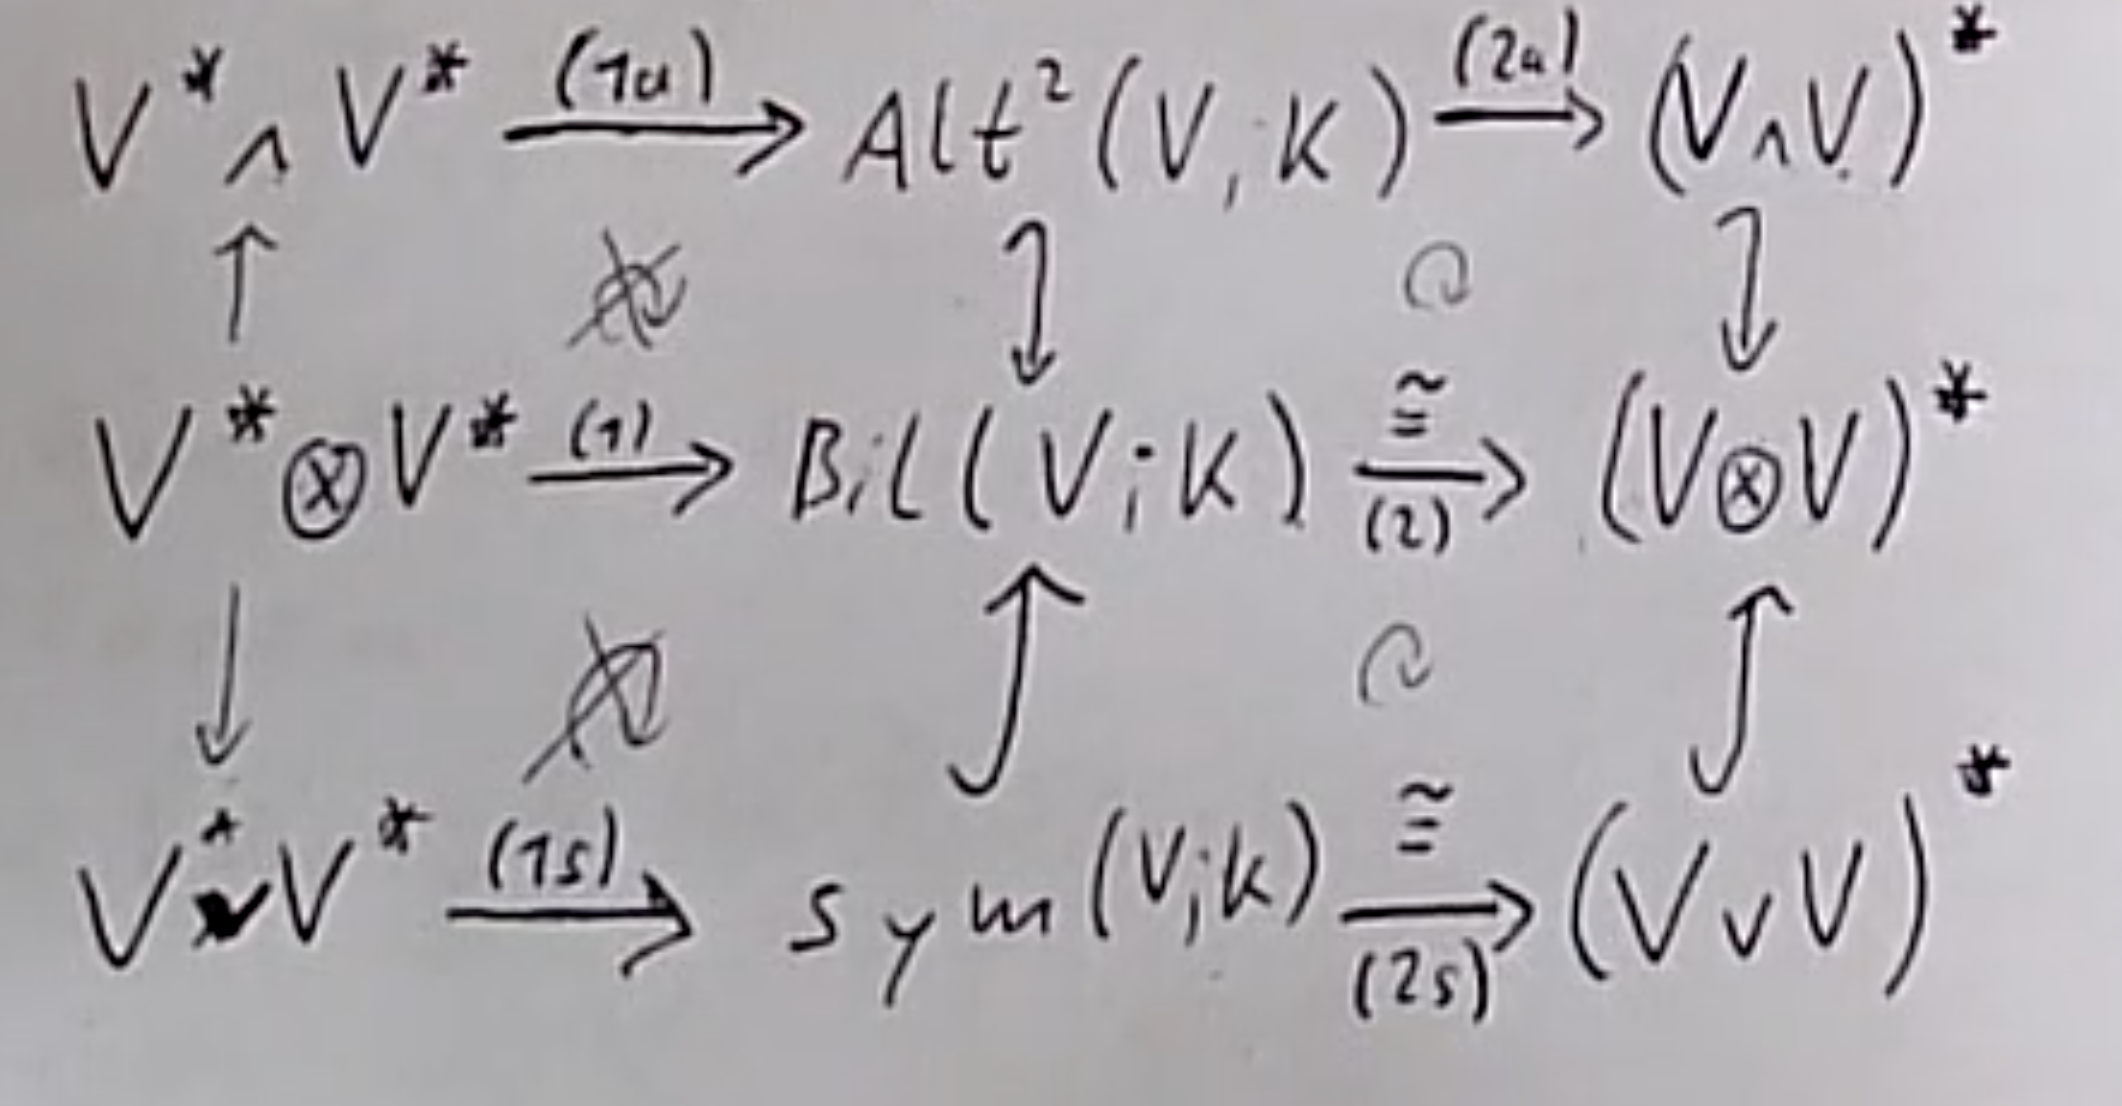
\includegraphics[scale=0.4]{Diagramm}

%Guter Editor: https://tikzcd.yichuanshen.de
\begin{equation*}
\begin{tikzcd}
V^* \wedge V^* \arrow[r, "{(1a), \cong^*}"]                     & \mathrm{Alt}^2(V;K) \arrow[r, "{(2a), \cong}"] & (V \wedge V)^*  \\
V^* \otimes V^* \arrow[u] \arrow[r, "{(1), \cong^*}"] \arrow[d] & \mathrm{Bil}(V;K) \arrow[r, "{(2), \cong}"]    & (V \otimes V)^* \\
V^* \vee V^* \arrow[r, "{(1s), \cong^{*,2}}"]                   & \mathrm{Sym}(V;K) \arrow[r, "{(2s), \cong}"]   & (V \vee V)^*   
\end{tikzcd},
\end{equation*}
wobei $^*$ Isomorphie unter Vorraussetzung der endlichen Dimension ist und $^2$  unter der Vorraussetzung $\mathrm{char}(K) \neq 2.$
\begin{enumerate}
\item[(2)] Die Abbildungen $(2a)$ und $(2a)$ und $(2)$ erhalten wir aus den universellen Eigenschaften.
\item[(1)] Folgt aus vorigem Theorem.
\item[(1a)]
Dieser Isomorphimus ist die lineare Abbildung zu der alternierenden Abbildung:
$$ 
\gamma: V^* \times V^* \rightarrow \mathrm{Alt}^2(V;K), \quad
\gamma(\varphi, \psi)(v, w):=\operatorname{det}\left(\begin{array}{cc}\varphi(v) & \varphi(w) \\ \psi(v) & \psi(w)\end{array}\right).
$$
\item[(1s)]
Dieser Isomorphismus ist die lineare Abbildung zu der symmetrischen Abbildung:
$$
\mu: V^* \times V^* \rightarrow \mathrm{Sym}^2 (V;K)
, \quad 
\mu(\varphi, \Psi)(v, w) := \operatorname{det}\left(\begin{array}{cc}\varphi(v) & - \varphi(w) \\ \psi(v) & \psi(w)\end{array}\right)
$$
\end{enumerate}
\end{example}

\comment{
\begin{theorem}
Ist $\mathrm{dim}V < \infty$, so ist $(1a)$ ein Isomorphismus und falls zus"atzlich $\mathrm{char}K = 2$, so ist $(1s)$ auch ein Isomorphismus.
\end{theorem}
}

\begin{definition}
Seien $V, V', W, W'$ Vektorr"aume und $F \in \mathrm{Hom}(V, V')$, $G \in \mathrm{Hom}(W, W')$. Dann definiert man das Tensorprodukt dieser Abbildungen folgendermassen als lineare Abbildung
$$
F \otimes G: V \otimes W \rightarrow V' \otimes W',
$$
so dass $(F \otimes G)(v \otimes w) = F(v) \otimes G(v)$ f"ur alle $v\in V, w \in W$.
\end{definition}
%Isomorphe Eigenschaft hinzufuegen? 

\begin{theorem}
F"ur endlichdimensionale Vektorr"aume $V, V', W, W'$ ist das Tensorprodukt von Abbildungen 
$$
\otimes: \mathrm{Hom}(V, V') \otimes  \mathrm{Hom}(W, W') \rightarrow \mathrm{Hom}(V \otimes W, V' \otimes W')
$$
ein Vektorraumisomorphismus.
\end{theorem}


\comment{
%Diesen Abschnitt muss man in einem anderen Abschnitt, zB bei den euklidischen und unitaeren Vektorrauemen, sinnvoll als subsection eingliedern
\section{Singul"arwertzerlegung und ihre Anwendungen}
\subsection{Die Singul"arwertzerlegung}

\begin{definition}
Man schreibt als Notation $\overline{V}^T = \tilde{V}^{\dagger}$.
\end{definition}

\begin{definition} \textbf{(Singul"arwertzerlegung)} Sei $K = \mathbb{R}$ oder $K = \mathbb{C}$ und $A \in M(m \times n, K)$. Dann gibt es orthogonale  / unit"are Matrizen $U \in O(m)$ / $U \in U(m)$, $V \in O(n)$ / $V \in U(n)$ und eine " diagonale Matrix  " $D\in M(m \times n, \mathbb{R})$ der Form 
$$
D=\left(\begin{array}{cccc}\sigma_{1} & 0 & \dots & 0 \\ 0 & \sigma_{2} & \dots & 0 \\ \vdots & & \ddots & \vdots\end{array}\right)
$$
mit nichtnegativen Diagonaleintr"agen $\sigma_j$, so dass
$$
A = U D V^\dagger.
$$
Diese Zerlegung heisst Singul"arwertzerlegung und die Diagonaleintr"age von $D$ $\sigma_1 \geq \sigma_2 \geq ... \geq \sigma_{\mathrm{min}(m,n)}$ heissen Singul"arwerte von $A$. Sie folgt aus dem Spektralsatz.

\end{definition}

\begin{remark}
Der Rang von $A$ entspricht dem Rang von $D$.
\end{remark}


\begin{corollary}
Zu $A \in M(m \times n, K)$ vom Rang $r$ gibt es gibt es orthogonale  / unit"are Matrizen $\tilde{U} \in M(m \times r, K)$, $\tilde{V} \in M(n \times r, K)$ mit orthonormalen Spalten und eine eine invertierbare Diagonalmatrix $\tilde{D} = \mathrm{diag}(\sigma_1, ..., \sigma_k) \in M(r \times r, \mathbb{R})$, so dass 
$$
A = \tilde{U} \tilde{D} \tilde{V}^\dagger.
$$
\end{corollary}


\begin{remark}
Um die Zerlegung aus obigem Korollar aus obigem Theorem zu erhalten, ordnet man die Singul"arwerte und definiert $\tilde{U}$ als die ersten $r$ Spalten von $U$ und $\tilde{V}$ als die ersten $r$ Spalten von $V$.

Umgekehrt erh"alt man $U$ aus $\tilde{U}$ bzw. $V$ aus $\tilde{V}$ indem man die durch die Spalten gegebene orthonormale Familie zu einer ONB erweitert und die entstehenden Vektoren als zus"atzliche Spalten schreibt. Bei $D$ f"ullt man die restlichen Zeilen mit $0$ auf.
\end{remark}



\begin{definition}
Die ersten $\mathrm{min}(m, n)$ Spalten von $U$ bzw. $V$ sind linke bzw. rechte Singul"arwerte von $A$. Man nennt Einheitsvektoren $u \in K^m$, $v \in K^n$ linke bzw. rechte Singul"arvektoren zum Singul"arwert $\sigma \in \mathbb{R}_{\geq 0}$, falls gilt
$$
Av = \sigma u \text{ oder } A^\dagger u = \sigma v
$$
\end{definition}

\begin{corollary}
Sei $F \in \mathrm{Hom}(V, W)$ mit $V, W$ endlich dimensional und unit"ar / euklidisch. Dann gibt es Orthonormalbasen $\mathcal{A}$ und $\mathcal{B}$, so dass 
$$
M^\mathcal{A}_\mathcal{B}(F) = D
$$
Diagonalform mit nichtnegativen Diagonaleintr"agen hat.
\end{corollary}

\begin{lemma}
Sei $A \in M (m \times n, K)$ eine beliebige Matrix vom Rang $r$. Dann sind die hermiteschen / symmetrischen Matrizen $\overline{A}^T A$, $A\overline{A}^T$ positiv semidefinit und haben Rang $r$. Es gilt
$$
\mathrm{Ker} \overline{A}^T A = \mathrm{Ker} A
$$
und
$$
\mathrm{Im} A \overline{A}^T = \mathrm{Im} A.
$$
\end{lemma}



\begin{remark}
Die Singul"arwerte von $A$ sind durch $A$ eindeutig bestimmt und sind die Wurzeln der gr"ossten $\mathrm{min}(m, n)$ Eigenwerte von $AA^\dagger$.. Die Matrizen $U$ und $V$ sind aber nicht ganz eindeutig bestimmt.
\end{remark}

%SVD Berechnung remark
\begin{remark} \bt{(Berechnung der Singul"arwertzerlegung)}
Sei $A \in M(m \times n, K)$.
\begin{enumerate}
\item Setze $B = A^\dagger A$ und bestimme die Eigenwerte $\lambda_1 \geq ... \geq \lambda)n \geq 0$ mit und orthogonalen Eigenvektoren $v_1, ..., v_n$ von $B$.
\item Setze $u_i = \frac{1}{\sqrt{\lambda_i}} A v_i$ f"ur $i = 1, ..., r$, wobei $\lambda_r$ der letzte positive Eigenwert ist.
\item Erg"anze $u_{r+1}, ..., u_m$ orthogonal zu $u_1, ..., u_r$.
\item Setze $U = (u_1, ..., u_m)$, $V = (v_1, ..., v_n)$, $D = \mathrm{diag}(\sqrt{\lambda_1}, ..., \sqrt{\lambda_k}, 0, ..., 0) \in M(m \times n, K)$.
\end{enumerate}
\end{remark}


%Analogon Satz Courant Fischer
\begin{corollary}
Sei $A \in M(m \times n, K)$ eine Matrix und die Singul"arwerte von $A$ gegeben durch
$$
\sigma_1 \geq ... \geq \sigma_p \geq 0.
$$
Dann folgt aus dem Satz von Courant-Fischer:
$$
\sigma_j = \min\limits_{U \subset K^n \atop \mathrm{dim}U = n-j+1} \left(   \max\limits_{u \in U \atop u \neq 0} \frac{\|Au\|}{\|u\|}\right) = \min\limits_{U \subset K^m \atop \mathrm{dim} U = m - j + 1} \left(   \max\limits_{ u \in U \atop u \neq 0 } \frac{ \|A^\dagger u\| }{ \|u\| } \right).
$$
\end{corollary}


\begin{definition}
Die Spektralnorm (2-Norm) einer Matrix $A \in M(m \times n, K($ ist der maximale Singul"arwert von $A$.
$$
\|A\|_{2}:=\sigma_{1}(A)=\max _{u \in K^n \atop u \neq 0} \frac{\|A u\|}{\|u\|}=\max _{u \in K^n \atop \|u\|=1}\|A u\|
$$
\end{definition}

\begin{remark}
Allgemeiner kann man f"ur $F \in \mathrm{Hom}(V, W)$, $V, W$ endlich dimensionale normierte Vektorr"aume, so eine Operatornorm definieren:
$$
\|F\|_{V, W} = \max\limits_{ v \in V \atop v \neq 0} \frac{\|F(v)\|_W}{\|v\|_V}.
$$
\end{remark}

%Es gab einen zusaetzlichen Abschnitt ueber die Anwendung der SVD in Regression und Pseudoinverse, der mir aber als irrelevant fuer die Klausur erschien und eher in den Bereichn Numerik faellt

%13052020

\subsection{Approximation von Matrizen durch Matrizen kleinen Ranges}
\begin{definition}
Sei $A = (a_{ij}) \in M( m \times n, K)$. Dann definieren wir die Frobeniusnorm von $A$ als
$$
\|A\|_F := \sqrt{\sum\limits_{i = 1}^m \sum\limits_{j = 1}^n |a_{ij}^2|} = \sqrt{\mathrm{tr}(A^\dagger A)}.
$$
Das ist die euklidische Norm von der Matrix aufgefasst als $m \cdot n$-Vektor, kommt also von folgendem Skalarprodukt auf $M(m \times n, K)$:
$
\scp{A}{B} = \mathrm{tr}(B^\dagger A).
$
\end{definition}



\begin{lemma}
Sei $A \in M( m \times n, K)$ und $U \in U(m)$, $V \in U(n)$. Dann:
$$
\| A \|_F = \|UAV\|_F.
$$
Insbesondere ist also f"ur $p = \min(m, n)$ dann
$
\|A\|_F =  \sqrt{\sigma_1^2 + ... + \sigma_p^2}.
$
\end{lemma}

\begin{theorem} \textbf{(Eckart-Young-Mirsky)} Sei $A = UDV^\dagger$ die Singul"arwerte von $A$ und seien die Singul"arwerte $\sigma_1 \geq  \sigma_2 \geq...$. Seien $u_1, ..., u_m \in K^m$ die Spalten von $U$ und $v_1, ..., v_n \in K^n$ die Spalten von $V$. Seien $U_k$ und $V_k$ die Matrizen bestehend aus den ersten $k$ Spalten von $U$ bzw. $V$. Sei $D_k$ die Matrix mit den ersten $k$ gr"ossten Singul"arwerten auf der Diagonalen. Sei 
$$
A_k = U_k D_k V_k^\dagger = \sum\limits_{j = 1}^k \sigma_j u_j v_j^\dagger.
$$
Dann gilt f"ur jede Matrix $B \in M( m \times n, K)$ vom Range $\leq k$, dass
$$
\|A - B\|_F \geq \|A - A_k \|_F = \sqrt{\sum\limits_{j = k+1}^r \sigma_j^2}.
$$
\end{theorem}

\begin{remark}
Es gilt f"ur jede Matrix $B \in M( m \times n, K)$ vom Rang $\leq k$, dass \\
$
\|A - B\|_2 \geq \|A - A_k \|_2 = \sigma_{k+1},
$
wobei $A_k$ wie oben ist.
\end{remark}

\begin{corollary}
Sei $A, B \in M(m \times n, K)$ und $i, j = 1, 2, ...$ beliebig. Dann gilt
$$
\sigma_{i+j-1} (A+B) \leq \sigma_i(A) + \sigma_j(B), 
$$
wobei $ \sigma_i(A)$ der $i$-te Singul"arwert von $A$ ist. Ist ein Index gr"osser als $\min(m, n),$ definiert man den entsprechenden Singul"arwert als $0$.
\end{corollary}

\begin{remark}
Die Singul"arwerte von $A - A_k$ sind $\sigma_{k+1}, \sigma_{k+2}, ... .$
\end{remark}

\subsection{Approximation durch orthogonale Matrizen}
\begin{theorem}
Sei $A \in M(n \times n, \mathbb{C})$ und $A = UDV^\dagger$ die Singul"arwertzerlegung. Dann minimiert $R_0 = UV^\dagger$ den Abstand 
$$
\|A - R\|_F
$$
unter allen unit"aren Matrizen $R \in U(n)$.
\end{theorem}
%B
%Zu Jordansche Normalform packen 
%Urspruengliche Theoreme kompakter machen mit zusammengefasster Version von Willwacher
}
%Siehe oben
\comment{
%15052020
\section{Verallgemeinerte Jordansche Normalform}
%Notationen von Willwacher notieren
\subsection{Relle Jordansche Normalform}
%aus LA I
\begin{theorem}
Sei $f \in \mathbb{R}[t]$ ein reelles Polynom vom Grad $n \geq 1$. Dann hat $f$ eine Zerlegung
$$
f = a(t - \lambda-1)...(t- \lambda_k)g_1...g_m,
$$
wobei $a \in \mathbb{R}$ und $\lambda_j \in \mathbb{R}$ die reellen Nullstellen sind und die $g_j \in \mathbb{R}[t]$ normierte quadratische Polynome ohne reelle Nullstellen sind. Insbesondere ist hier $n = k + 2m$, und falls $n$ ungerade ist muss $f$ mindestens eine reelle Nullstelle haben.
\end{theorem}

%Ausfuehrugen / Vorbereitung aus Skript uebernehmen?

\begin{theorem}
Sei $F$ ein Endomorphismus des $n$-dimensionalen $\mathbb{R}$-Vektorraums $V$. Seien $\lambda_1, ..., \lambda_k$, $g_1, ..., g_m, q_q, ..., q_m$ wie vorher. Sei
$$
V_j = \mathrm{Ker}(F- \lambda_j id_v)^{r_j}
$$
f"ur $j = 1, ..., k$ und 
$$
V_j' = \mathrm{Ker}(g_j(F))^{q_j}
$$
f"ur $j = 1, ..., m$.
Sei 
$$
d_{j r}= \operatorname{dim} \operatorname{Ker}\left(F-\lambda_{j} i d_{V}\right)^{r}
$$
$$
d_{j r}^{\prime}=\operatorname{dim} \operatorname{Ker}\left(g_{j}(F)^{r}\right)^{r}
$$
f"ur $r = 1, 2, ...$, und setze $d_{jr} = d_{jr}' = 0$ f"ur $r \leq 0$. Dann gilt:
\begin{enumerate}
\item Es gilt \(\operatorname{dim} V_{j}=r_{j}\) und \(\operatorname{dim} V_{j}^{\prime}=2 q_{j}\) und \(V\) zerf"allt in $F$ -invariante Untervektorräume:
$$
V=V_{1} \oplus \cdots \oplus V_{k} \oplus V_{1}^{\prime} \oplus \cdots \oplus V_{m}^{\prime}
$$
\item Es gibt eine Basis $\mathcal{B}$ von $V$ so dass:
%Matrix korrigieren
$$
M_\mathcal{B}(F)=
\left(\begin{array}{cccc}J_{1}\left(\lambda_{1}\right)^{\oplus s_{11}} & & & \\ 
& \ddots & \\ & J_{r_{k}}\left(\lambda_{k}\right)^{\oplus s_{k r_{k}}} & \\ 
& J_{1}\left(A_{1}\right)^{\oplus s_{11}^{\prime}} & J_{2}\left(A_{1}\right)^{\oplus s_{12}} & \\ 
& \ddots & J_{q_{1}}\left(A_{1}\right)^{\oplus s_{i q_{1}}} & J_{1}\left(A_{2}\right)^{\oplus s_{2 q_{1}}} \\ 
& & \ddots & J_{q_{m}}\left(A_{m}\right)^{\oplus s_{m, n}}
\end{array}\right)
$$
mit $A_j = \left(\begin{array}{cc}a_{j} & b_{j} \\ -b_{j} & a_{j}\end{array}\right)$, $\mu_j = a_j + i b_j$ wie vorher, und 
$$
s_{jr}=2 d_{j r}-d_{j(r+1)}-d_{j(r-1)}
$$
für $j=1, ..., k$ und alle $r$ und
$$
2 s_{j r}^{\prime}=2 d_{j r}^{\prime}-d_{j(r+1)}^{\prime}-d_{j(r-1)}^{\prime}
$$
für $j=1, ..., m$ und alle $r$.

\item Das Minimalpolynom ist 
$$
M_F(t) = (t - \lambda_1)^{l_1} ... (t - \lambda_k)^{l_k} g_1^{l'_1} ... g_m^{l'_m}
$$
mit $l_j$ bzw. $l_j'$ den gr"ossten Indizes mit $s_{jl_j}\neq 0$ bzw. $s_{jl_j'}' \neq 0$.

\end{enumerate}
\end{theorem}


\begin{corollary}
Zwei reelle Matrizen sind $"ahnlich$ "uber $\mathbb{R}$ ($A = S B S^{-1}$ mit $S \in GL(n, \mathbb{R})$) genau dann, wenn ihre charakteristischen Polynome und alle Zahlen $d_{jr}, d_{jr}'$ (wie im Theorem) "ubereinstimmen.
\end{corollary}

\begin{corollary}
Alle reellen Matrizen sind "uber $\mathbb{R}$ "ahnlich genau dann, wenn sie "ahnlich "uber $\mathbb{C}$ sind.
\end{corollary}
 
 %20052020
 
 \begin{corollary}
 Jede relle Matrix ist "ahnlich zu ihrer Transponierten. 
 \end{corollary}
 
 %Teile von Algebra Vorlesung nicht pruefungsrelevant
 \subsection{Jordansche Normalform f"ur allgemeine K"orper}
 
 \begin{definition}
 Sei $f = t^n + a_{n-1}t^{n-1} + ... + a_0 \in K[t]$ ein Polynom vom Grad $n$. Dann ist die Begleitmatrix von $f$ die Matrix 
 $$
 B_{f}:=\left(\begin{array}{ccccc}-a_{n-1} & 1 & 0 & \cdots & 0 \\ -a_{n-2} & 0 & 1 & \cdots & 0 \\ \vdots & \ddots & \ddots & \ddots & \vdots \\ -a_{1} & 0 & \cdots & \cdots & 1 \\ -a_{0} & 0 & \cdots & \cdots & 0\end{array}\right)
 $$
 \end{definition}
 
 \begin{theorem}
 Das charakteristische Polynom und das Minimalpolynom von $B_f$ sind bis auf ein Vorzeichen gleich $f$, also:
 $$
 (-1)^n P_{B_f} = M_{B_f} = f.
 $$
 \end{theorem}
 
 \subsubsection{Teilbarkeitstheorie von Polynomen}
 \paragraph{Zusammenfassung Aussagen "uber Polynomringe K[t] aus LA1}
 \begin{itemize}
 \item Sei $R$ ein kommutativer Ring und $f, g \in R, f, g \neq 0$. Dann heisst $f|g$, dass ein $h \in R$ existiert mit $g = fh$
 \item Ein Ideal $\mathcal{I} \subset R$ des kommutativen Ringes ist ein Unterring mit $\mathcal{I}R \subset \mathcal{I}$. Explizit: f"ur $f, g \in \mathcal{I}$ gilt $f-g \in \mathcal{I}$ und f"ur $f \in \mathcal{I}, g \in R$ gilt $fg \in \mathcal{I}$. 
 \\
 Sind $\mathcal{I}_1, \mathcal{I}_2$ Ideale, ist $\mathcal{I}_1 \cap \mathcal{I}_2$ und $\mathcal{I}_1 + \mathcal{I}_2$ (kleinstes Ideal das beide enth"alt) wieder Ideale
 \item F"ur jeden K"orper $K$ ist der Polynomring $K[T]$ ein Hauptidealring, d.h. zu jedem Ideal $\mathcal{I} \subset R$, $\mathcal{I} \neq \{0\}$ gibt es ein eindeutiges Polynom $M)\mathcal{I} \in \mathcal{I}$, so dass $\mathcal{I} = \{ M_\mathcal{I}f| f\in K[T]\}$. $M_\mathcal{I}$ ist das normierte Polynom kleinsten Grades in $\mathcal{I}$ und heisst Minimalpolynom von $\mathcal{I}$.
 \item F"ur jeden K"orper ist $K[t]$ ein faktorieller Ring, hat also keinen Nullteiler
 \end{itemize}
 
 
 \begin{definition}
 F"ur Polynome $f, g \in K[t], f, g \neq 0$ definieren wir den gr"ossten gemeinsamen Teiler (ggT) als das normierte Polynom vom gr"ossten Grad, das $f$ und $g$ teilt. Dies ist auch das Minimalpolynom vom Ideal von $f K[t] + g K[t]$, also $ggT(f, g) = M_{ K[t] + g K[t]}.$
 Also existieren $a, b \in K[t]$, so dass $ggT(f, g) = af + bg$.
 \\
 Allgemeiner ist $ggT(f_1, ..., f_n)$ das Polynom gr"ossten Grades, das alle $f_j$ teilt. Wiederum gibt es dann $a_1, ..., a_n \in K[t]$, so dass 
 $$
 ggT(f_1, ..., f_n) = a_1 f_1 + ... + a_n f_n
 $$
 
 Ebenso definiert man $kgV(f_1, ..., f_n)$ als das normierte Polynom kleinsten Grades, dass durch alle $f_j$ teilbar ist. 
 $$
 kgV(f_1, ..., f_n) = M_{f_1K[t] \cap ... \cap f_n K[t]}.$$
 \end{definition}
 
 \begin{lemma}
 F"ur ein Polynom $f \in K[t]$ positiven Grades sind "aquivalent:
\begin{itemize}
\item Aus $f = gh$ folgt, dass eis ein $0 \neq c \in K$ existiert, so dass $f = cg$ oder $f = ch$. (Also hat $f$ keine nichttrivialen Teiler, also nur die Teiler $c \in K$ und $cf$, ist also irreduzibel.)
\item Aus $f|gh$ f"ur $g, h \in K[t], g, h \neq 0$ folgt, dass $f|g$ oder $f|h$. (Man sagt dann auch, dass $f$ ein Primelement ist).
\end{itemize}
 \end{lemma}
 
 
 
 \begin{theorem} (Primfaktorzerlegung f"ur Polynome)
 Sei $0 \neq f \in K[t]$ ein Polynom. Dann gibt es irreduzible normierte Polynome $p_1, ..., p_n \in K[t]$ positiven Grades und $c \in K$ $c\neq 0$, so dass
 $$
 f = cp_1 ... p_n.
 $$
 Diese Faktorisierung ist eindeutig bis auf die Anordnung der $p_j$.
 Man sagt auch $K[t]$ ist ein faktorieller Ring.
 \end{theorem}
 
 
 
 \begin{definition}
 Ein Ideal $\mathcal{I} \subset R$ des kommutativen Ringes $R$ heisst \bt{maximal}, falls $\mathcal{I} \neq R$ und es kein Ideal $\mathcal{J}$ gibt, so dass 
 $$
\mathcal{I} \varsubsetneqq \mathcal{J} \varsubsetneqq R.
 $$
 $\mathcal{I}$ heisst Prim, falls $\mathcal{I} \neq R$ und f"ur alle $f, g \in R$ gilt $fg \in \mathcal{I} \implies
  f \in \mathcal{I} \vee g \in \mathcal{I}$.
 \end{definition}
 
 \begin{remark}
 Im Fall $R = K[t]$ folgt direkt aus der Definition, dass $\mathcal{I}$ ein Primideal ist genau dann, wenn $M_\mathcal{I}$ prim. Ebenso ist $\mathcal{I}$ maximal, genau dann wenn $M_\mathcal{I}$ irreduzibel ist.
 \end{remark}
 
 \begin{lemma}
 Sei $\mathcal{I} \varsubsetneqq R$ ein Ideal im kommutativen Ring $R$ mit Eins. Dann gilt \begin{itemize}
 \item $\mathcal{I}$ ist maximal genau dann, wenn $R / \mathcal{I}$ mit der von $R$ geerbten Addition und Multiplikation ein K"orper ist.
 \item $\mathcal{I}$ ist prim genau dann, wenn $R/ \mathcal{I}$ nullteilerfrei ist.
 \end{itemize}
 Hierbei ist $R / \mathcal{I} = R / \sim$ mit $f \sim g \Leftrightarrow f - g \in \mathcal{I}$ definiert. Man schreibt $f + \mathcal{I} \in R / \mathcal{I}$ f"ur die "Auivalenzklasse von $f \in R$. 
 \end{lemma}
 
 
 %nicht pruefungsrelevantes Kapitel
 \subsection{Jordan'sche Normalform}
 
 \begin{definition}
 Wir definieren die Matrix
 $$
 \tilde{E}_n =
\left(\begin{array}{cccc}0 & 0 & \cdots & 0 \\ \vdots & \ddots & \ddots & \vdots \\ 0 & 0 & \cdots & 0 \\ 1 & 0 & \cdots & 0\end{array}\right) \in M(n \times n, K)
 $$
 und 
 $$
 \tilde{J_r}(A)
=\left(\begin{array}{ccccc}A & \tilde{E}_{n} & & & \\ & A & \tilde{E}_{n} & & \\ & & \ddots & \ddots & \\ & & & \ddots & \tilde{E}_{n} \\ & & & & A\end{array}\right) \in M(n r \times n r, K).
 $$
 \end{definition}
 
 
 \begin{theorem}
 Sei $V$ ein endlich dimensionaler $k$-Vektorraum und $F \in End(V)$. Sei
 $$
 P_F = \pm p_1^{r_1} .... p_k^{r_k}
 $$
 die Faktorisierung in irreduzible normierte Polynome $p_1, ..., p_k$, die paarweise verschieden sind. Dann gibt es eine Basis $\mathcal{B}$ von $V$, si dass $M_\mathcal{B}(F)$ blockdiagonal ist mit Diagonalbl"ocken der Form $\tilde{J_r}(B_{p_f})$ mit $j = 1, ..., k$ und $r = 1, ..., r_j$.
 \\ Sei dabei $s_{jr}$ die Anzahl Jordanbl"ocke der Gr"osse $\tilde{J_r}(B_{p_j})$. 
 Dann gilt f"ur alle $J$
 $$
 \sum\limits_{r = 1}^{r_j} s_{jr} = r_j \mathrm{deg} p_j
 $$
 und 
 $$
 s_{jr} = \frac{1}{\mathrm{deg}  p_j}(2 \mathrm{dim} \mathrm{Ker} (p_j(F)^r) -\mathrm{dim} \mathrm{Ker}(p_j(F)^{r+1}) - \mathrm{dim} \mathrm{Ker}(p_j(F)^{r-1}).
 $$
 Insbesondere ist die Jordan'sche Normalform bis auf eine Permutation der Diagonalbl"ocke eindeutig.
  
 \end{theorem}
 
 %27052020
 \begin{theorem}
 Sei $V$ ein endlich dimensionaler $K$-Vektorraum und $F \in \mathrm{End}(V)$ mit $P_f = \pm p_1^{r_1} ... p_r^{r_k}$ als irreduzible Faktorisierung. Sei 
 $$
 V_k = \mathrm{Ker}(p_j(F)^{r_j}).
 $$
 Dann sind alle $V_k$ $F$-invariant und
 $$
 V = V_1 \oplus ... \oplus V_k.
 $$
 Das charakterische Polynom der Einschr"ankung $F|V_j$ ist
 $$
 P_{F|V_j} = \pm p_j^{r_j}.
 $$
 Insbesondere als $\mathrm{dim}_K(V_j) = r_j \mathrm{deg}(p_j)$.
 \end{theorem}
 %E
 
 }
 
 
\section{N\uee tzliche Formeln und Hinweise}
\paragraph{Beweise Tricks}
\begin{enumerate}
\item Um einen Vektor in zwei verschiedenen Untervektorr"aumen zu suchen, zeige mit der Dimensionsformel, dass sie sich schneiden m"ussen. zB eingesetzt bei Eckart-Young-Mirsky Theorem, Beweis vom Satz von Courant-Fischer
\item Induktionsbeweise Invararianz von Untervekorr"aumen um die Induktionsvorraussetzung anzuwenden
\item Setze bei Optimierungsaufgaben unter der Frobeniusnorm die Singul"arwertzerlegung ein, da die Frobeniusnorm invariant unter orthogonalen Matrizen ist.
\item Man kann einem algebraisch abgeschlossenen K"orper oBdA annehmen, dass eine Matrix in (reeller) JNF ist
\item Um zu zeigen, dass eine lineare Abbildung zwischen zwei endlich dimensionalen Vektorr"aumen bijektiv ist, zeige, dass sie Basen auf Basen abbildet.
\item Um zu zeigen, dass eine Familie linear unabh"angig ist (zum Beispiel beim Beweis des symmetrischen Produkts), konstruiere einen Isomorphismus der die Familie auf eine Basis (zB des $K^n$) abbildet.
\end{enumerate}
\end{document}
